\documentclass[11pt]{article}

% Use wide margins, but not quite so wide as fullpage.sty
\marginparwidth 0.5in 
\oddsidemargin 0.25in 
\evensidemargin 0.25in 
\marginparsep 0.25in
\topmargin 0.25in 
\textwidth 6in \textheight 8 in

\usepackage{amsmath}
\usepackage{multirow}
\usepackage{tabularx}
\usepackage{longtable}
\usepackage{booktabs}
\usepackage[normalem]{ulem}
\useunder{\uline}{\ul}{}
\usepackage{graphicx}
\usepackage{epstopdf}
\usepackage{comment}
\usepackage[colorinlistoftodos]{todonotes}
\usepackage{float}
\usepackage{hyperref}
\usepackage{siunitx}
\usepackage{color}
\usepackage{enumitem}
\usepackage[utf8x]{inputenc}
\usepackage[italian]{babel}
\usepackage{amsmath}



\begin{document}
% this is an alternate method of creating a title
%\hfill\vbox{\hbox{Gius, Mark}
%       \hbox{Cpe 456, Section 01}  
%       \hbox{Lab 1}    
%       \hbox{\today}}\par
%
%\bigskip
%\centerline{\Large\bf Lab 1: Security Audit}\par
%\bigskip



\author{Gruppo 3: Danilo Bondì, Irene Cortinovis, Alfredo Guarnieri}
\title{Esperimentazioni di Fisica II}
\maketitle

\tableofcontents\newpage



%%%%%%%%%%%%%%%%%%%%%%%%%%%%%%%%%%%%%%%%%%%%%%%%%%%%    
%%% C1

\section{Circuiti 1}

\subsection{Parte 1 }

\subsubsection{Resistenze interne strumenti}
%    
    Chiamiamo $R_i$ la resistenza da misurare e $R_V$ la resistenza interna del voltmetro e $R_A$ la resistenza interna dell'amperometro.\\    
%  
    Le resistenze che abbiamo utilizzato sono le seguenti (errore letto da ultima cifra dello strumento di misura):
    %   Tabella dati resistenze
    \begin{table}[H]
        \centering
        \begin{tabular}{|l r|}
            \hline
            $R_1$ & $ 10.1 \pm 0.1\Omega$      \\
            $R_2$ & $ 677 \pm 1\Omega$         \\
            $R_3$ & $ 15970 \pm 10\Omega$      \\
            $R_4$ & $ 981000 \pm 1000\Omega$   \\ 
            $R_5$ & $ 149000 \pm 100\Omega$    \\ 
            \hline
        \end{tabular}
        %\caption{Caption}
        %\label{tab:my_label}
    \end{table}
    
    Schema dei due circuiti:
     % Schema circuiti
    \begin{figure}[H]
    \centering
    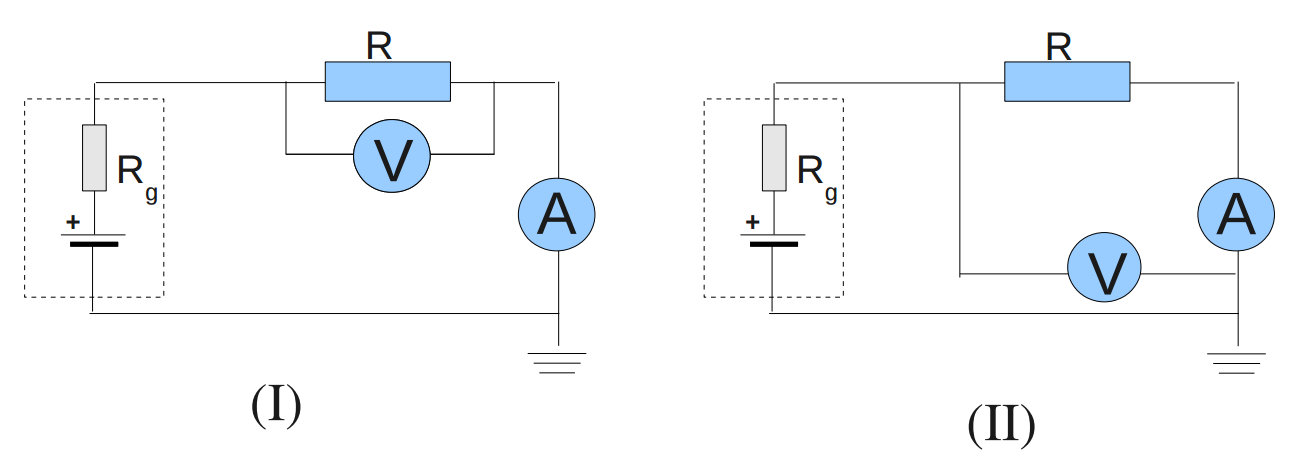
\includegraphics[scale=.25]{Grafici/C1_P1.png}
    \end{figure} 
    
    
    Formule utilizzate:
    $$ \Delta V = R_{eq} I \Rightarrow R_{eq}=\frac{\Delta V}{I}$$

    %spiegazione Rv
    Circuito 1: misura di $R_V$
    $$ \frac{1}{R_{eq}} = \frac{1}{R} + \frac{1}{R_V} \Rightarrow R_V = \frac{RR_{eq}}{R-R_{eq}} = \frac{R \Delta V}{IR - \Delta V} $$
    
    
    %spiegazione Ra
    Circuito 2: misura di $R_A$
    $$ R_{eq} = R + R_A \Rightarrow R_A = R_{eq} - R = \frac{\Delta V}{I} - R$$
    
    
    %   resistenza bassa
    %Abbiamo riscontrato che se $R$ è troppo bassa rispetto a $R_V$, le misure effettuate risultano alterate. Abbiamo attribuito questo effetto alla eccessiva differenza tra le due resistenze, che fa sì che la corrente passante attraverso $R_V$ non sia sufficiente per una misura corretta.  
   % Riportiamo in seguito i dati relativi a ciò.
%
    %   tabella schifo
    %\begin{table}[H]
\caption{Misure di $R_V$ usando resistenze basse}
\begin{tabular}{|c|c|c|c|c|}
\hline
Tensione V (V) & Corrente I (A) & Resistenza R ($\Omega$) & \textbf{Rv ($\Omega$)} & $fem$ (V) \\
\hline
0.561 & 5.75E-02 & 10.1 & 2.87E+02 & 0.90 \\ 
0.937 & 9.57E-02 & 10.1 & 3.20E+02 & 1.50 \\ 
1.657 & 1.69E-01 & 10.1 & 3.35E+02 & 2.00 \\ 
0.997 & 1.48E-03 & 677 & 4.29E+05 & 1.00 \\ 
2.982 & 4.41E-03 & 677 & 4.10E+05 & 3.00 \\
5.45 & 8.08E-03 & 677 & 2.20E+05 & 5.50 \\ \hline
\end{tabular}
\label{}
\end{table}
% 
%
    Dati sperimentali:
    %Tabella dati Rv%
    \begin{table}[H]
    \centering
    \caption{Misure di Resistenza Voltmetro}
    \begin{tabular}{|c|c|c|c|}
    \hline
        Tensione V(V) & Corrente I(A) & Resistenza R (k$\Omega$) & Resistenza $R_V$ ($\Omega$) \\
        $\pm 0.01\%$ & $\pm 3.92 \%$ & $\pm 0.27 \%$ & $\pm 4.47 \%$\\
        \hline
        5.504   & $3.45 \cdot10^{-1}$  & 15.97  & $1.56 \cdot10^4$ \\
        4.012   & $2.52 \cdot10^{-1}$  & 15.97  & $5.15 \cdot10^3$ \\
        6.507   & $4.08 \cdot10^{-1}$  & 15.97  & $1.19 \cdot10^4$ \\
        13.04   & $1.50 \cdot10^{-2}$  & 981.0  & $7.64 \cdot10^3$ \\
        7.510   & $8.00 \cdot10^{-3}$  & 981.0  & $2.18 \cdot10^4$ \\
        10.02   & $1.10 \cdot10^{-2}$  & 981.0  & $1.27 \cdot10^4$ \\
        5.012   & $3.40 \cdot10^{-2}$  & 149.0  & $1.38 \cdot10^4$ \\
        8.010   & $5.50 \cdot10^{-2}$  & 149.0  & $6.45 \cdot10^3$ \\
        11.02   & $7.50 \cdot10^{-2}$  & 149.0  & $1.06 \cdot10^4$ \\
        \hline
    \end{tabular}
    \label{}
\end{table} 
    %Tabella dati Ra
    \begin{table}[H]
    \centering
    \caption{Misure di Resistenza Amperometro}
    \begin{tabular}{|c|c|c|c|}
    \hline
        Tensione V(V) & Corrente I(A) & Resistenza R ($\Omega$) & Resistenza $R_A$ ($\Omega$) \\
        $\pm 0.03\%$ & $\pm 0.09 \%$ & $\pm 0.04 \%$ & $\pm 0.20 \%$\\
        \hline
            4.001 & 1.455 $\cdot 10^{-2}$ & 267.6 & 7.38 \\ 
            7.010 & 2.580 $\cdot 10^{-2}$ & 267.6 & 4.11 \\ 
            1.506 & 5.509 $\cdot 10^{-3}$ & 267.6 & 5.77 \\ 
            2.506 & 9.170 $\cdot 10^{-3}$ & 267.6 & 5.68 \\ 
            8.510 & 3.140 $\cdot 10^{-2}$ & 267.6 & 3.42 \\ \hline
    \end{tabular}
    \label{}
\end{table}

    
    
    Per $R_V$ e $R_A$, abbiamo stimato l'errore relativo percentuale dalla somma degli errori relativi di $V$ $R$ e $I$, trovando:
        $$ R_V = 1.17\cdot10^4 \; k\Omega \pm 4.47\%$$
        $$ R_A = 5.27 \Omega \pm 0.02 \% $$
% 
%
%
%
%
\subsubsection{Verifica legge di Ohm}
%
% 
%   
\textbf{Resistore 1}\\
%
    % Dati R1
    \begin{table}[H]
    \centering
    \begin{tabular}{|c|c||c|c|}
    \hline
        Tensione V 	&	Corrente I & Tensione V   &   Corrente I 	\\
        V	&	mA      & V &   mA	\\
        $\pm 0.001 (0.04\%)$	&	$\pm 0.01 $ & $\pm 0.001 (0.04\%)$   &   $\pm 0.01 $	\\ \hline
        0.503	&	0.74	&  5.459   &   8.09    \\
        0.996	&	1.47	&  5.949   &   8.81    \\
        1.497	&	2.21	&  6.446   &   9.56    \\
        1.992	&	2.95	&  6.950   &   10.30   \\
        2.488	&	3.68	&  7.440   &   11.03   \\
        2.982	&	4.41	&  7.940   &   11.78   \\
        3.473	&	5.14	&  8.430   &   12.52   \\
        3.972	&	5.88	&  8.930   &   13.27   \\
        4.471	&	6.62	&  9.430   &   14.00   \\
        4.964	&	7.35	&  9.920   &   14.75   \\ \hline
    \end{tabular}
    \caption{Dati per R1}
    \label{tab:R1_ohm}
\end{table}
%
    % Grafico R1
    \begin{figure}[H]
    \centering
    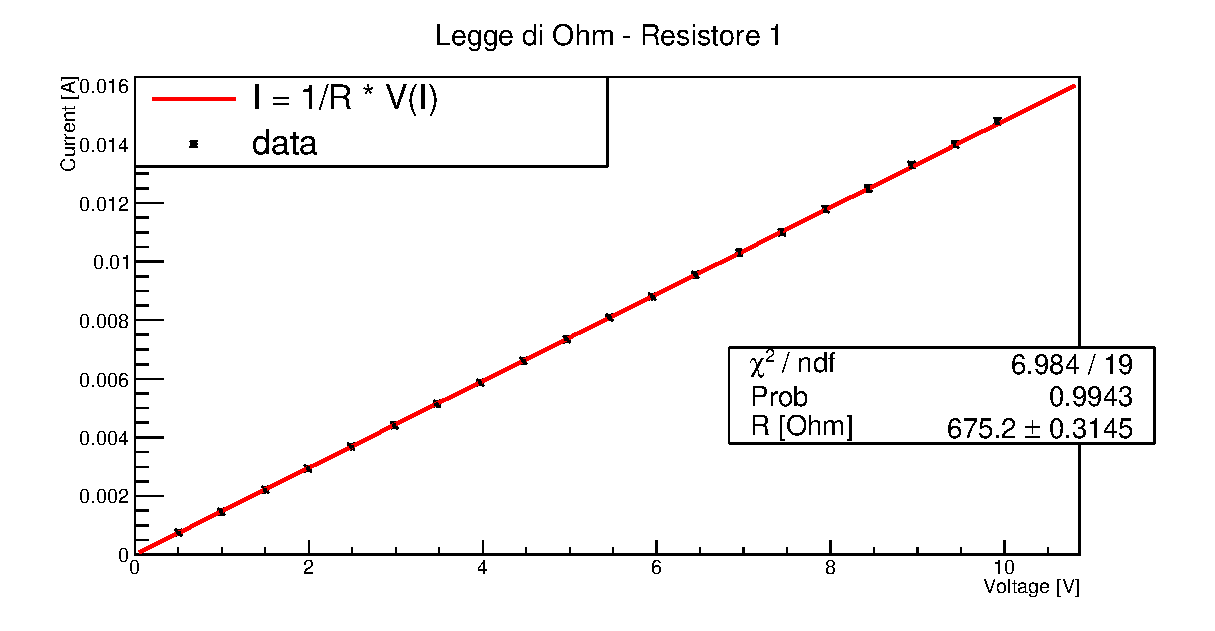
\includegraphics[scale=.8]{Grafici/C1_P1_ohmR1.eps}
    %\caption{Verifica legge di Ohm per resistore R1}
    \label{fig:C1_P1_OhmR1}
    \end{figure} 
%
    %   Resistore R1
    \begin{center}
   % \centering
    Valore misurato: $R_1 = 677 \pm 1  \Omega$  \\
    Valore ottenuto dal Fit: $R_1 = 675.2 \pm 0.3 \Omega$ \\
    \end{center}
%
    Il risultato è accurato anche se l'errore associato è probabilmente troppo basso.\\\\
%
% 
%
%
%
\textbf{Resistore 2}\\
%
    % Dati R2
    \begin{table}[H]
    \centering
    \begin{tabular}{|c|c||c|c|}
    \hline
        Tensione V 	&	Corrente I & Tensione V   &   Corrente I 	\\
        V	&	mA      & V &   mA	\\
        $\pm 0.001 (0.04\%)$	&	$\pm 0.01 $ & $\pm 0.001 (0.04\%)$   &   $\pm 0.01 $	\\ \hline
        0.249   &   0.94    &   2.699   &   10.15   \\
        0.493   &   1.89    &   2.940   &   11.05   \\
        0.744   &   2.80    &   3.184   &   11.98   \\
        0.983   &   3.96    &   3.427   &   12.89   \\
        1.233   &   4.63    &   3.674   &   13.83   \\
        1.477   &   5.55    &   3.914   &   14.73   \\
        1.722   &   6.47    &   4.163   &   15.68   \\
        1.959   &   7.36    &   4.403   &   16.59   \\
        2.212   &   8.31    &   4.652   &   17.52   \\
        2.448   &   9.21    &   4.892   &   18.44   \\ \hline
    \end{tabular}
    \caption{Dati per R2}
    \label{tab:R2_ohm}
\end{table}




       
        
        
%
    %   Grafico R2
    \begin{figure}[H]
    \centering
    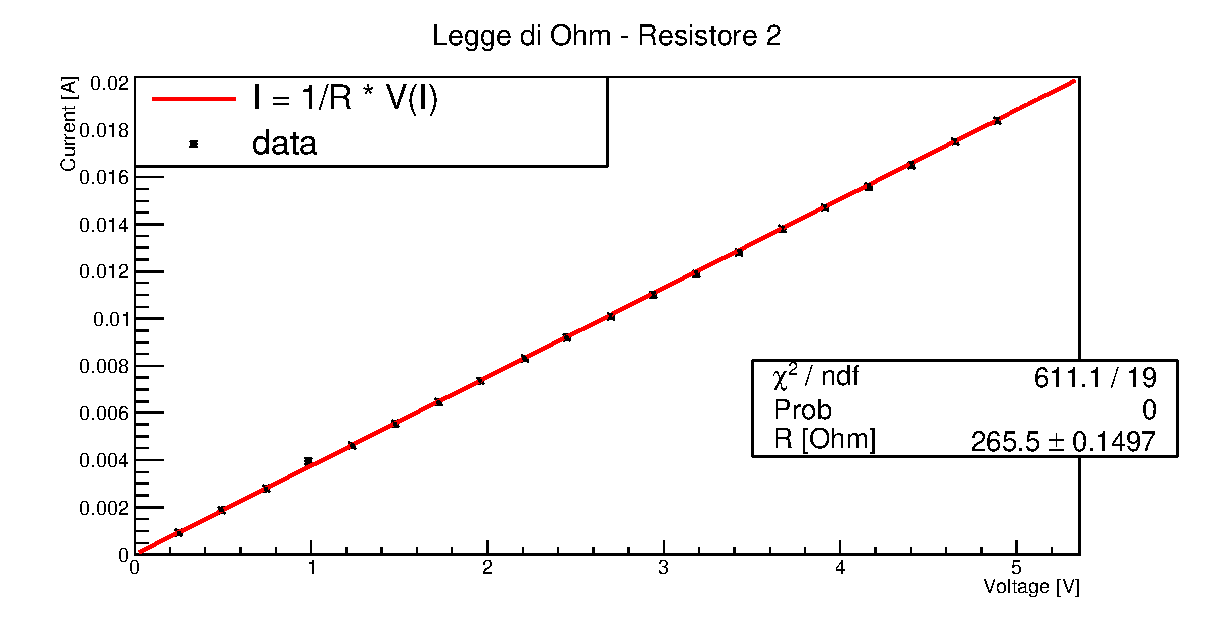
\includegraphics[scale=.8]{Grafici/C1_P1_ohmR2.eps}
    %\caption{Verifica legge di Ohm per resistore R2}
    \label{fig:C1_P1_OhmR2}
    \end{figure}
%
    %   Resistore R2
    \begin{center}
    %\centering
    Valore misurato: $R_2 = 266 \pm 1  \Omega$  \\
    Valore ottenuto dal fit: $ R_2 = 265.5 \pm 0.1 \Omega$ \\
    \end{center}
%
    In questo caso il chi quadro ridotto è molto alto. I dati sono molto scatterati rispetto alla linea, rispetto al loro errore. Siccome il risultato finale è accurato, il problema è probabilmente dovuto ad una sottovalutazione dell'errore associato alle misure.
%
\subsubsection{Resistenze composite}
    Errori considerati come ultima cifra decimale dello strumento di misura.\\
%
    Dati:\\
       $ R_1 = 148 \pm 1 k\Omega $\\ 
       $ R_2 = 149 \pm 1 k\Omega $\\ 
       $ R_3 = 100 \pm 1 k\Omega $\\ 
%     
%
    %Req serie
    \begin{table}[H]
\caption{Misure sperimentali con resistenze in serie}
\begin{tabular}{|c|c|c|c|c|}
\hline
    Combinazione & Tensione V (k$\Omega$) & Corrente I (mA) & Req (k$\Omega$) & Req teorica (k$\Omega$) \\ \hline
     & $\pm$ 0.001 &  $\pm$ 0.001 & $\pm$ 1 & \\ 
     \hline
    R1+R2   & 5.003 & 0.017 & 294 & 297 \\ 
            & 7.500 & 0.026 & 288 & 297 \\
            & 10.02 & 0.035 & 286 & 297 \\
    R1+R3   & 5.009 & 0.021 & 239 & 248 \\
            & 7.500 & 0.031 & 242 & 248 \\
            & 10.01 & 0.041 & 243 & 248 \\
    \hline
\end{tabular}
\label{}
\end{table}
%  
    %Req parallelo
    \begin{table}[H]
\caption{Misure sperimentali con resistenze in Parallelo}
\begin{tabular}{|c|c|c|c|c|}
\hline
    Combinazione & Tensione V (k$\Omega$) & Corrente I (mA) & Req (k$\Omega$) & Req teorica (k$\Omega$) \\ \hline
     & $\pm$ 0.001 &  $\pm$ 0.001 & $\pm$ 0.1 & \\ 
    \hline
    R1+R2   & 5.007 & 0.068 & 73.6 & 74.2 \\
            & 7.500 & 0.102 & 73.5 & 74.2 \\ 
            & 10.01 & 0.136 & 73.6 & 74.2 \\  \hline
    R1+R3   & 5.008 & 0.084 & 59.6 & 59.7 \\ 
            & 7.510 & 0.126 & 59.6 & 59.7 \\ 
            & 10.00 & 0.168 & 59.5 & 59.7 \\ \hline
\end{tabular}
\label{}
\end{table}
    
    Riassunto risultati:
    %risultati resistenza equivalente
    \begin{table}[H]
    \centering
    \caption{Risultati di Resistenza equivalente ottenuti}
    \begin{tabular}{|c|c|c|c|}
        \hline
        SERIE & Teorica (k$\Omega$) & Misurata (k$\Omega$) & Discrepanza \% \\ \hline
        R1+R2 & 297 & 290 $\pm$ 1 & 2\% \\ 
        R1+R3 & 248 & 241 $\pm$ 1 & 3\% \\ 
        \hline
        PARALLELO & Teorica (k$\Omega$) & M (k$\Omega$) & Discrepanza \% \\ \hline
        R1+R2 & 74 & 74 $\pm$ 1 & 1\% \\ 
        R1+R3 & 60 & 60 $\pm$ 1 & 1\% \\ \hline
    \end{tabular}
    \label{}
\end{table}
 

\newpage

\subsection{Parte 2 }

\subsubsection{Partitore resistivo}
%
    Schema del ciruito:
    %
    \begin{figure}[H]
    \centering
    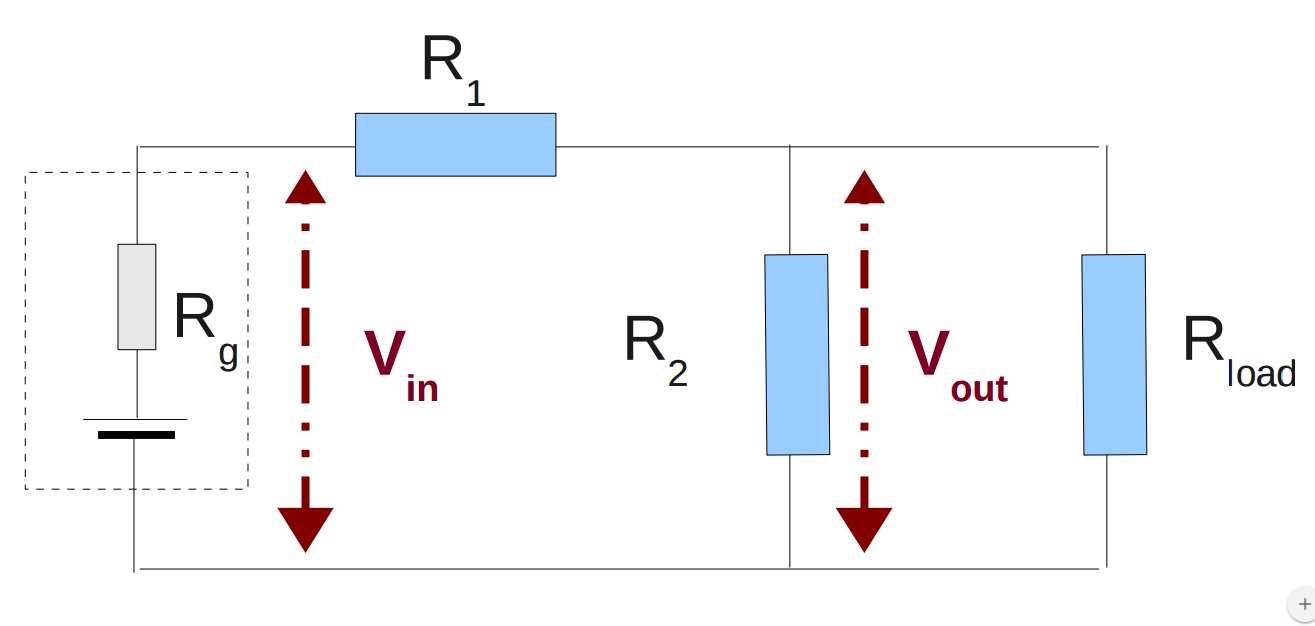
\includegraphics[scale=.25]{Grafici/C1_P2.png}
    \end{figure} 

    Affinchè $V_{out}$ sia circa metà di $V_{in}$ senza $R_L$, si ha che $R_1$ e $R_2$ devono essere circa uguali, in modo che la caduta di potenziale sia distribuita sui due resistori in modo uguale.\\
    Lasciando $R_1$ e $R_2$ uguali, abbiamo verificato due casi: resistenze basse e alte.\\
    Affinchè la caduta di potenziale su $R_L$ sia circa indipendente dal suo valore, occorre che $R_2$ sia molto minore di $R_L$ affinchè abbia peso maggiore nella resistenza equivalente, come dimostrato nei seguenti calcoli:
    $$ \Delta V = V_{R_1} + V_{R_L} = I R_1 + I \frac{R_2 R_L}{R_2 + R_L} = I R_1 + \frac{I R_2}{1 + \frac{R_2}{R_L}}  $$
    Se $ R_2$ molto minore di $R_L$, il denominatore tende a 1 e dunque $V_{R_L}$ non dipende da $R_L$.\\\\
    %
    \textbf{Dati sperimentali}\\\\
    %
    \textbf{Resistenze basse}\\
    %
    $R_L$ (kOhm) =	0.266	$\pm$ 0.001\\
    $R_2$ kOhm) =	0.268   $\pm$ 0.001\\
    %
    %
    %
    \begin{table}[H]
\centering
\caption{Resistenze basse}
\begin{tabular}{|c|c|c|}
\hline
$R_L$	&	$V_{in}$ 	&	$V_{out}$	\\
$[kOhm]$	&	$[V]$	&	$[V]$	\\
$\pm 1 kOhm$ 	&	$\pm 0.01 V$	&	$\pm 0.001 V$	\\ \hline
100	&	1.50	&	0.754	\\
100	&	3.00	&	1.503	\\
100	&	5.00	&	2.501	\\ \hline
149	&	1.50	&	0.757	\\
149	&	3.00	&	1.504	\\
149	&	5.00	&	2.500	\\ \hline
981	&	1.50	&	0.756	\\
981	&	3.00	&	1.505	\\
981	&	5.00	&	2.504	\\ \hline
\end{tabular}
\label{}
\end{table}
    %
    %
    Il seguente grafico mostra tutti i dati sulla stessa canvas. 
    % grafico
    \begin{figure}[H]
    \centering
    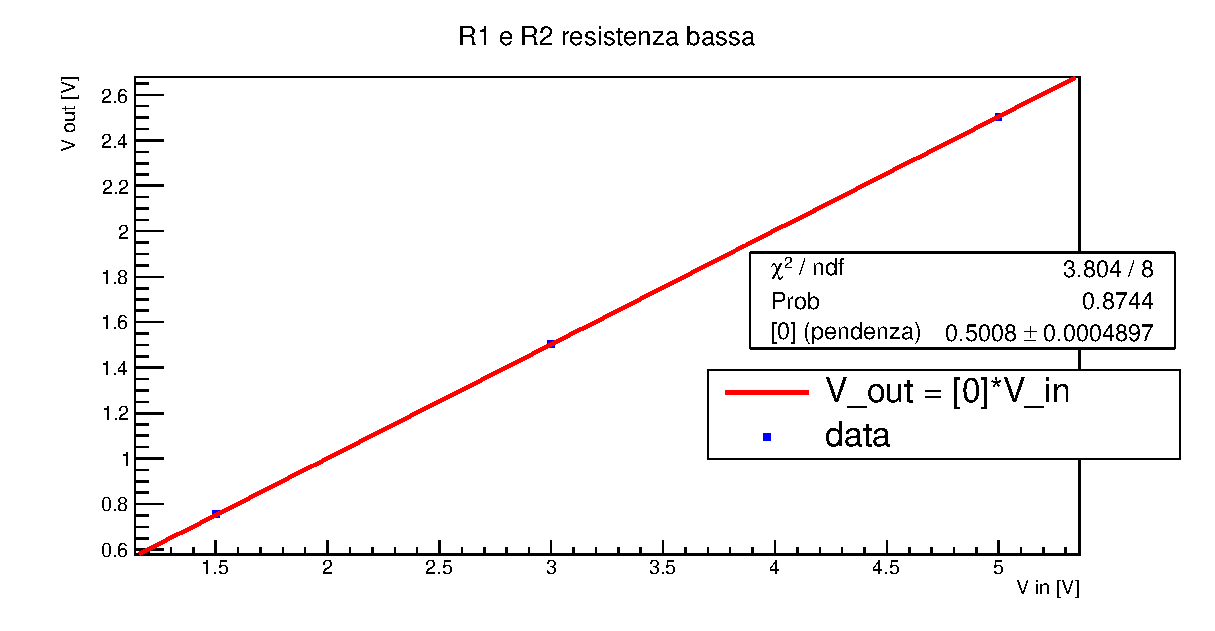
\includegraphics[scale=.7]{Grafici/C1_P2_partResLow.eps}
    \end{figure}
    %
    Si osserva che:
    \begin{itemize}
        \item  I valori sono 9 come riportato nella tabella, ma sono a tre a tre molto simili, quindi non si riescono a distinguere. Da questo segue che la caduta di tensione in $R_L$ non dipende da $R_L$. Infatti a parità di $V_{in}$, cambiando $R_L$ il $V_{out}$ non cambia.
        \item $V_{out} = 0.5 \cdot V_{in}$, con un chi quadro ridotto di 3.8/8.
    \end{itemize}
%
    \textbf{Resistenze alte}\\\\		
    $R_1$ (kOhm) =	978 $\pm$ 1\\
    $R_2$ (kOhm) =	981 $\pm$ 1\\
    %
    %
    \begin{table}[H]
\centering
\caption{Resistenze alte}
\begin{tabular}{|c|c|c|}
\hline
$R_L$	&	$V_{in}$ 	&	$V_{out}$	\\
$[kOhm]$	&	$[V]$	&	$[V]$	\\
$\pm 1 kOhm$ 	&	$\pm 0.01 V$	&	$\pm 0.001 V$	\\ \hline
0.677	&	5.24	&	0.004	\\
0.677	&	10.00	&	0.007	\\
0.677	&	14.00	&	0.010	\\ \hline
15.97	&	3.00	&	0.047	\\
15.97	&	5.00	&	0.079	\\
15.97	&	7.00	&	0.110	\\ \hline
100.1	&	3.00	&	0.253	\\
100.1	&	5.00	&	0.421	\\
100.1	&	7.00	&	0.589	\\ \hline
\end{tabular}
\label{}
\end{table}
    %
    I seguenti tre grafici mostrano i dati, suddivisi per $R_L$ utilizzata.
    %
    % grafico
    \begin{figure}[H]
    \centering
    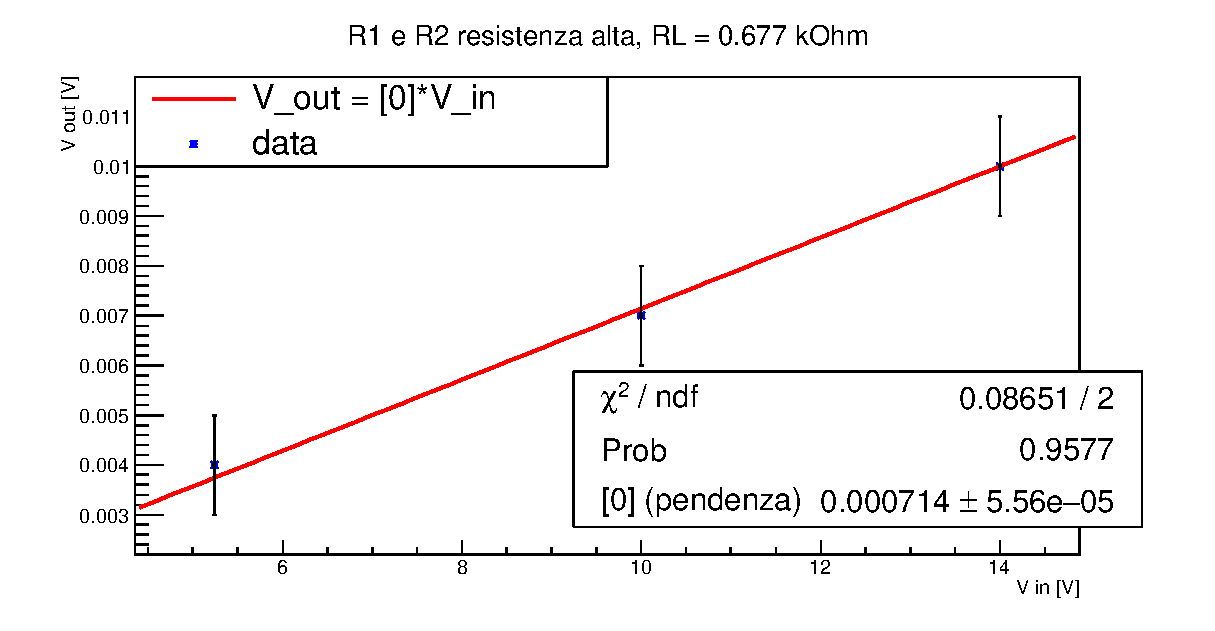
\includegraphics[scale=.7]{Grafici/C1_P2_partResHigh1.eps}
    \end{figure}
    
    \begin{figure}[H]
    \centering
    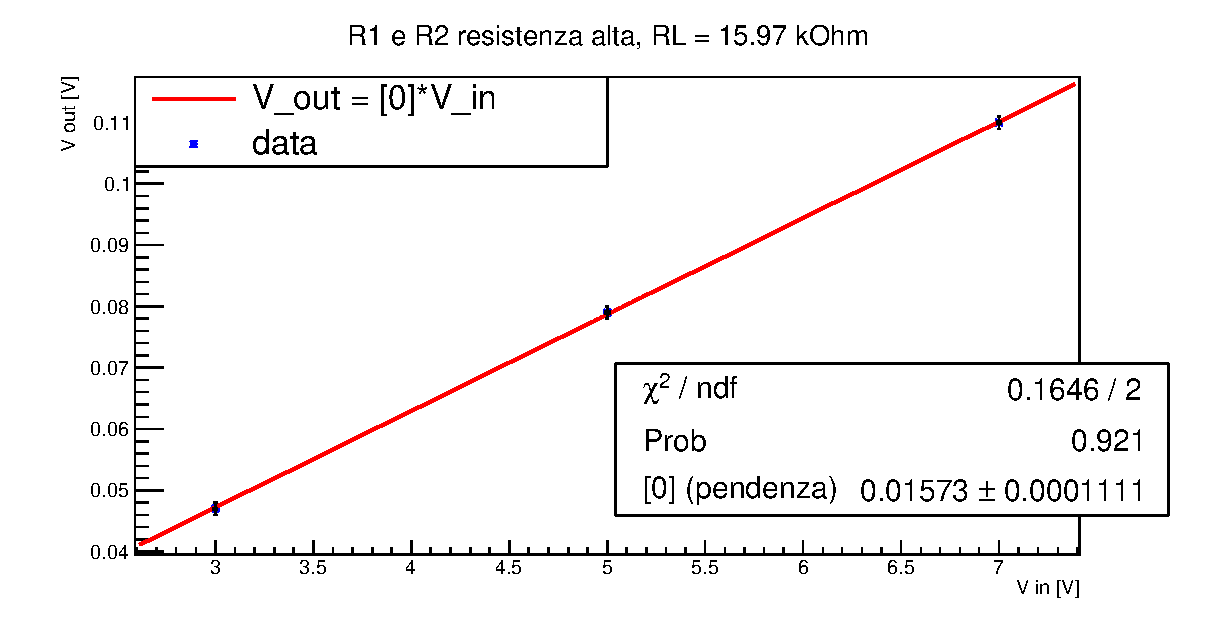
\includegraphics[scale=.7]{Grafici/C1_P2_partResHigh2.eps}
    \end{figure}
    
    \begin{figure}[H]
    \centering
    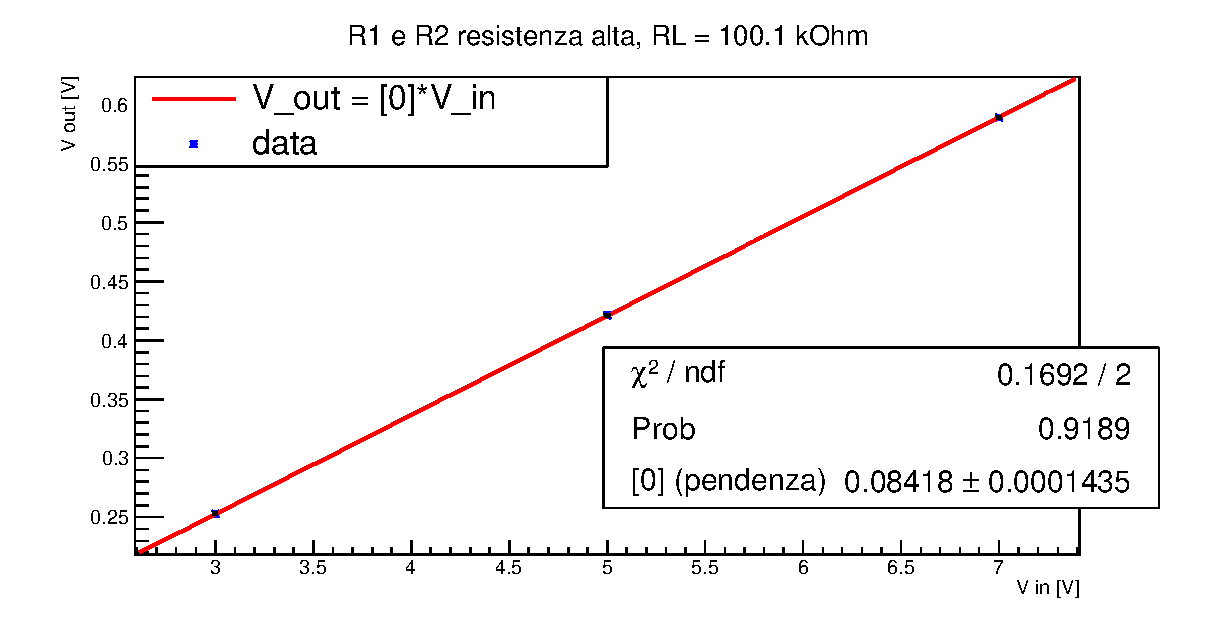
\includegraphics[scale=.7]{Grafici/C1_P2_partResHigh3.eps}
    \end{figure}
    %
    %
    Si è dunque verificato che:
    \begin{itemize}
        \item La caduta di tensione in $R_L$  dipende da $R_L$. Infatti a parità di $V_{in}$, cambiando $R_L$ il $V_{out}$ cambia.
        \item Non è vero che $V_{out} = 0.5 \cdot V_{in}$.
    \end{itemize}
%    
\subsubsection{Approfondimento: Potenza massima trasferibile}
    % Dati resistenze
    Si è tolta $R_2$ dal circuito.\\
    Per la misura di $R_g$ abbiamo utilizzato una resistenza $R_1$ da $10.1 \Omega$, e ricavato $R_g$ da
    $$Rg = \frac{fem-V}{I} = 1.4 \Omega $$
    %%manca errore Rg
    con $fem$ = forza elettromotrice erogata da generatore,
    $V$ = Differenza di potenziale misurata ai capi del resistore, $I$ = corrente che scorre attraverso il circuito.\\
    $R_g$ espresso come media delle misure e errore calcolato con le formule di propagazione.\\
%
    % tabella misura Rg
       \begin{table}[H]
    \centering
    \caption{Misura di $R_g$}
    \begin{tabular}{|c|c|c|c|}
    \hline
        $fem$ & Tensione (V) & Corrente (A) & Rg \\ \hline
        V & V & A & $\Omega$ \\ \hline
        $\pm$0.01 & $\pm$0.001 & $\pm$ 0.001 & 0.02 \\ \hline
        3.00 & 2.626 & 0.267 & 1.401 \\ 
        2.50 & 2.189 & 0.222 & 1.401 \\ 
        2.00 & 1.756 & 0.178 & 1.371 \\ 
        1.50 & 1.323 & 0.135 & 1.311 \\ \hline
    \end{tabular}
    \label{}
    \end{table}
%
    Per la misura della massima potenza dissipabile su $R_L$ abbiamo utilizzato una resistenza $R_1= 149 k\Omega$, nota $R_g = 0.0014 k\Omega$, e una $fem$ da $7.5 V$. \\
 %
    La previsione teorica del massimo di potenza dissipata in $R_L$ è ottenuta massimizzando la funzione
    $$P=I^2\cdot R_{L} = \frac{fem^2 R_L}{(R_g + R_1 + R_L)^2} $$
    dove la corrente è stata ricavata dall'equazione del circuto:   
    $$fem- IR_g = IR_1 + I R_L \Rightarrow I = fem / (R_g+R_1+R_L)$$
    ponendo $\frac{\partial P}{\partial R_L} = 0$, si trova:
    $$ R_L max = R_1+R_g = 149  k\Omega$$
%
    Le misure indicano un massimo di potenza in prossimità di $R_L = 150 k\Omega$.\\
    %
    Di seguito il grafico che mostra la curva della potenza dissipata in $R_L$, e una linea verticale che segna il massimo teorico, che si trova abbastanza vicino al massimo della curva. Abbiamo quindi verificato quanto dimostrato in teoria.\\   
    % Grafico RL / potenza
    \begin{figure}[H]
    \centering
    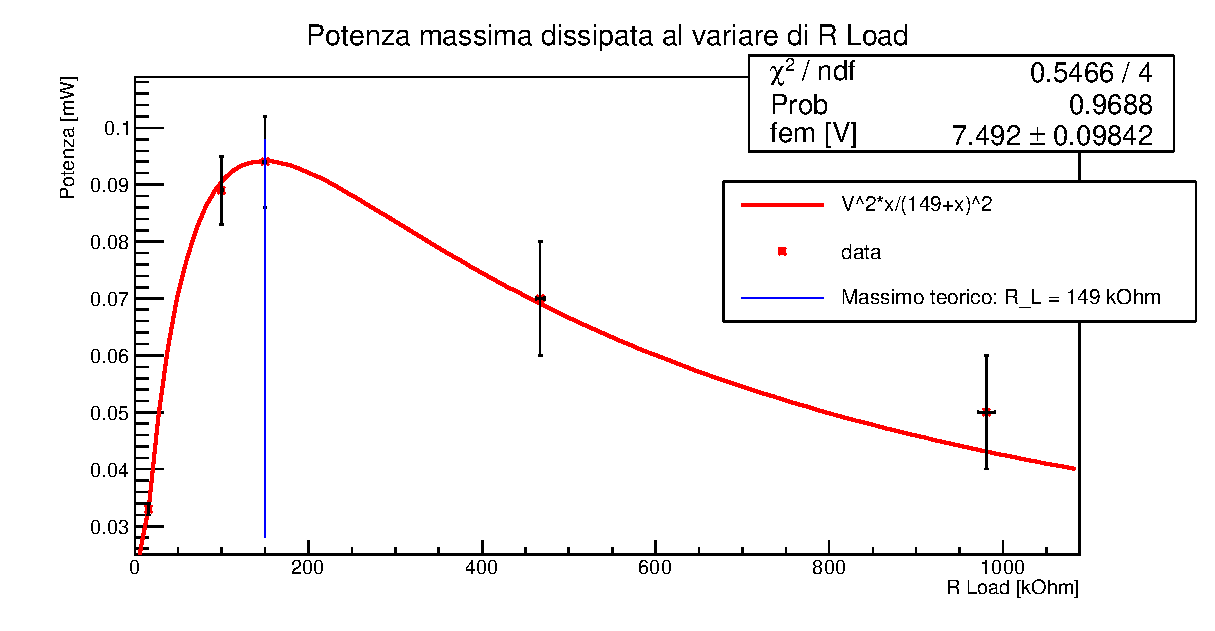
\includegraphics[scale=.7]{Grafici/C1_P2_maxPower.eps}
    \caption{Grafico Resistenza-Potenza trasferita}
    \label{fig:C1_P2_maxPower}
    \end{figure}
    

    
    
    

\newpage

\subsection{Parte 3 }
\subsubsection{Diodo led}


\begin{table}[H]
\begin{center}
\begin{tabular}{|c|c|c c c c c c c c c|}
    \hline
    unit & +/- \% & \multicolumn{9}{c|}{Osservazioni}\\ 
    \hline
    V & 0.01 & 1.85 & 2.20 & 2.25 & 2.30 & 2.35 & 2.40 & 2.45 & 2.50 & 2.55 \\ 
    mA & 1 & 0.01 & 0.01 & 0.01 & 0.02 & 0.06 & 0.15 & 0.33 & 0.54 & 0.88 \\ 
    \hline
    V & 0.01 & 2.60 & 2.65 & 2.70 & 2.75 & 2.80 & 2.85 & 2.90 & 2.95 & 3.00 \\ 
    mA & 1 & 1.32 & 1.93 & 2.54 & 3.33 & 4.11 & 5.08 & 6.02 & 7.45 & 8.45 \\ \hline
    \end{tabular}
    \end{center}
    \caption{Diodo led. Risposta corrente [mA] per tensione [V].}
    \label{C1_P3_dati}
\end{table}


Il grafico è stato fittato solo a partire da $V = 2.4 V$, ossia da dove parte la curvatura caratteristica.\\
La formula del fit è
$$ I = I_0 \cdot (e^{qV/gkt} -1) + a\cdot V $$
Il termine $a$ indica che si è tenuto conto del fatto che il diodo è led, e quindi si comporta come se avesse in parallelo una resistenza).\\
$  \frac{q}{kt} \approx 38.6 $ e $g$ è una costante adimensionale caratteristica del diodo.

\begin{figure}[H]
\centering
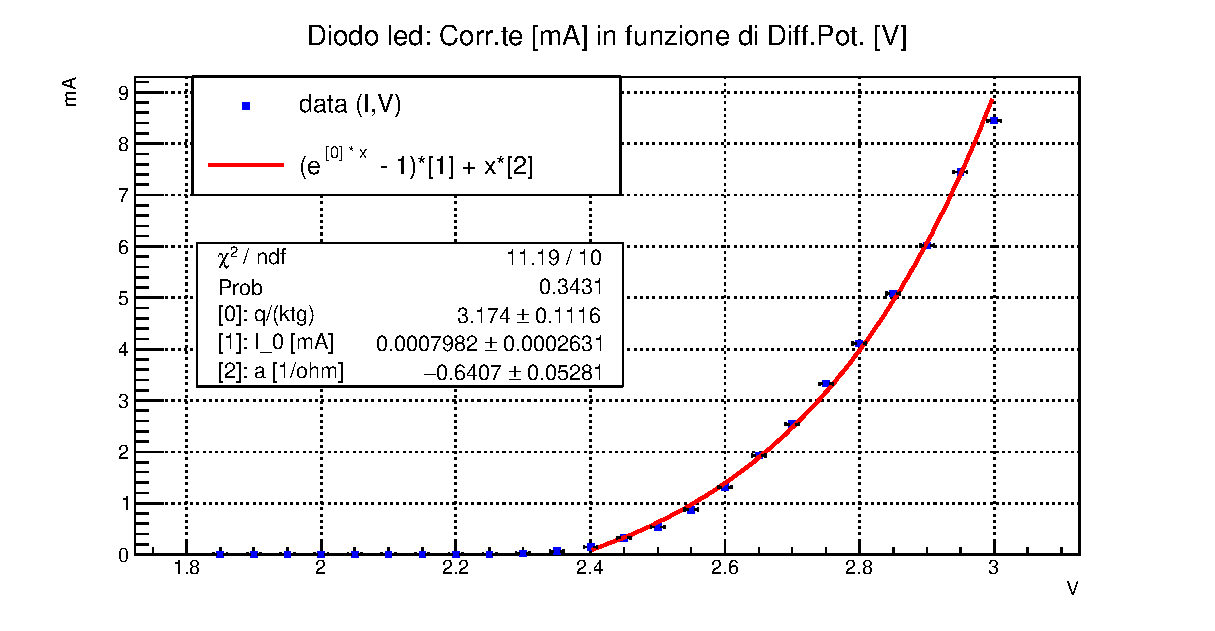
\includegraphics[scale=.7]{Grafici/C1_P3.eps}
\caption{
Risposta diodo led
}
\label{fig:C1_P3}
\end{figure}
%
%
Il chi quadro ridotto è molto vicino a 1, il che indica un buon adattamento dei dati al fit.
\newpage





%%%%%%%%%%%%%%%%%%%%%%%%%%%%%%%%%%%%%%%%%%%%%%%%%%%%    
%%% C2

\section{Circuiti 2}

\subsection{Parte 1: Resistenza}
\subsubsection{Intervallo di funzionamento strumenti}
Scopo dell'esperienza è la valutazione dell'intervallo di corretta lettura di segnale per i multimetri. \\
Dato il circuito in corrente alternata di figura \ref{fig:C2_P1_circuito}, si misura la tensione ai capi di $Z$ con due strumenti: Multimetro palmare e Oscilloscopio. Si confrontano poi le letture per indivuduare le bande di frequenza in cui la lettura del multimetro risulta corretta.\\
%
Per le correnti viene eseguita la doppia misura con \textcolor{red}{ Multimetro} e Multimetro palmare e, analogamente, vengono confrontati i valori.\\
%
Vengono poi riportati in grafico i rapporti tra le misure effettuate con i due strumenti, $V_{multimetro}/V_{oscilloscopio}$ e $I_{multimetro}/I_{oscilloscopio}$, in funzione della frequenza $\omega$.
%
\paragraph{Nota} {
L'oscilloscopio fornisce letture picco-picco, cioè riporta la differenza di tensione/corrente tra un massimo e un minimo, che è il doppio dell'ampiezza dell'oscillazione di tensione/corrente. Occorre normalizzare per un fattore 1/2 la misura. \\
Il multimetro palmare fornisce letture in RMS, cioè riporta la radice della media quadratica della tensione/corrente sul periodo $T$. Supposta un'oscillazione sinusoidale, $ f(t) = A_0 \sin(\omega t)$, la media quadratica su $[0,T]$ è
    $$\langle f^2(t) \rangle = \frac{1}{T} \; \int_0^{T} A_0^2 \cos^2(\omega t) \mathrm{d}t = \frac{1}{2}A_0^2$$
e la radice:
    $$ \sqrt{ \langle f^2(t) \rangle } = \frac{A_0}{\sqrt{2}}$$
occorre quindi normalizzare il valore per un fattore $\sqrt{2}$.\\
Si è scelto di riportare tutte le quantità in picco-picco.\\
%
\begin{figure}[H]
\centering
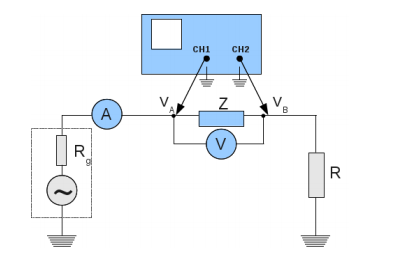
\includegraphics[scale=.6]{Grafici/C2_P1_circuito.png}
\caption{Circuito utilizzato.}
\label{fig:C2_P1_circuito}
\end{figure}

\paragraph{Dati e risultati}{
Ddp generata $V_{a}=9.0\pm0.2$ $V$.\\
Resitore per conversione in corrente del segnale in uscita dall'oscilloscopio $R=990\pm20$ $\Omega$. Si riporta in grafico il logaritmo della frequenza $\nu$.
%
    \begin{figure}[H]
        \centering
        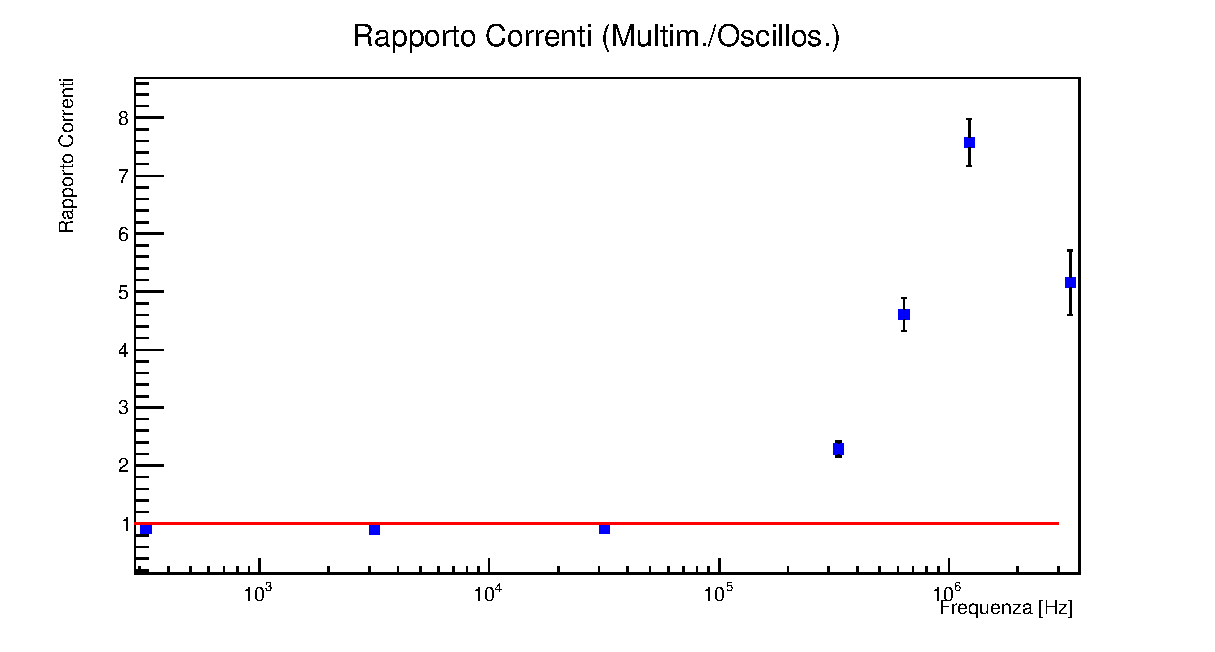
\includegraphics[scale=.6]{Grafici/C2_P1_trueRMS_I.eps}
        \caption{
        Rapporto delle misure di corrente (picco-picco)
        eseguite con multimetro e oscilloscopio per la verifica dell'intervallo di TRUE RMS.
        }
        \label{fig:C2_P1_trueRMS_I}
    \end{figure}
    
    \begin{figure}[H]
        \centering
        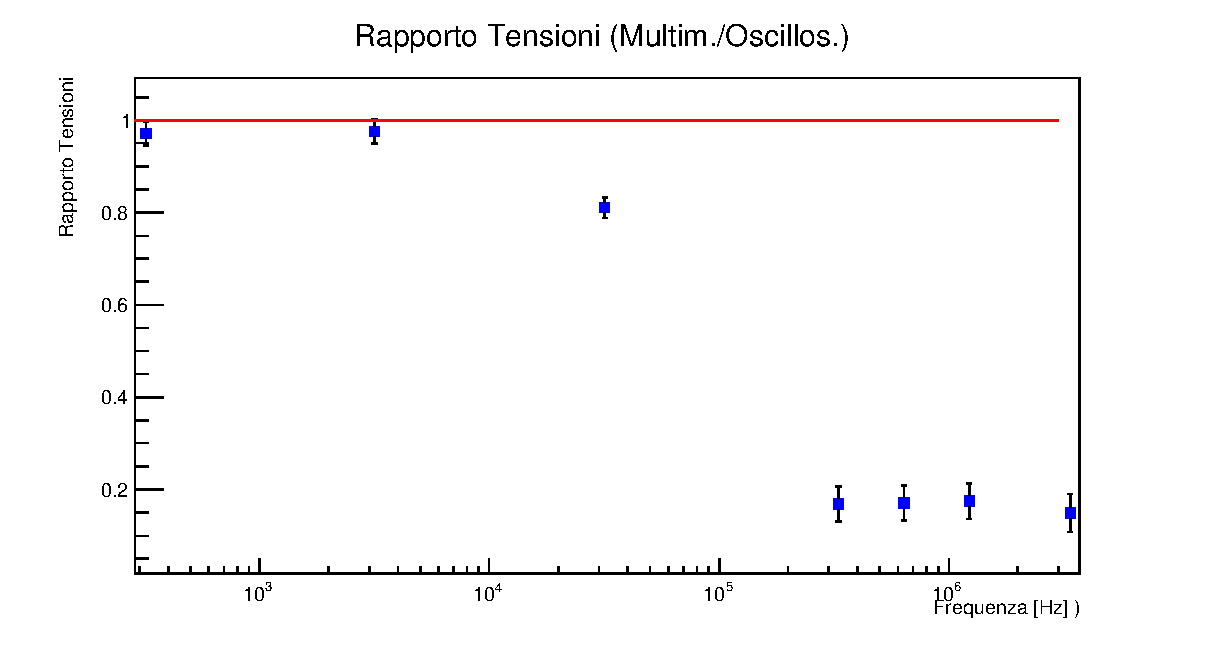
\includegraphics[scale=.6]{Grafici/C2_P1_trueRMS_V.eps}
        \caption{
        Rapporto delle misure di voltaggio (picco-picco) eseguite con multimetro e oscilloscopio per la verifica dell'intervallo di TRUE RMS.
        Usato lo stesso circuito della fig. \ref{fig:C2_P1_trueRMS_I}.
        }
        \label{fig:C2_P1_trueRMS_V}
    \end{figure}
    
}%}

\paragraph{Conclusioni}{
Si può notare che l'intervallo di funzionamento ottimale del multimetro palmare comprende le frequenze fino all'ordine dei $10 kHz$.
}

\subsubsection{Impedenza}
Scopo dell'esperienza è valutare modulo e fase dell'impedenza per un resistore in un circuito solo resistivo.\\
Per un componente resistivo, l'impedenza ha solamente parte reale con $Z=R_Z$, quindi si ha $Mod(Z) = R_Z$ e $Arg(Z) = 0 $. Per determinare il valore della resistenza, si applica la legge di Ohm, dove si indica con $Z$ l'impedenza (resistenza) relativa al resistore da misurare e con $R$ la resistenza di prova per la misura della corrente ($R=1kOhm$). 
    $$ Z = V/I = \frac{V_{b-a} }{V_b/R} $$
    %
Noto il valore di $Z=15.97 k\Omega$ (misurato con multimetro), i dati riportano (si osservi l'ultima riga della tabella \ref{tab:C2_P1_trueRMS} per i valori della fase $\Delta \phi(V_ab - I_b)$.
%
    \begin{figure}[H]
        \centering
        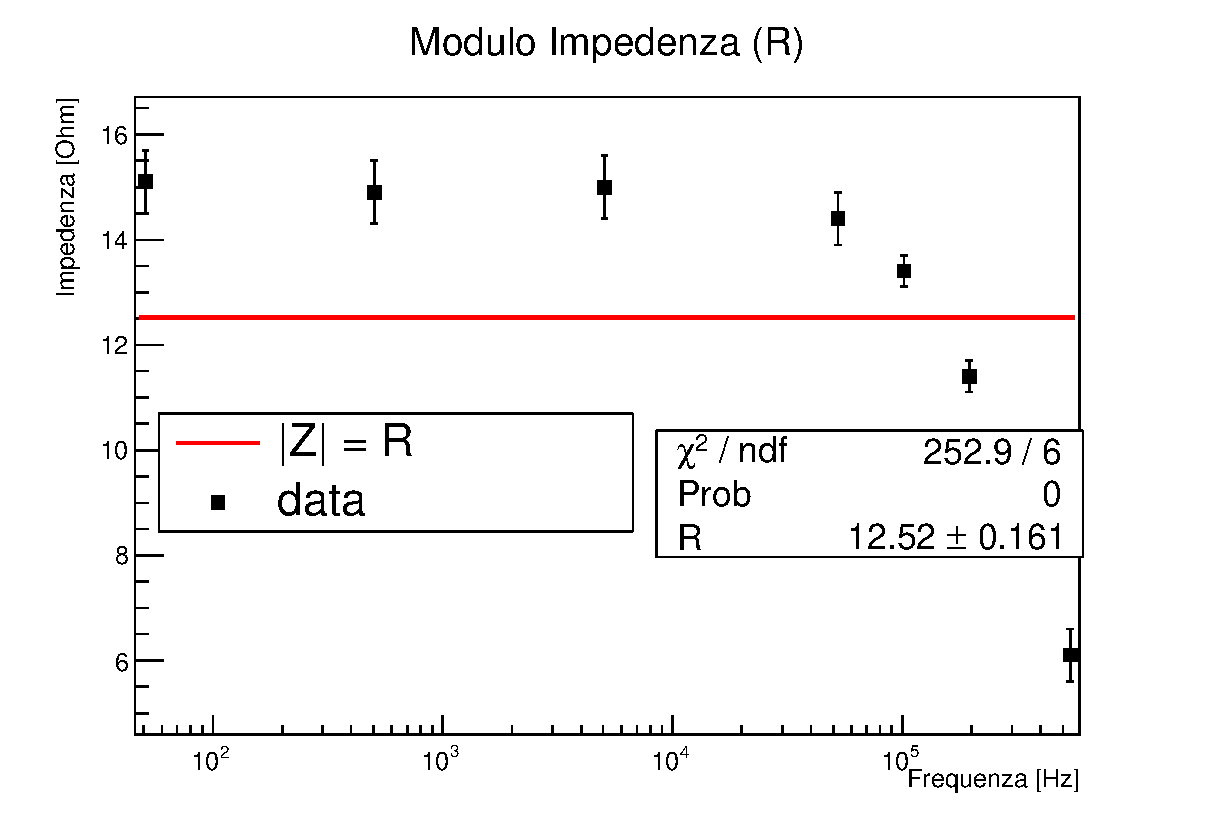
\includegraphics[scale=.7]{Grafici/C2_P1_impedenzaR.eps}
        \caption{Dati relativi al modulo dell'impedenza}
    \end{figure}
%
\paragraph{Considerazioni}{Per quanto riguarda il modulo dell'impedenza, dal fit risulta $ 12.5 \pm 0.2 k\Omega$, ben lontano dal valore misurato con il multimetro, mentre per la fase si osserva che assume valori non nulli ad alte frequenze. Si attribuisce l'effetto a eventuali componenti non resistive degli strumenti di misura, o a malfuzionamento.}
\subsubsection{Tabelle dati}
    \begin{table}[H]
\begin{center}
\begin{tabular}{|c|c|c|c|c|c|c|c|c|}
\hline
\multicolumn{9}{|c|}{ \textbf{Generatore di funzioni} } \\ \hline
%
Freq & Hz $\pm 2$\% & 50.8 & 504 & 5.10 k & 52.6 k & 101 k & 195 k & 537 k \\ \hline
%
\multicolumn{9}{c}{}\\
\hline
\multicolumn{9}{|c|}{ \textbf{Multimetro palmare - Fluke 115} }\\ \hline
V rms & V & 2.86 & 2.87 & 2.45 & 0.5 & 0.5 & 0.5 & 0.4 \\ 
 & $\pm$ err & 0.01 & 0.01 & 0.01 & 0.1 & 0.1 & 0.1 & 0.1 \\ \hline
V pp & V & 8.09 & 8.12 & 6.93 & 1.4 & 1.4 & 1.4 & 1.1 \\ 
 & $\pm$ err & 0.03 & 0.03 & 0.03 & 0.3 & 0.3 & 0.3 & 0.3 \\
%
\hline
\multicolumn{9}{c}{}\\
\hline
\multicolumn{9}{|c|}{ \textbf{Multimetro - HP 34401A} }\\ \hline
I rms & $\mu$ A & 181.0 & 181.0 & 188.0 & 474 & 1020 & 1920 & 2210 \\ 
 & $\pm$ err & 0.1 & 0.1 & 0.1 & 1 & 10 & 10 & 10 \\ \hline
I pp & $\mu$ A & 512 & 511.8 & 530.6 & 1341 & 2890 & 5430 & 6250 \\
 & $\pm$ err & 0 & 0.3 & 0.3 & 3 & 30 & 30 & 30 \\\hline
\multicolumn{9}{c}{}\\
\hline
\multicolumn{9}{|c|}{ \textbf{Oscilloscopio - Tektronik tds 220} }\\ \hline
Va & V & 8.9 & 8.9 & 9.1 & 9.0 & 8.9 & 8.8 & 8.8 \\ 
 & $\pm$ err & 0.2 & 0.2 & 0.2 & 0.2 & 0.2 & 0.2 & 0.2 \\ \hline
Vb & V & 0.55 & 0.56 & 0.57 & 0.58 & 0.62 & 0.71 & 1.2 \\ 
 & $\pm$ err & 0.02 & 0.02 & 0.02 & 0.02 & 0.02 & 0.02 & 0.1 \\ \hline
$V(b-a)$ & V & 8.3 & 8.3 & 8.6 & 8.4 & 8.3 & 8.1 & 7.6 \\ 
 & $\pm$ err & 0.2 & 0.2 & 0.2 & 0.2 & 0.2 & 0.2 & 0.2 \\ \hline
$ Ib = Vb/R $ & $\mu$ A & 0.56 & 0.57 & 0.58 & 0.59 & 0.63 & 0.72 & 1.21 \\
 & $\pm$ err\% & 6\% & 6\% & 6\% & 5\% & 5\% & 5\% & 10\% \\ 
%
\hline
\multicolumn{9}{c}{}\\
\hline
%
\multicolumn{9}{|c|}{\textbf{Differenze di fase}}\\\hline
$\Delta\phi' (Va-Vb) $  & ns        & 0 & 0 & 0 & 800 & 600 & 440 & 250 \\
                        & $\pm$err  & 0 & 0 & 0 & 100 & 100 & 40  & 10  \\
\hline
$\Delta\phi (Vab - Ib)$ & ns        & 0 & 0 & 0 & 1400 & 1400 & 1200 & 710 \\ 
                        & $\pm$err  & 0 & 0 & 0 & 200  & 100  & 40   & 10  \\
\hline

\end{tabular}
\end{center}
\caption{
Dati relativi ai grafici delle figure \ref{fig:C2_P1_trueRMS_I} e \ref{fig:C2_P1_trueRMS_V}.
Resitore $R=990\pm20$ $\Omega$.
$T=1/\nu$ indica il periodo.
}
\label{tab:C2_P1_trueRMS}
\end{table}

\newpage

\subsection{Parte 2: Capacità}
%%%%%%%%%%%%%%%%%%%%%%%%%%%%%%%%%%%%%%%%%%%%%%%%%%%%%%%%%%%%%%%%%%%%%%%%%%%%%%%% INIZIO %%%%%%%%%%%%%%%%%%%%%%%%%%%%
Scopo dell'esperienza è la misura dell'impedenza e della funzione di trasferimento ai capi di una capacità. Come verrà dimostrato nella sezione \ref{sec:C3_P2-1}, l'impedenza per una capacità è:  $Z_c = \frac{1}{\omega C} \; e^{-j\pi/2}$
\\
%
%%%%%%%%%%%%%%%%%%%%%%%%%%%%%%%%%%%%%%%%%%%%%%%%%%%%%%%%%%%%%%%%%%%%%%%%%%%%%%%% FDT %%%%%%%%%%%%%%%%%%%%%%%%%%%%%%%
%
\subsubsection{Funzione di trasferimento per C}
La funzione di trasferimento ai capi del componente C, $V_{b-a}/V_a$, è:
$$ H(\omega) = \frac{ V_{b-a} }{V_a} = \frac{Z_CI}{Z_{tot}I} = \frac{\frac{1}{j\omega C}}{R + \frac{1}{j\omega C}} = \frac{1}{1+j\omega CR} $$
%
per cui, modulo e argomento sono:
%
$$ Mod(H) = \frac{1}{\sqrt{ 1+(\omega R_{tot} C)^2} } \quad e \quad Arg(H) = \arctan(-\omega R_{tot}C) $$
%
Con $R_{tot} =  R + r_{gen} = 14900 \pm 200 \Omega $.
\begin{figure}[H]
    \centering
    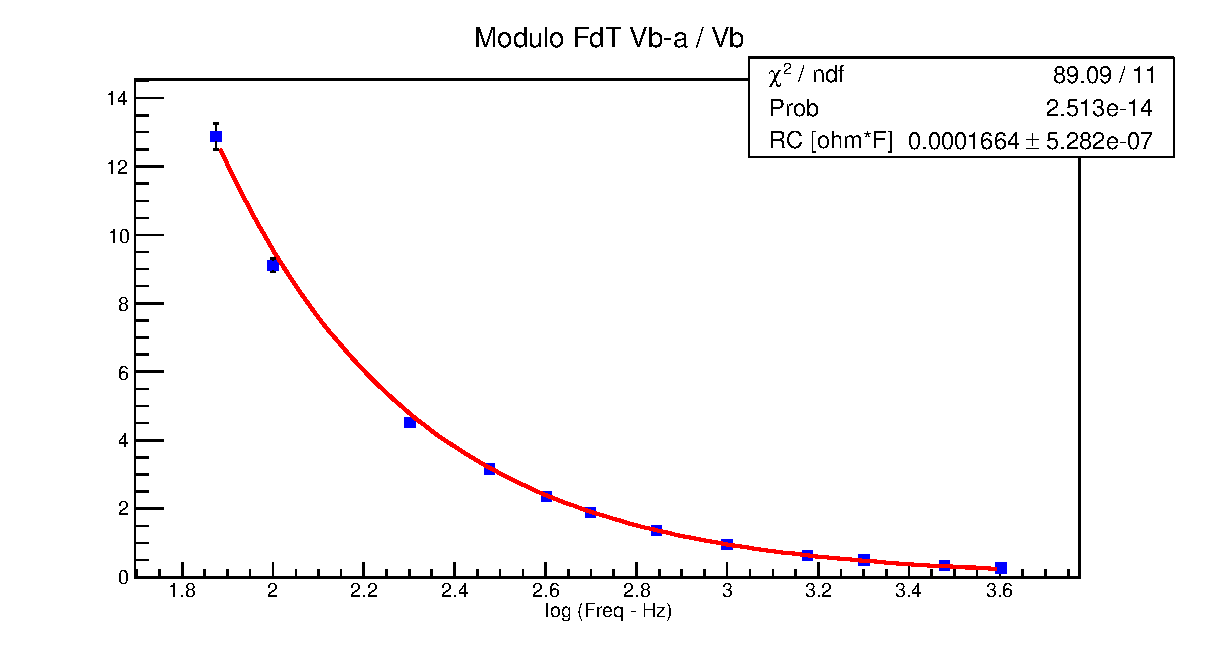
\includegraphics[scale=.6]{Grafici/C2_P2_ModFdt1_.eps}
    \caption{
        Modulo funzione di trasferimento $ \tfrac{Vba}{Vb} $.
         Capacità valore nominale $11$ $nF$
    }
    \label{fig:C2_P2_ModFdt1}
\end{figure}
%
\begin{figure}[H]
    \centering
    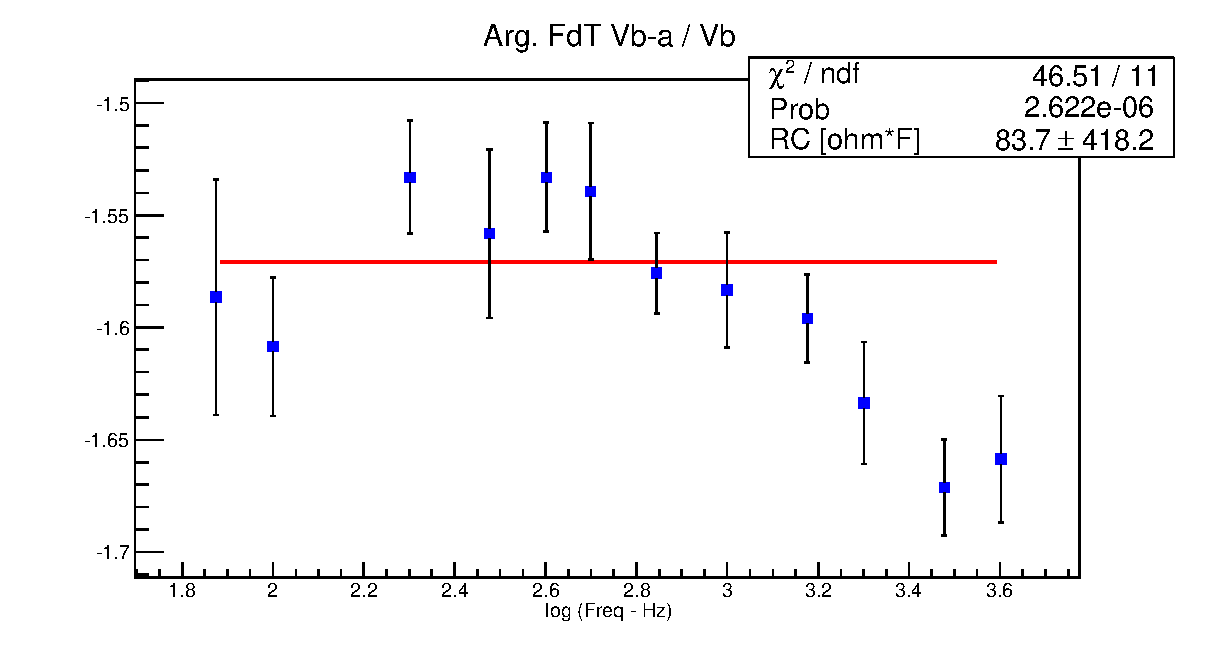
\includegraphics[scale=.6]{Grafici/C2_P2_ArgFdt1_.eps}
    \caption
    {
        Argomento funzione di trasferimento $ \tfrac{Vba}{Vb} $.
        Capacità valore nominale $11$ $nF$
    }
    \label{fig:C2_P2_ArgFdt1}
\end{figure}
%%%%%%%%%%%%%%%%%%%%%%%%%%%%%%%%%%%%%%%%%%%%%%%%%%%%%%%%%%%%%%%%%%%%%%%%%%%%%%%% IMPEDENZA %%%%%%%%%%%%%%%%%%%%%%%%%
\subsubsection{Impedenza per C}
L'impedenza per C vale $Z_C = \tfrac{1}{j\omega C}$ di modulo $ Mod(Z) = \tfrac{1}{\omega C}$ e fase $Arg(Z)= \arctan(- 1/ \omega C)$
%	C: 26200 +/- 193 nF
\begin{figure}[H]
    \centering
    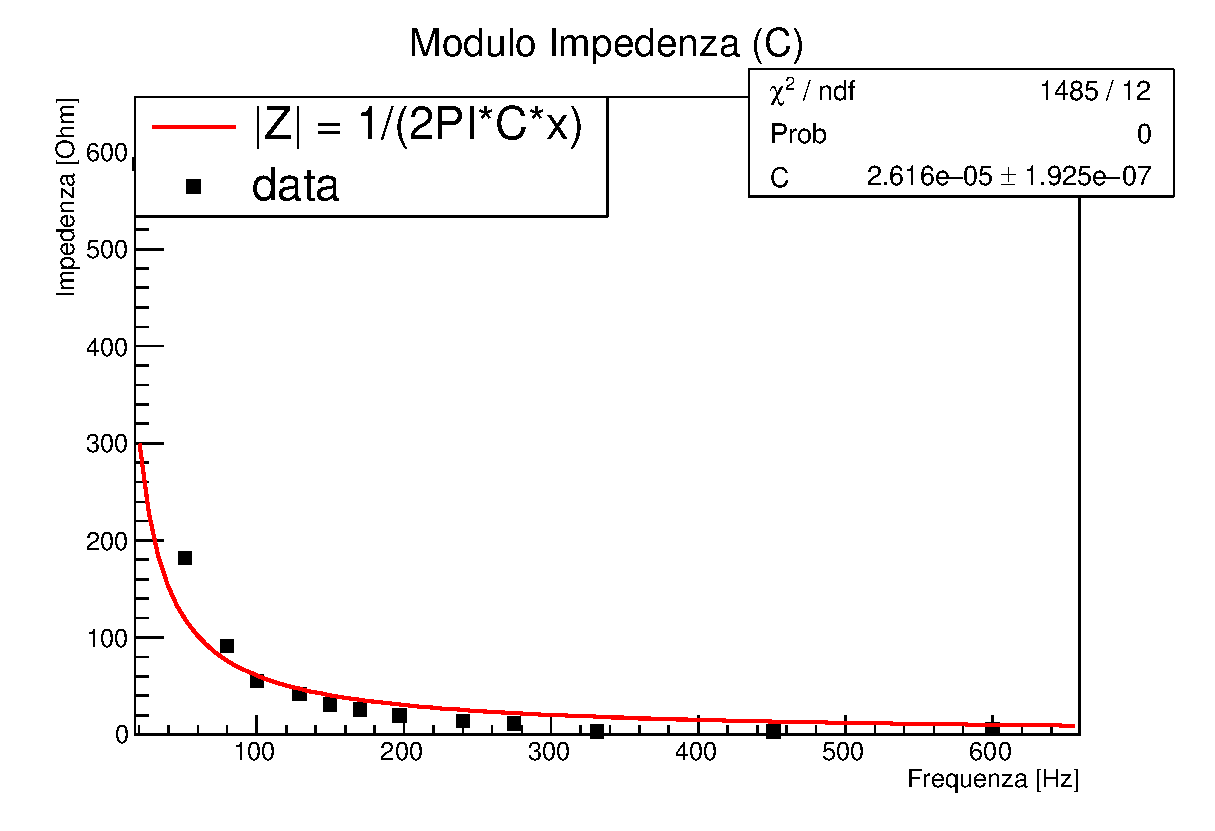
\includegraphics[scale=.7]{Grafici/C2_P2_impedenzaC.eps}
    \caption{Modulo dell'impedenza per C}
    \end{figure}

\begin{figure}[H]
    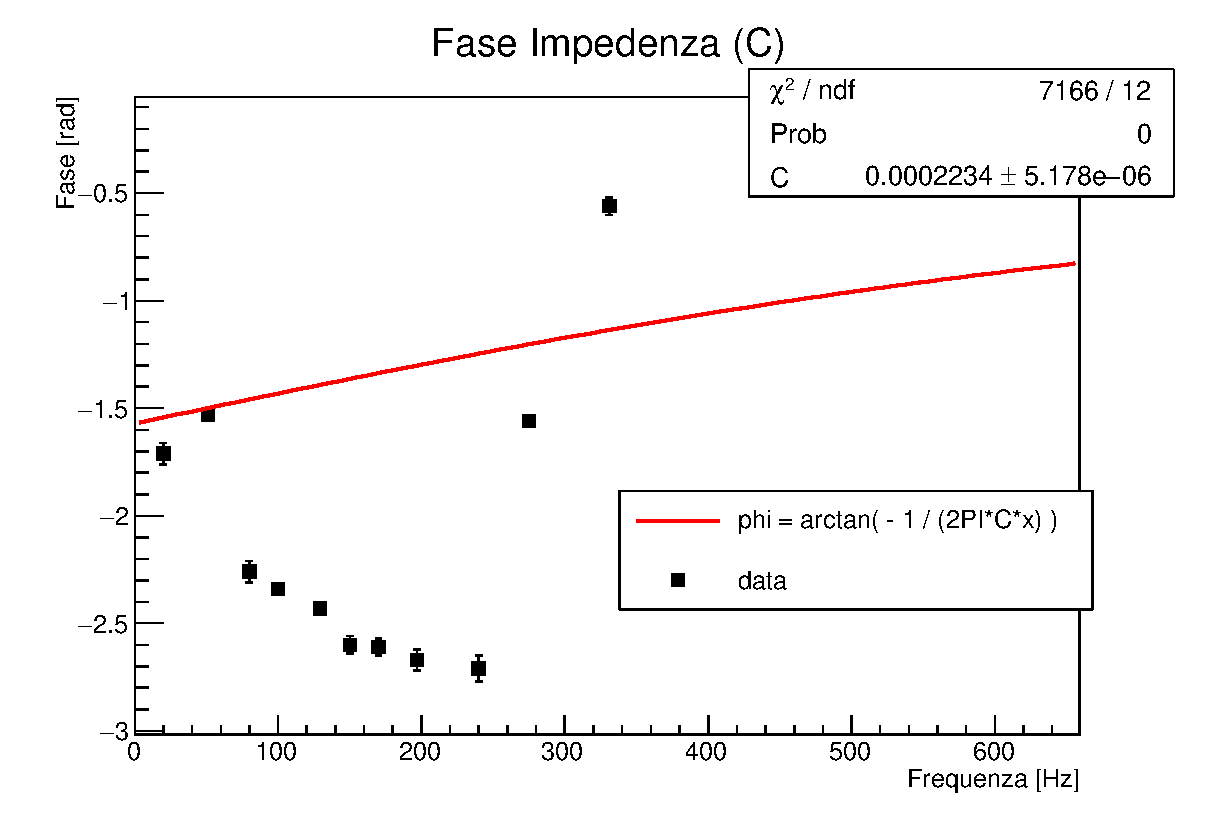
\includegraphics[scale=.7]{Grafici/C2_P2_impedenzaFaseC.eps}
    \caption{Fase dell'impedenza per C}
\end{figure}
\paragraph{Considerazioni}{I risultati dei fit producono valori di C non attendibili, considerando i $\chi^2$ ottenuti.}
%%%%%%%%%%%%%%%%%%%%%%%%%%%%%%%%%%%%%%%%%%%%%%%%%%%%%%%%%%%%%%%%%%%%%%%%%%%%%%%%
\subsubsection{Funzione di trasferimento $V_b/V_a$}
La funzione di trasferimento ai capi della resistenza R è:
  $$ H(\omega) = \frac{V_b}{V_a} = \frac{Z_RI}{Z_{tot}I} =  \frac{R \frac{V_a}{R+Z_C}}{V_a} =
  \frac{R}{R + \frac{1}{j\omega C} } = \frac{1}{j\omega CR + 1} $$
e quindi:
  $$ Mod(H) = \frac{\omega C R}{\sqrt{1 + (\omega CR)^2}} \quad \mathrm{e} \quad Arg(H) = \arctan(\frac{1}{\omega CR})$$
%
\begin{figure}[H]
    \centering
    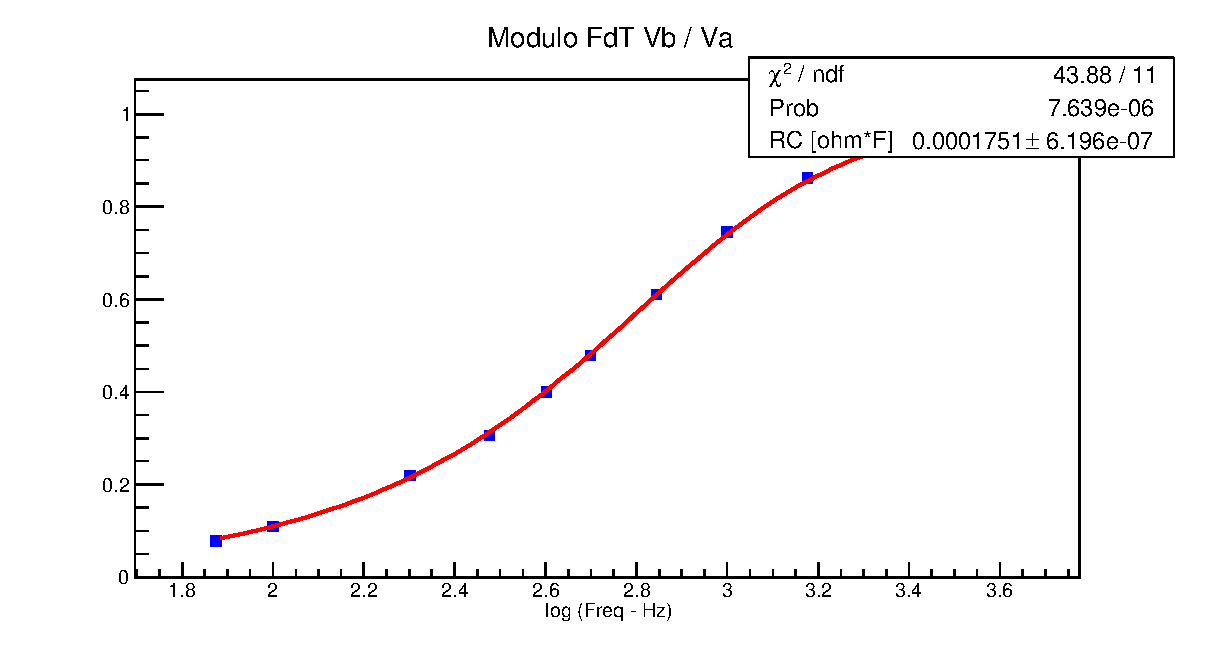
\includegraphics[scale=.6]{Grafici/C2_P2_ModFdt2_.eps}
    \caption
    {
        Modulo funzione di trasferimento $ \tfrac{Vb}{Va} $.
    }
    \label{fig:C2_P2_ModFdt2}
\end{figure}
%
\begin{figure}[H]
    \centering
    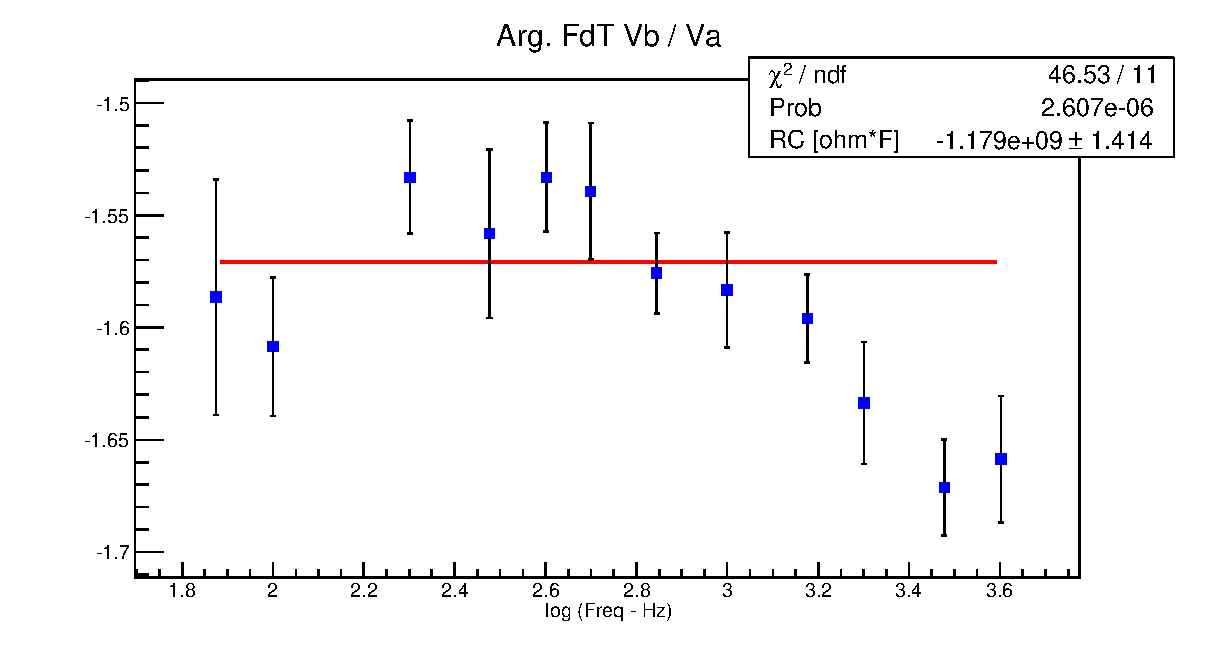
\includegraphics[scale=.6]{Grafici/C2_P2_ArgFdt2_.eps}
    \caption
    {
        Argomento funzione di trasferimento $ \tfrac{Vb}{Va} $.
        Resistenza totale $ R + r_{gen} = 14870 + 50 \pm 150 \Omega $.
        Capacità valore nominale $11$ $nF$.
    }
    \label{fig:C2_P2_ArgFdt2}
\end{figure}
%%%%%%%%%%%%%%%%%%%%%%%%%%%%%%%%%%%%%%%%%%%%%%%%%%%%%%%%%%%%%%%%%%%%%%%%%%%%%%%%%% DATI %%%%%%%%%%%%%%%%%%%%%%%%%%%%
\subsubsection{Dati}
\begin{table}[H]
\begin{center}
\begin{tabular}{|c|c|c|c|c|}
\hline
\multicolumn{ 2}{|c|}{Fdt} & $R_{tot}C$ & $C$ & $\chi^{2}$ \\ \hline
\multicolumn{ 2}{|c|}{   } & $\omega\cdot nF$ & $nF$ &  \\ \hline

\multicolumn{ 1}{|c|}{$Vba/Vb$} & mod 
& $166400\pm500$  & $11.15\pm1.3\%$ & 89/11  \\

\multicolumn{ 1}{|c|}{} & arg & - & -  &  \\ \hline

\multicolumn{ 1}{|c|}{$Vb/Va$} & mod 
& $175100\pm619$ & $11.73\pm1.3\%$ & 44 / 11  \\

\multicolumn{ 1}{|c|}{} & arg & - & - &  \\ \hline

\end{tabular}
\end{center}
\caption{
Riepilogo risultati fit.
Resistenza totale $ R + r_{gen} = 14870 + 50\pm 150$ $\Omega$.
}
\label{C2_P2_risultati}
\end{table}

\begin{table}[H]
\begin{center}
\begin{tabular}{|r|r|r|r|r|r|r|r|}
\hline
\multicolumn{1}{|l|}{Freq} & \multicolumn{1}{l|}{Va} & \multicolumn{1}{l|}{Vb} & \multicolumn{1}{l|}{Vb-a} & \multicolumn{1}{l|}{-Fase (CH2)} & \multicolumn{1}{l|}{err-(CH2)} & \multicolumn{1}{l|}{-Fase (CH1)} & \multicolumn{1}{l|}{err-(CH1)} \\ \hline
\multicolumn{1}{|l|}{Hz} & \multicolumn{1}{l|}{V} & \multicolumn{1}{l|}{V} & \multicolumn{1}{l|}{V} & \multicolumn{1}{l|}{$\mu$s} & \multicolumn{1}{l|}{$\mu$s} & \multicolumn{1}{l|}{$\mu$s} & \multicolumn{1}{l|}{$\mu$s} \\ \hline
\multicolumn{1}{|c|}{$\pm$ 1} & \multicolumn{1}{c|}{$\pm$ 0.08} & \multicolumn{1}{c|}{$\pm$ 0.08} & \multicolumn{1}{c|}{$\pm$ 0.16} & \multicolumn{1}{l|}{} & \multicolumn{1}{c|}{$\pm$ } & \multicolumn{1}{l|}{} & \multicolumn{1}{c|}{$\pm$ } \\ \hline
75 & 10.2 & 0.80 & 10.3 & 3300 & 200 & 6400 & 200 \\ \hline
100 & 10.2 & 1.12 & 10.2 & 2,440 & 80 & 4800 & 80 \\ \hline
200 & 10.2 & 2.24 & 10.1 & 1,280 & 40 & 2340 & 40 \\ \hline
300 & 10.2 & 3.12 & 9.84 & 840 & 40 & 1500 & 40 \\ \hline
400 & 10.2 & 4.08 & 9.60 & 640 & 20 & 1090 & 20 \\ \hline
500 & 10.2 & 4.88 & 9.20 & 510 & 20 & 850 & 20 \\ \hline
700 & 10.1 & 6.16 & 8.40 & 356 & 8 & 560 & 8 \\ \hline
1000 & 10.3 & 7.68 & 7.36 & 248 & 8 & 372 & 8 \\ \hline
1500 & 10.3 & 8.88 & 5.68 & 164 & 4 & 220 & 4 \\ \hline
2000 & 10.2 & 9.36 & 4.64 & 120 & 4 & 158 & 4 \\ \hline
3000 & 10.2 & 9.92 & 3.36 & 78 & 2 & 96 & 2 \\ \hline
4000 & 10.2 & 10.0 & 2.64 & 59 & 2 & 68 & 2 \\ \hline
\end{tabular}
\end{center}
\caption{
Dati relativi alle figure
\ref{fig:C2_P2_ModFdt1}
\ref{fig:C2_P2_ArgFdt1}
\ref{fig:C2_P2_ModFdt2}
\ref{fig:C2_P2_ArgFdt2}.
Condensatore valore nominale $11$ $nF$.
Resistore $14870\pm 150$ $ohm$.
}
\label{C2_P2_cond1}
\end{table}



\newpage





%%%%%%%%%%%%%%%%%%%%%%%%%%%%%%%%%%%%%%%%%%%%%%%%%%%%    
%%% C3

%\section{Circuiti 3}

%\subsection{Teoria: misure di impedenza in circuiti RC e RL in corrente alternata}

Consideriamo un circuito nel quale tensione e corrente variano nel tempo secondo una legge di tipo sinusoidale $V(t)=V_0 \cos(\omega t)$ ed $I(t)=I_0 \cos(\omega t)$. Consideriamo elementi circuitali resistivi (R), capacitivi (C) e induttivi (L) ed andiamo ad analizzare l'equazione caratteristica di ciascun componente per determinare l'espressione della differenza di potenziale ai capi di esso.\\\\
%
\textbf{Resistenze}:
L'equazione caratteristica di un resistore attraversato dalla corrente $I_0\cos(\omega t)$ è: 
    $$V_R (t) = RI(t) = RI_0 \cos(\omega t)$$
si nota quindi che ai capi di un resistore, la differenza di potenziale e la corrente sono in fase, e che tra le ampiezze sussiste la relazione:  
    $$V_0 = RI_0$$
Si osserva inoltre che non si ha alcuna dipendenza dalla pulsazione $\omega$\\\\
%
\textbf{Capacità}:
La capacità è definita come $C = Q/V_C$, dove $Q$ è la carica accumulata sul condensatore e $V_C$ è la tensione ai capi di esso. L'equazione del circuito, se viene applicata una tensione sinusoidale $V_C(t)=V_0 \cos(\omega t)$, diventa:
    $$Q(t) = CV_C(t) = CV_0 \cos(\omega t) $$
%    
La corrente quindi $I(t)=\mathrm{d}Q(t)/\mathrm{d}t$:
    $$I(t) = C \frac{\mathrm{d}V(t)}{\mathrm{d}t} = \omega C V_0 (-\sin \omega t) = \omega C V_0 \cos \left(\omega t + \frac{\pi}{2}\right) $$
%
La tensione ai capi di un condensatore in un circuito in cui scorre la corrente $I(t)=I_0 \cos(\omega t)$ si trova risolvendo l'equazione $I(t)=C\mathrm{d}V_L(t)/\mathrm{d}t$, ove si è posta la costante di integrazione (il potenziale $V_T$) a 0:
    $$V_C = \frac{1}{C} \!\cdot{}\!\!\!\! \int \!I(t) \mathrm{d}t = \frac{1}{\omega C} \!\cdot{}\! \sin(\omega t)  + V_T = \frac{1}{\omega C} \!\cdot{}\! \cos \left(\omega t - \frac{\pi}{2}\right)$$
%
La tensione risulta quindi sfasata di $-\pi/2$ rispetto alla corrente e il suo valore in modulo è:
    $$V_0 = \frac{1}{\omega C} I_0$$
%    
La quantità $1/\omega C$ si definisce \textit{reattanza} del condensatore.\\\\
%
\textbf{Induttanze}:
Per un elemento induttivo di resistenza trascurabile, ai capi del quale viene applicata una tensione alternata $V_L(t) = V_0 \cos(\omega t)$,  l'equazione del circuito è:

    $$ V_L(t) = L \frac{\mathrm{d}I(t)}{\mathrm{d}t} \Rightarrow \frac{\mathrm{d}I(t)}{\mathrm{d}t} = \frac{V_0 \cos(\omega t)}{L} \Rightarrow$$
    
    $$\Rightarrow I(t) = \frac{V_0}{\omega L}\sin(\omega t) = \frac{V_0}{\omega L}\cos\left(\omega t - \frac{\pi}{2}\right) $$

Dunque, la tensione ai capi di un induttore in cui scorre una corrente $I(t)= I_0\cos(\omega t)$ è:
    $$V_L =L\frac{\mathrm{d}I(t)}{\mathrm{d}t} =\omega L I_0 \cos\left(\omega t + \frac{\pi}{2}\right) $$
e in modulo:
$$V_0=\omega L I_0$$    
Tensione e corrente risultano sfasate di $+\frac{\pi}{2}$ e la reattanza dell'induttore è $\omega L$\\
%
\subsubsection{Simbolismo complesso}
Se per tensione e corrente utilizziamo la rappresentazione complessa $V(t)=V_0 e^{j(\omega t + \phi)}$ e $I(t)=I_0 e^{j\omega t}$, allora Tensione e corrente (complesse) risultano proporzionali.\\
%
Il coefficiente di proporzionalità tra tensione e corrente complesse è detto \textit{impedenza}, un numero complesso che racchiude gli effetti del circuito: il suo modulo indica il rapporto tra le ampiezze di V e I reali e la sua fase indica il loro sfasamento. 
    $$ Z = Z_0 e^{j\phi} $$  
\paragraph{Nota}{
        Indicheremo con $\phi$ lo sfasamento della tensione rispetto alla corrente. Cioè se $I(t)=I_0 \cos(\omega t)$ allora $V(t)=V_0\cos(\omega t + \phi)$}
    \\
Se rappresentato in forma algebrica $Z = R + jX$, la sua parte reale indica la componente resistiva del circuito e la sua parte immaginaria la componente reattiva (reattanza sopra definita è la parte immaginaria dell'impedenza).
    $$Z=R+jX$$
dove $j$ è l'unità immaginaria.\\
%
Il reciproco dell'impedenza è detto \textit{ammettenza}  $Y=1/Z$

Ripetendo i calcoli per i potenziali ai capi di R, C e L con il formalismo complesso, si trova che:
%
\begin{center}
\begin{tabular}{ l l l l l }
 $Z_R$ & $Z = R$ & $R \cdot{} \mathrm{exp}(j0)$ & $Z_0= R C$ & $\phi= 0$\\
 %
$Z_C$ & $Z = 1/j\omega C$ & $1/\omega C \cdot{} \mathrm{exp}(-j\pi/2)$ & $Z_0= 1/\omega C$ & $\phi= -\pi/2$\\  
 %
 $Z_L$ & $Z = j\omega L$ &  $\omega L \cdot{} \mathrm{exp}(j \pi/2)$   & $Z_0=\omega L$ & $\phi= \pi/2$
\end{tabular}
\end{center}
%
In circuiti composti da serie e parallelo di R, L, e C, si sommano impedenze in serie e ammettenze in parallelo con le consuete leggi di Kirchoff.\\
%
\subsubsection{Calcolo impedenze su circuiti RC e RL}
L'impedenza totale del circuito è $Z = \sum_{i=1}^n R_i = R + jX$. Il suo modulo è dato da $|Z| = \sqrt{R^2 + X^2}$ e la sua fase da $\phi = \arctan (X/R)$. Seguono calcoli dell'impedenza per circuito RC ed RL.\\\\
%
\textbf{Serie RC}
    $$Z = Z_R+Z_C = R + \frac{1}{j\omega C} = \sqrt{ R^2+\frac{1}{(\omega C)^2} } \cdot{} e^{j\phi} \rightarrow $$
    $$\rightarrow|Z|= \sqrt{ R^2+\frac{1}{(\omega C)^2} } \quad,\quad \phi = -\arctan \left(\frac{1}{\omega R C}\right)$$
Attendiamo dunque che a basse frequenze il circuito abbia un comportamento capacitivo (quindi che la fase dell'impedenza tenda a $-\pi/2$) e che ad alte frequenze abbia un comportamente resistivo (che la fase dell'impedenza tenda a 0).\\
Questo supporta l'intuizione in quanto per le basse frequenze il rapporto tra la costante di tempo del circuito e il periodo è molto basso. Ciò significa che in un periodo il numero di scariche della capacità (e quindi il flusso di carica nell'intervallo di tempo) è molto basso, e, nel limite di corrente continua, il circuito risulta aperto (non passa corrente attraverso C). La differenza di potenziale ai capi di C corrisponde al massimo di ampiezza della tensione. Come vedremo nella sezione successiva la funzione di trasferimento tende al valore 1.\\
Ad alte frequenze il rapporto tra il tempo caratteristico e il periodo dell'oscillazione è alto e la capacità ha numerose scariche in un periodo, permettendo un transito netto di corrente con una componente resistiva molto bassa. La tendenza è quindi quella di un cortocircuito, e la funzione di trasferimento tende a zero.

Se consideriamo anche la resistenza interna del generatore ($r_g$), nominalmente di $50 \Omega$, nel calcolo precedente è sufficiente sostituire il termine R alla somma $R + r_g$. L'impedenza diventa quindi:
 $$|Z|= \sqrt{ (R+r_g)^2+\frac{1}{(\omega C)^2} } \quad,\quad \phi = -\arctan (\frac{1}{\omega (R+r_g) C})$$
%
Di seguito le resistenze che abbiamo utilizzato e l'influenza della resistenza del generatore.
\begin{center}
    \begin{tabular}{|c c c|}\hline
            &                   & effetto $r_g$  \\
         R1 & 14870 $\Omega$    & 0.3\%      \\
         R2 & 677 $\Omega$      & 7\%   \\\hline
    \end{tabular}
    \label{tab:C3_P1_effetto_rg}
\end{center}
%
Per R2 ci aspettiamo che possa avere infuenza significativa\\

\textbf{Serie RL}
$$ Z = Z_R + Z_L = R + j\omega L = \sqrt{R^2+(\omega L)^2} \cdot{} e^{j\phi} $$
$$ |Z| = \sqrt{R^2+(\omega L)^2} \quad , \quad \phi = \arctan \left( \frac{\omega L}{R}\right) $$
Attendiamo dunque che a basse frequenze il circuito presenti un comportamento resistivo (cioè che la fase dell'impedenza tenda a zero) menre ad alte frequenze un comportamento induttivo (e quindi il tendere della fase a $+\pi/2$).\\
Intuitivamente, quando la frequenza è bassa (cioè si ha una tendenza alla corrente continua) la variazione di flusso del campo magnetico autoindotto avviene molto lentamente. A ciò corrisponde una forza elettromotrice autoindotta molto bassa, per la legge di Faraday $fem = -\mathrm{d}\Phi_B/\mathrm{d}t$, e quindi un effetto induttivo molto debole. Nel limite di corrente continua, l'induttore dovrebbe avere tendenza di corto circuito (se la resistenza interna è molto piccola) o di resistore (se la resistenza interna è apprezzabile). Al contrario, a frequenze elevate, si ha forte variazione di flusso del campo magnetico, intensa forza elettromotrice autoindotta e notabile effetto induttivo.\\
%
Se consideriamo anche la resistenza interna del generatore ($r_g$), nominalmente di $50 \Omega$, e dell'induttanza ($R_L$) di cui abbiamo tratto una prima stima con una misurazione da multimetro pari a $60 \Omega$, nel calcolo precedente è sufficiente sostituire il termine R alla somma $R + r_g + R_L$. L'impedenza diventa quindi:
$$ |Z| = \sqrt{(R + r_g + R_L)^2+(\omega L)^2} \quad , \quad \phi = \arctan \left( \frac{\omega L}{(R + r_g + R_L)}\right) $$
Non sapendo il funzionamento esatto del multimetro nel misurare la resistenza di una induttanza, assumiamo il valore di $60 \Omega$ solo come prima stima al quale attribuiamo solamente l'errore nominale dello strumento di misura, riservandoci di ricavare un valore più preciso dall'adattamento dei dati al modello.\\

Di seguito le resistenze che abbiamo utilizzato e l'influenza della resistenza dell'induttore.
\begin{center}
    \begin{tabular}{|c c c|}\hline
            &                   & effetto $r_L$  \\
         R1 & 14870 $\Omega$    & 0.4\%      \\
         R2 & 677 $\Omega$      & 9\%   \\\hline
    \end{tabular}
    \label{tab:C3_P1_effetto_rL}
\end{center}
Come prima, ci aspettiamo effetti maggiori su R2.\\\\
%
%
\subsubsection{Aspettative}
\begin{center}
    \begin{tabular}{ c c c c c}
        \hline
        Circuito & Basse Frequenze & Alte Frequenze & $\|Z\|$ & $\phi$ \\ \hline
        RC &  Capacitivo & Resistivo & $\sqrt{ R^2+\frac{1}{(\omega C)^2} }$ &$-\arctan (\frac{1}{\omega R C})$\\\\
        RL & Resistivo & Induttivo & $\sqrt{R^2+(\omega L)^2}$  & $\arctan \left( \frac{\omega L}{R}\right)$
    \end{tabular}
    \label{tab:C3_P1_aspettative_RC_RL}
\end{center}
%
\textbf{Influenza Resistenza generatore}: probabile effetto su R2\\
\textbf{Influenza Resistenza induttore}: probabile effetto su R2\\



%%%%%%%%%%%%%%%%%%%%%%%%%%%%%%%%%%%%%%%%%%%%%%%%%%%%%%%%%%%%

%%%%%%%%%%%%%%%%%%%%%%%%%%%%%%%%%%%%%%%%%%%%%%%%%%%%%%%%%%%%

%%%%%%%%%%%%%%%%%%%%%%%%%%%%%%%%%%%%%%%%%%%%%%%%%%%%%%%%%%%%

%%%%%%%%%%%%%%%%%%%%%%%%%%%%%%%%%%%%%%%%%%%%%%%%%%%%%%%%%%%%

\subsection{Teoria: funzione di trasferimento in circuiti RC e RL in corrente alternata}

Dato un qualsiasi circuito, si ha interesse a valutare la relazione tra segnali di output e di input in relazione alla frequenza della corrente considerata. In particolare si vuole una stima quantitativa e univoca di come viene variata la tensione in ingresso da quel particolare circuito.\\
Si definisce allora la \textit{funzione di trasferimento} $H(\omega)$ del circuito come rapporto tra la variazione di tensione tra uscita e l'ingresso e la tensione in ingresso del circuito o di una parte di esso.\\ 
Poichè $V_{Out}$ e $V_{In}$ sono tensioni complesse, anche H è un numero complesso, il cui modulo indica il rapporto tra le ampiezze tra le tensioni e la cui fase lo sfasamento tra le tensioni.
Di seguito per i conti utilizziamo $v$,$i$ per indicare corrente e tensione complesse e $V$,$I$ per quelle reali
    $$ H(\omega) \equiv \frac{v_{Across}}{v_{In}}$$
In quest'esperienza vogliamo valutare la funzione di trasferimento ai capi di un'unica componente del circuito, L o C.\\\\
%
\textbf{Calcolo per RC}: 
Siano $v_{C}(t)$ la tensione attraverso la capacità e $i(t)$ la corrente che scorre attraverso il circuito (omettiamo le dipendenze temporali dei calcoli dove non strettamente necessario). Nella terminologia precedente:
    $$v_{Across}=v_C = Z_C i = \frac{i}{j\omega C} \quad\mathrm{e}\quad v_{In} = Z_{tot}i = (Z_C+Z_R)i = \left(\frac{1}{j\omega C} + R\right)i$$ 
quindi la funzione di trasferimento:
    $$H(\omega) = \frac{v_{Across} }{v_{In} } = \frac{1/j\omega C}{R+1/j\omega C} = \frac{1}{1+j\omega RC}$$
%
$H$ è un numero complesso di modulo e fase:
    $$|H(\omega)| = \frac{1}{\sqrt{1+(\omega RC)^2} } \quad\mathrm{e}\quad Arg(H(\omega)) = \arctan (-\omega RC)$$
    %
Ci attendiamo quindi che: a basse frequenze la funzione di trasferimento abbia modulo tendente a 1 e fase tendente a 0, ad alte frequenze il modulo tende a 0 e la fase a $-\pi/2$.\\\\
%
\textbf{Calcolo per RL}: Siano $v_{L}(t)$ la tensione attraverso l'induttanza e $i(t)$ la corrente che scorre attraverso il circuito (omettiamo le dipendenze temporali dei calcoli dove non strettamente necessario). Nella terminologia precedente:
    $$v_{Across}=v_L = Z_L i = j\omega L \quad\mathrm{e}\quad v_{In} = Z_{tot}i = (Z_L+Z_R)i = (j\omega L + R )i$$ 
quindi la funzione di trasferimento:
    $$H(\omega) = \frac{v_{Across} }{v_{In} } = \frac{j\omega L}{R+j\omega L} = \frac{j\omega L}{R+j\omega L}$$\\
$H$ è un numero complesso di modulo e fase:
    $$|H(\omega)| = \frac{\omega L}{\sqrt{R^2+(\omega L)^2} } \quad\mathrm{e}\quad Arg(H(\omega)) = \arctan \left(\frac{R}{\omega L}\right)$$
    %
Attendiamo quindi che per frequenze basse il modulo tenda a zero e la fase a $+\pi/2$, mentre a frequenze alte il modulo a 1 e la fase a 0.
%
\subsubsection{Aspettative}
\begin{center}
    \begin{tabular}{ |c|c c|c c|}
        \hline
        Circuito& Basse &Frequenze & Alte &Frequenze \\ 
                & $\| H(\omega) \| $ & $Arg(H(\omega))$ & $\|H(\omega)\|$ & $Arg(H(\omega)$ \\\hline
                &           &            &          &  \\
        RC      & Tende a 1 & Tende a 0  & Tende a 0& Tende a $-\pi/2$\\
                &           &            &          &   \\
        RL      & Tende a 0 & Tende a 1  & Tende a $+\pi/2$ & Tende a 0  \\ \hline
    \end{tabular}
    \label{tab:C3_P1_aspettative_RC_RL}
\end{center}
Possiamo osservare quindi che il circuito RC ai capi della capacità si comporta come un filtro che smorza le frequenze alte (\textit{Filtro Passa-Basso}), mentre il circuito RL ai capi dell'induttanza si compoorta come un filtro per le frequenze basse (\textit{Filtro Passa-Alto}).\\

Se invece si invertono la posizione di R e C (o L) e si misura la funzione di trasferimento ai capi della resistenza, i comportamenti di filtro si invertono: RC diventa \textit{Passa-Alto} e RL \textit{Passa-Basso}.\\\\
%
\textbf{Inversione di R e C}: le tensioni sono (secondo la terminologia precedente)
    $$v_{Across} = Z_Ri = Ri\quad\mathrm{e}\quad v_{In} = (Z_R+Z_C)i = (R + 1/j \omega C )i $$
    
funzione di trasferimento:
    $$H(\omega) = \frac{v_{Across} }{v_{In} } = \frac{j\omega CR}{j\omega CR + 1}$$
    
modulo e fase:
    $$ |H(\omega)| = \frac{\omega CR}{\sqrt{(\omega CR)^2 + 1}} \quad\mathrm{e}\quad Arg(H(\omega)) = \arctan (1/\omega Cr) $$
%
Si osservi come per basse frequenze $|H|$ tende a 0 e ad alte frequenze tende a 1 (\textit{Passa-Alto})\\\\
%
%
\textbf{Inversione di R e L}: le tensioni sono (secondo la terminologia precedente) 
    $$v_{Across} = Z_Ri = Ri\quad\mathrm{e}\quad v_{In} = (Z_R+Z_L)i = (R + j \omega L )i $$
funzione di trasferimento:
    $$H(\omega) = \frac{v_{Across} }{v_{In} } = \frac{R}{R + j\omega L}$$
modulo e fase:
    $$ |H(\omega)| = \frac{R}{\sqrt{(\omega L)^2 + R^2}} \quad\mathrm{e}\quad Arg(H(\omega)) = \arctan \left(-\frac{\omega L}{R} \right) $$
%  
Si osservi come per basse frequenze $|H|$ tende a 1 e ad alte frequenze tende a 0 (\textit{Passa-Basso}).\\


%
\subsection{Apparato sperimentale}
Misurazioni effettuate con il multimetro. Errore sulla misura letto dal manuale dello strumento.\\
%
R1: $14870\Omega \pm 1\%$\\ 
R2: $677\Omega \pm 1\%$\\
C1: $11nF \pm  1.9\%$\\
C2: $46nF \pm 1.9\%$\\
L1: Resistenza $ 60 \Omega \pm 1\%$\\
L2: Resistenza $ 60 \Omega \pm 1\%$\\
Generatore di funzioni: $r_g = 50\Omega \pm 1\%$\\

% figura circuito pdf
%\subsection{Parte 1}



%%%%%%%%%%%%%%%%%%%%%%%%%%%%%%%%%%%%%%%%%%%%%%
%%%%%%%%%%%%%%%%%%%%%%%%%%%%%%%%%%%%%%%%%%%%%%
\subsubsection{Condensatori}

\paragraph{Modelli parametrici stimati}

La misura dell'impendenza prevede il posizionamento delle sonde dell'oscilloscopio ai capi delle componenti da misurare, il modello conseguente per la capacità è perciò $ Z = \tfrac{1}{jwC} $.

%Si reputa tuttavia impossibile eliminare ogni resistenza, %anche solo per la presenza dei collegamenti o di componenti %incognite interne all'oscilloscopio stesso, che per quanto %piccole, si vuole darne conferma o rigetto su base empirica.

%Il modello utilizzato per la stima dell'impedenza della %capacità ammette perciò la presenza di una componente %resistiva parassita incognita  $ R_{p} $.

%Da una stima preliminare e dall'analisi dell'andamento delle %fasi dell'impendenza, risulta scartata a priori l'ipotesi, %più probabile, che tali resistenze parassite possano %presentarsi in parallelo: in tal caso infatti l'andamento %della fase dovrebbe essere decrescente, cosa che non viene %osservata. L'impedenza sarebbe infatti
%\begin{align}
%\frac{1}{Z} = \frac{1}{R_{p}} + jwC
%\end{align}

%Adottando perciò l'ipotesi residuale di eventuali resistenze %parassite in serie, l'impedenza risulta $ Z = R_{p} + %\tfrac{1}{jwC} $ e perciò

$$ |Z| = \frac{1}{(\omega C)^2}$$
$$ arg Z = - \pi/2, \quad \theta = CR_{p} $$

%Dal modulo dell'impendenza si ricavano sia $ R_{p} $ che la %capacità $C$, mentre dall'argomento risulta identificabile %solo il loro prodotto
%$ \theta = CR_{p} $.
%In particolare, il modello per il modulo permette di testare %l'ipotesi di $R_{p}$ nulla, includendo il modello minimale %di assenza di resistenza $R_{p}$.


%%%%%%%%%%%%%%%%%

Per quanto riguarda la funzione di trasferimento, il parametro oggetto di stima è il prodotto $ \gamma = CR_{t} $, dove $ R_{t} $ è la resistenza totale del circuito

$$ |H| = ( 1 + (w\gamma)^{2} )^{-\frac{1}{2}} $$
$$ arg H = \arctan( -w\gamma ), \quad \gamma = CR_{t}$$


\paragraph{Dati} $ |Z| $ è il rapporto della differenza di potenziale $  V_{b-a} $ con la corrente misurata come $ V_{b} / R_{tot} $. In $ R_{tot} $ si tiene conto sia del resistore nel circuito, che della resistenza interna del generatore 
$ R_{t} = (14870 + 50) $ $\pm 1\%$.

\break
\paragraph{Risultati e commenti}
%
Relativamente alle componenti da $11$ $nF$ e $15$ $k\Omega$, la stima del valore di $C$ è compatibile con il valore di riferimento, così come l'intercetta del grafico dell'argomento è in linea con le aspettative.\\
%
In merito al grafico e alle stime dell'argomento dell'impedenza si osserva però che il modello utilizzato vincola un andamento rettilineo. La serie dei dati potrebbe essere però ben fittata anche da una curva crescente con le frequenze, evidenza compatibile con una resistenza parassita in serie con la capacità. La verifica è stata fatta adattando ai dati di impendeza un modello che comprende una resistenza in serie,  fondato sull'argomento che sia impossibile nella pratica eliminare ogni resistenza, anche solo per la presenza dei collegamenti o di componenti incognite interne all'oscilloscopio stesso, per quanto piccole. Di tale verifica non riportiamo i risultati perchè dai fit ottenuti la resistenza non viene rilevata nei dati relativi al modulo dell'impendenza.\\
%
Per quanto riguarda la funzione di trasferimento, i valori stimati di $C$, ricavati dividendo per la resistenza totale del circuito $15920$ $\Omega$ la media del prodotto $CR_{t}$ ottenuto dai dati del modulo e dell'argomento, risultano in buon accordo con quelli precedentemente ricavati con l'analisi dell'impedenza.\\
%
%
\begin{table}[H]
\begin{center}
\begin{tabular}{|c|c|c|c|c|c|c|c|}
\hline

\multicolumn{2}{|c|}{Misura}  & Parametro   & U.tà & Stima & $\pm$ Errore & Chi2 / NDF     \\ \hline

\multirow{ 2}{*}{Imp}
& mod & C  & $[nF]$     
& 11.4 & $\pm$    0.1 &  7 / 11    \\

& arg & $int.tta$ & - 
& -1.55 & $\pm$ 0.01 &  11 / 11      \\ \hline


\multirow{ 2}{*}{FdT}
& mod & $CR_{t}$ & $[\Omega\cdot nF]$ & 154700  & $\pm$ 1539 & 11 / 11      \\ 
& arg & $CR_{t}$ & $[\Omega\cdot nF]$ & 179500  & $\pm$  5711 &  11 / 11      \\
\multicolumn{2}{|c|}{}  & $R_{t}$ & $[\Omega]$  
& 14870 + 50  & $\pm$  150 &       \\
\multicolumn{2}{|c|}{}  & $C$ & $[nF]$  
& 11.2  & $\pm$  0.6 &       \\ \hline

\end{tabular}

\label{C3_P1_fit_cond1}

\caption{
Fit output. Condensatore 11 [nF] valore di riferimento.
}

\end{center}

\end{table}




Relativamente alle componenti da $46$ $nF$ e 677 $\Omega$, valgono conclusioni del tutto analoghe. I dati confermano inoltre che le stime parametriche ottenute dalla funzione di trasferimento sono meno precise di quelle derivanti dall'impendeza. Ciònondimeno le due analisi restituiscono risultati in accordo, tra loro, e con il valore di riferimento.


\begin{table}[H]
\begin{center}
\begin{tabular}{|c|c|c|c|c|c|c|}
\hline

\multicolumn{2}{|c|}{Misura}  & Parametro   & U.ta & Stima & $\pm$ Errore & Chi2     \\ \hline

\multirow{ 2}{*}{Imp}
& mod & C  & $[nF]$     
&   47 & $\pm$    2 &  10 / 10    \\

& arg & int.tta & - 
& -1.55 & $\pm$ 0.01 &  9 / 9      \\ \hline


\multirow{ 2}{*}{FdT}
& mod & $CR_{t}$ & $[\Omega\cdot nF]$ 
& 27630  & $\pm$ 564 & 10 / 10      \\

& arg & $CR_{t}$ & $[\Omega\cdot nF]$ 
& 34590  & $\pm$ 4574 & 10 / 10      \\

\multicolumn{2}{|c|}{}  & $R_{t}$ & $[\Omega]$  
& 677 + 50  & $\pm$  10 &       \\

\multicolumn{2}{|c|}{}  & $C$ & $[\Omega]$  
& 43  & $\pm$  4 &       \\ \hline


\end{tabular}

\label{C3_P1_fit_cond2}

\caption{
Fit output. Condensatore 46 [nF] valore di riferimento. }

\end{center}

\end{table}

La miglior stima delle due capacità risulta in conclusione essere
$$
C_{1} = 11.4 \pm 0.1 $$
$$
C_{2} = 47 \pm 2
$$

\paragraph*{Note: chi quadrato}
\label{Note Chi quadrato}

L'adattamento dei modelli teorici è stato ottenuto con fit non lineare. Diversamente da quanto avviene in un modello di regressione lineare ( ad esempio minimi quadrati non pesati), la stima dei parametri può mostrare forte dipendenza sia dalle condizioni iniziali impostate che dall'ampiezza degli errori. In questa analisi le condizioni iniziali erano ben note, sia dai valori di riferimento, sia da quelli ottenuti con multimetro palmare in fase preliminare. Per quanto riguarda invece gli errori sperimentali, abbiamo riscontrato che nella maggior parte dei fit gli errori sperimentali erano molto più grandi di quanto fosse giustificabile in base alla differenza quadratica media dei residui di regressione dai valori osservati. Per tale motivo, una volta ottenuta la prima stima, il modello è stato ristimato abbattendo gli errori sperimentali di un fattore proporzianale al rapporto tra varianza dei residui di regressione e gradi di libertà. Alla conclusione di questo capitolo si riportano le formule esatte utilizzate. In alcuni casi, questo procedimento è stato reiterato fino ad ottenere dei rapporti chi quadrato su gradi di libertà vicini all'unità.



%%%%%%%%%%%%%%%%%%%%%%%%%%%%%%%%%%%%%%%%%%%%%%
\break
\subsubsection*{Condensatore 11 nF: grafici e dati}

\begin{figure}[H]
\centering
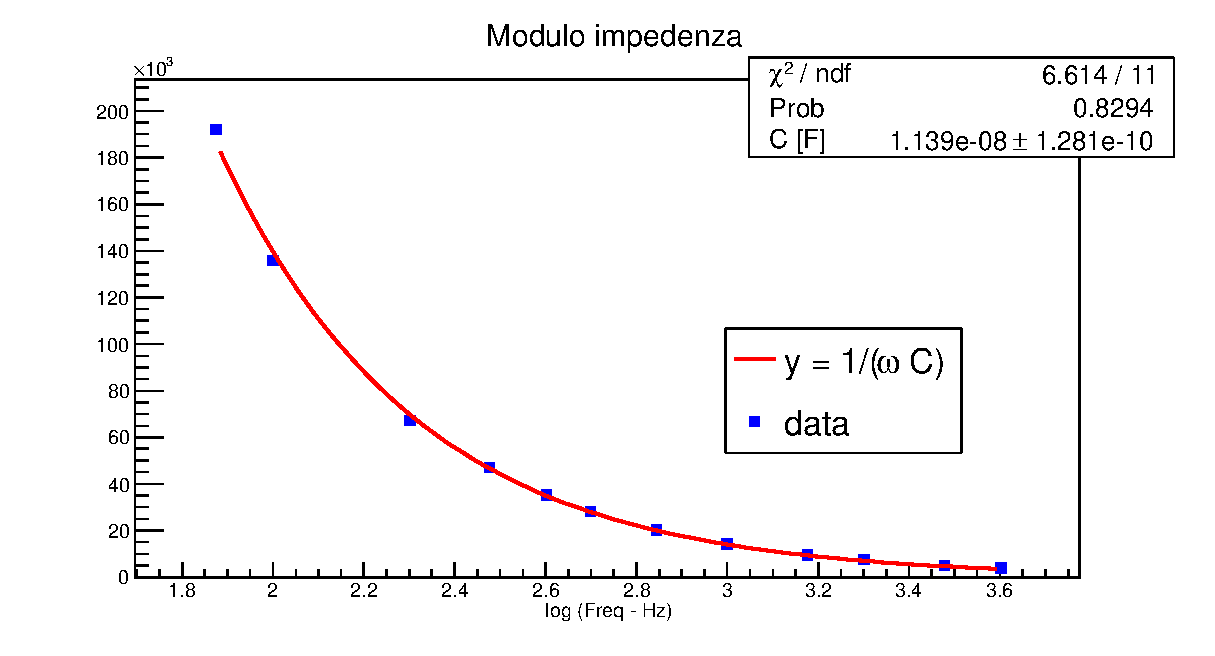
\includegraphics[scale=0.7]{Grafici/C3_P1_ModImp_cond1.eps}
\caption{
Circuito RC serie.
Ascisse [log( Freq. [Hz])].
Resistenza circuito 14870+50 [ohm]
Condensatore 11 [nF].
}
\label{fig:C3_P1_ModImp_cond1}
\end{figure}

\begin{figure}[H]
\centering
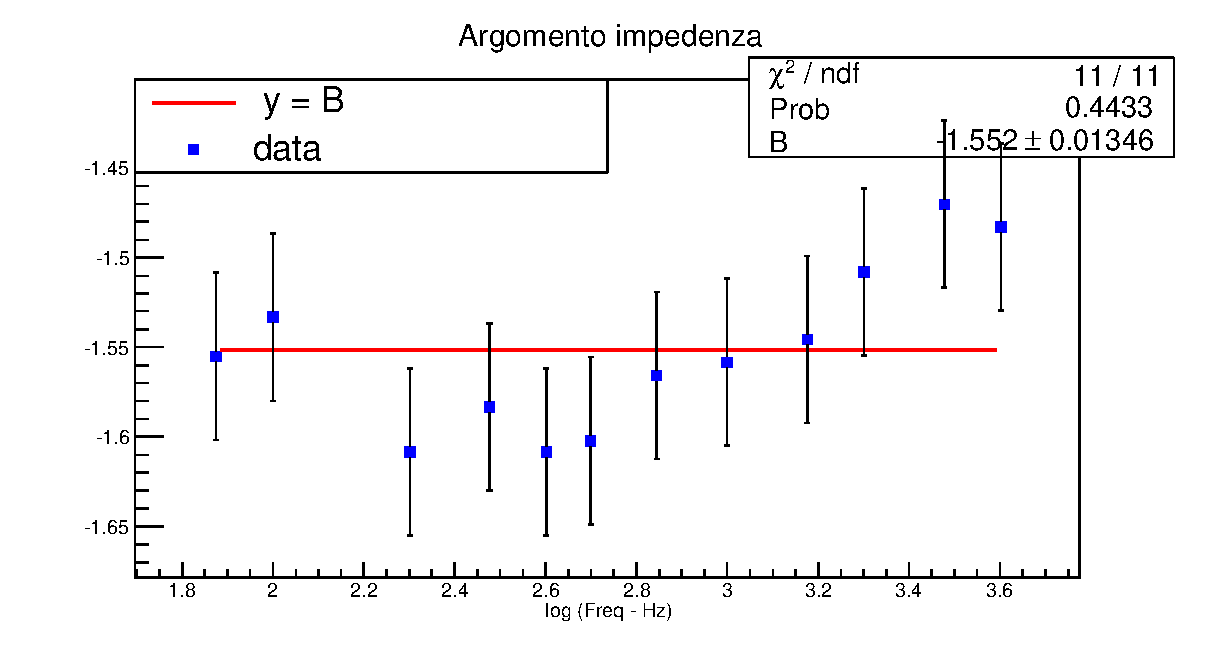
\includegraphics[scale=0.7]{Grafici/C3_P1_ArgImp_cond1.eps}
\caption{
Circuito RC serie.
Ascisse [log( Freq. [Hz])].
Resistenza circuito 14870+50 [ohm]
Condensatore 11 [nF].
}
\label{fig:C3_P1_ArgImp_cond1}
\end{figure}

\begin{figure}[H]
\centering
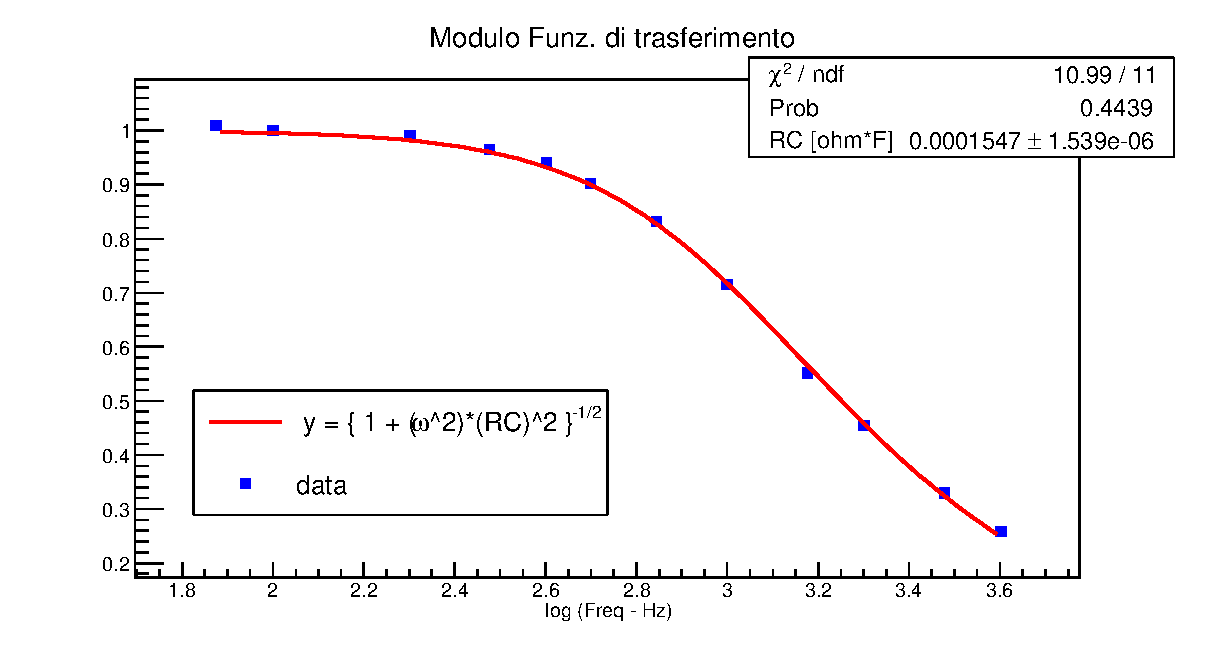
\includegraphics[scale=0.7]{Grafici/C3_P1_ModFdT_cond1.eps}
\caption{
Circuito RC serie.
Ascisse [log( Freq. [Hz])].
Resistenza circuito 14870+50 [ohm]
Condensatore 11 [nF].
}
\label{fig:C3_P1_ModFdT_cond1}
\end{figure}

\begin{figure}[H]
\centering
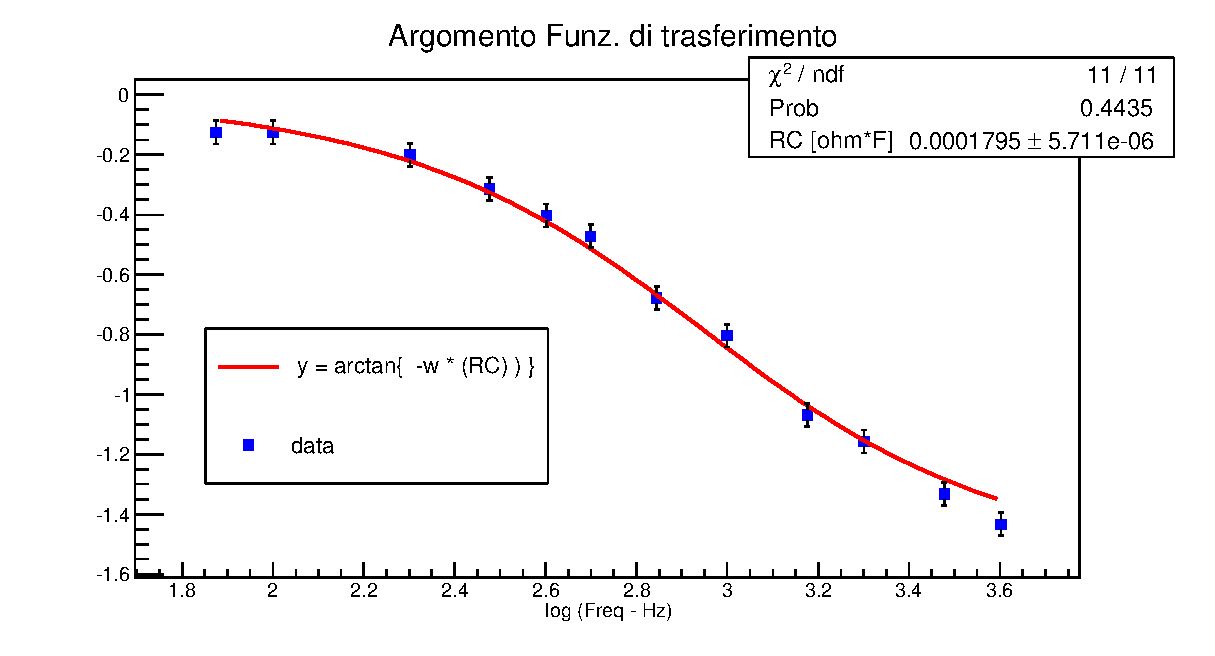
\includegraphics[scale=0.7]{Grafici/C3_P1_ArgFdT_cond1.eps}
\caption{
Circuito RC serie.
Ascisse [log( Freq. [Hz])].
Resistenza circuito 14870+50 [ohm]
Condensatore 11 [nF].
}
\label{fig:C3_P1_ArgFdT_cond1}
\end{figure}


%%%%%%%%%%%%%%%%%%%%%%%%%%%%%%%%%%%%%%%%%%%%%%
\begin{table}[H]
\begin{center}
\begin{tabular}{|r|r|r|r|r|r|r|r|}
\hline
\multicolumn{1}{|l|}{Freq} & \multicolumn{1}{l|}{Va} & \multicolumn{1}{l|}{Vb} & \multicolumn{1}{l|}{Vb-a} & \multicolumn{1}{l|}{-Fase (CH2)} & \multicolumn{1}{l|}{err-(CH2)} & \multicolumn{1}{l|}{-Fase (CH1)} & \multicolumn{1}{l|}{err-(CH1)} \\ \hline
\multicolumn{1}{|l|}{Hz} & \multicolumn{1}{l|}{V} & \multicolumn{1}{l|}{V} & \multicolumn{1}{l|}{V} & \multicolumn{1}{l|}{$\mu$s} & \multicolumn{1}{l|}{$\mu$s} & \multicolumn{1}{l|}{$\mu$s} & \multicolumn{1}{l|}{$\mu$s} \\ \hline
\multicolumn{1}{|c|}{$\pm$ 1} & \multicolumn{1}{c|}{$\pm$ 0.08} & \multicolumn{1}{c|}{$\pm$ 0.08} & \multicolumn{1}{c|}{$\pm$ 0.16} & \multicolumn{1}{l|}{} & \multicolumn{1}{c|}{$\pm$ } & \multicolumn{1}{l|}{} & \multicolumn{1}{c|}{$\pm$ } \\ \hline
75 & 10.2 & 0.80 & 10.3 & 3300 & 200 & 6400 & 200 \\ \hline
100 & 10.2 & 1.12 & 10.2 & 2,440 & 80 & 4800 & 80 \\ \hline
200 & 10.2 & 2.24 & 10.1 & 1,280 & 40 & 2340 & 40 \\ \hline
300 & 10.2 & 3.12 & 9.84 & 840 & 40 & 1500 & 40 \\ \hline
400 & 10.2 & 4.08 & 9.60 & 640 & 20 & 1090 & 20 \\ \hline
500 & 10.2 & 4.88 & 9.20 & 510 & 20 & 850 & 20 \\ \hline
700 & 10.1 & 6.16 & 8.40 & 356 & 8 & 560 & 8 \\ \hline
1000 & 10.3 & 7.68 & 7.36 & 248 & 8 & 372 & 8 \\ \hline
1500 & 10.3 & 8.88 & 5.68 & 164 & 4 & 220 & 4 \\ \hline
2000 & 10.2 & 9.36 & 4.64 & 120 & 4 & 158 & 4 \\ \hline
3000 & 10.2 & 9.92 & 3.36 & 78 & 2 & 96 & 2 \\ \hline
4000 & 10.2 & 10.0 & 2.64 & 59 & 2 & 68 & 2 \\ \hline
\end{tabular}
\end{center}
\caption{Condensatore 11 [nF]. Resistore 14.870 [ohm]}
\label{C3_P1_cond1}
\end{table}










%%%%%%%%%%%%%%%%%%%%%%%%%%%%%%%%%%%%%%%%%%%%%%
%%%%%%%%%%%%%%%%%%%%%%%%%%%%%%%%%%%%%%%%%%%%%%
\break
\subsubsection*{Condensatore 46 nF: grafici e dati}

%%%%%%%%%%%%%%%%%%%%%%%%%%%%%%%%%%%%%%%%%%%%%%
\begin{figure}[H]
\centering
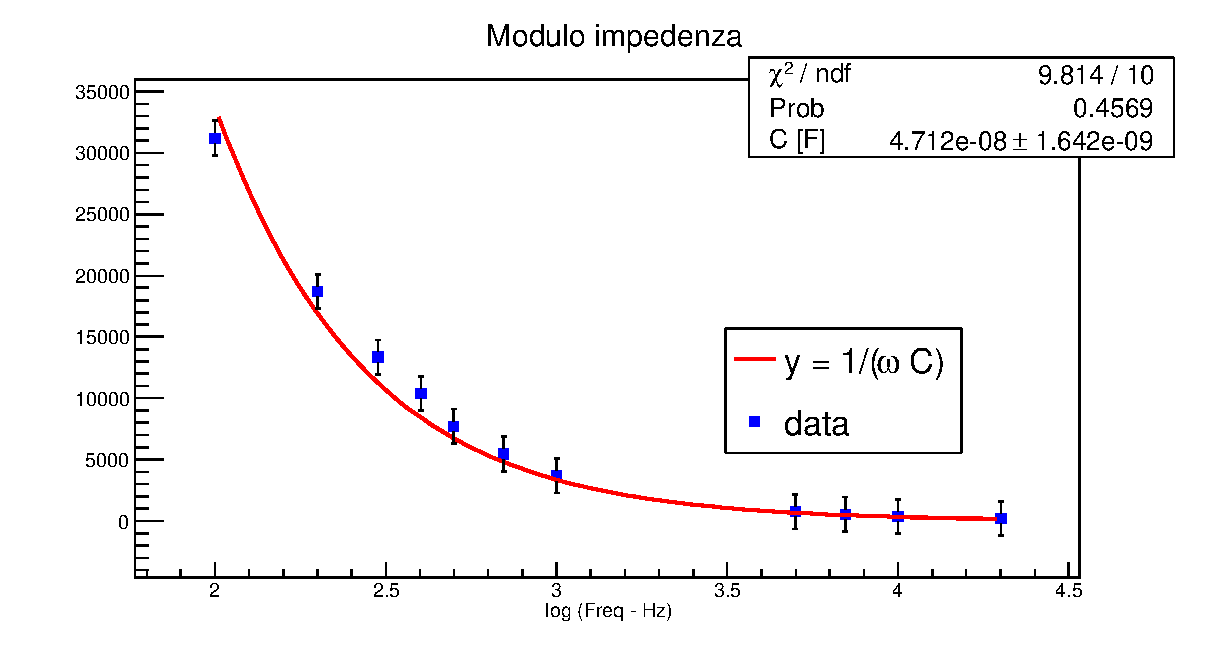
\includegraphics[scale=0.7]{Grafici/C3_P1_ModImp_cond2.eps}
\caption{
Circuito RC serie.
Ascisse [log( Freq. [Hz])].
Resistenza circuito 677+50 [ohm]
Condensatore 46 [nF].
}
\label{fig:C3_P1_ModImp_cond2}
\end{figure}

\begin{figure}[H]
\centering
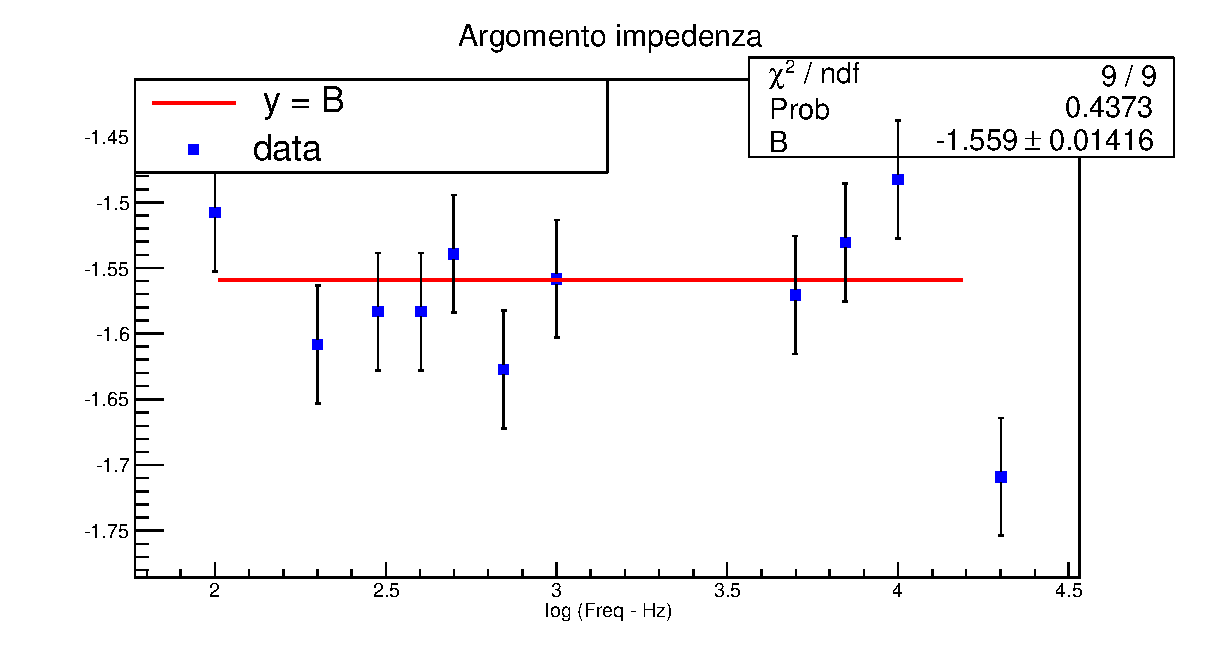
\includegraphics[scale=0.7]{Grafici/C3_P1_ArgImp_cond2.eps}
\caption{
Circuito RC serie.
Ascisse [log( Freq. [Hz])].
Resistenza circuito 677+50 [ohm]
Condensatore 46 [nF].
}
\label{fig:C3_P1_ArgImp_cond2}
\end{figure}

\begin{figure}[H]
\centering
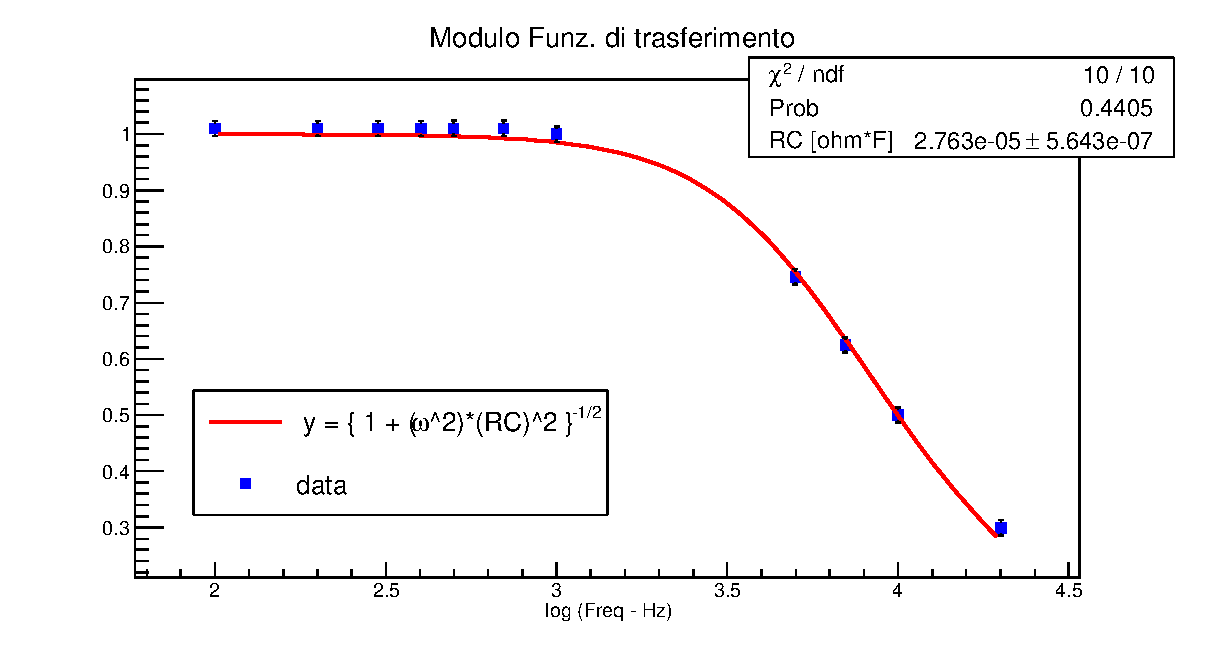
\includegraphics[scale=0.7]{Grafici/C3_P1_ModFdT_cond2.eps}
\caption{
Circuito RC serie.
Ascisse [log( Freq. [Hz])].
Resistenza circuito 677+50 [ohm]
Condensatore 46 [nF].
}
\label{fig:C3_P1_ModFdT_cond2}
\end{figure}

\begin{figure}[H]
\centering
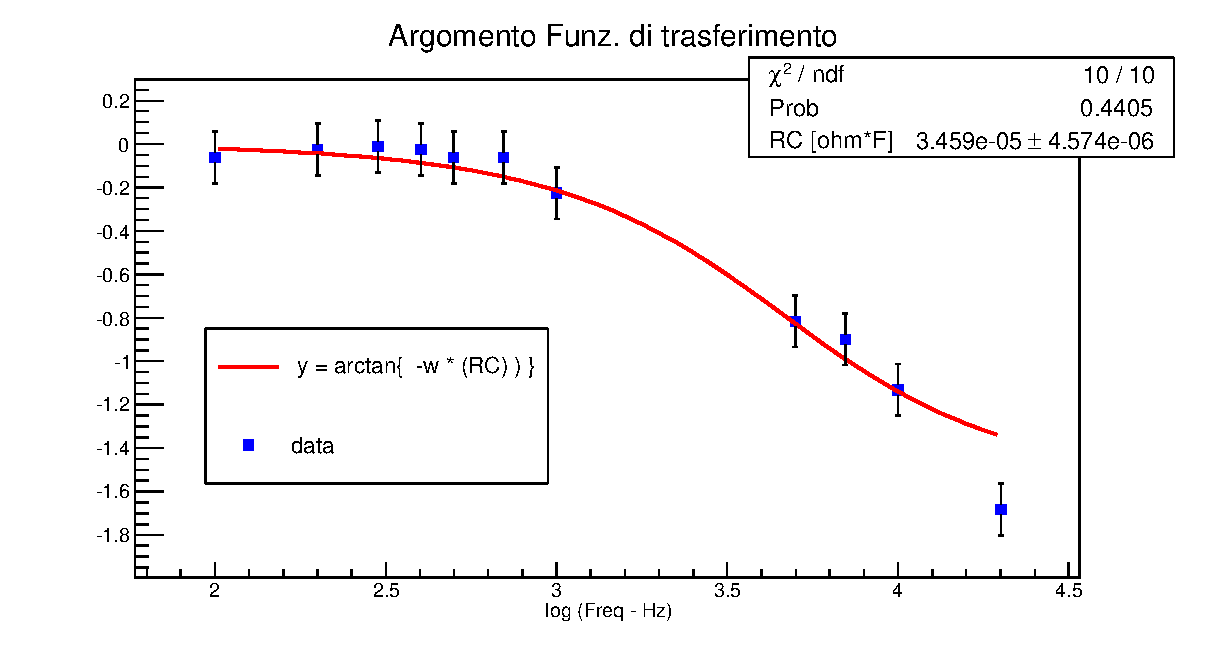
\includegraphics[scale=0.7]{Grafici/C3_P1_ArgFdT_cond2.eps}
\caption{
Circuito RC serie.
Ascisse [log( Freq. [Hz])].
Resistenza circuito 677+50 [ohm]
Condensatore 46 [nF].
}
\label{fig:C3_P1_ArgFdT_cond2}
\end{figure}


%%%%%%%%%%%%%%%%%%%%%%%%%%%%%%%%%%%%%%%%%%%%%%
\begin{table}[H]
\begin{center}
\begin{tabular}{|r|r|r|r|r|r|r|r|}
\hline
\multicolumn{1}{|l|}{Freq} & \multicolumn{1}{l|}{Va} & \multicolumn{1}{l|}{Vb} & \multicolumn{1}{l|}{Vb-a} & \multicolumn{1}{l|}{-Fase (CH2)} & \multicolumn{1}{l|}{err-(CH2)} & \multicolumn{1}{l|}{-Fase (CH1)} & \multicolumn{1}{l|}{err-(CH1)} \\ \hline
\multicolumn{1}{|l|}{Hz} & \multicolumn{1}{l|}{V} & \multicolumn{1}{l|}{V} & \multicolumn{1}{l|}{V} & \multicolumn{1}{l|}{$\mu$s} & \multicolumn{1}{l|}{$\mu$s} & \multicolumn{1}{l|}{$\mu$s} & \multicolumn{1}{l|}{$\mu$s} \\ \hline
\multicolumn{1}{|c|}{$\pm$ 1} & \multicolumn{1}{c|}{$\pm$ 0.08} & \multicolumn{1}{c|}{$\pm$ 0.08} & \multicolumn{1}{c|}{$\pm$ 0.16} & \multicolumn{1}{l|}{} & \multicolumn{1}{c|}{$\pm$ } & \multicolumn{1}{l|}{} & \multicolumn{1}{c|}{$\pm$ } \\ \hline
100 & 10.2 & 0.24 & 10.3 & 2400 & 200 & 4900 & 200 \\ \hline
200 & 10.2 & 0.40 & 10.3 & 1280 & 80 & 2480 & 80 \\ \hline
300 & 10.2 & 0.56 & 10.3 & 840 & 40 & 1660 & 40 \\ \hline
400 & 10.2 & 0.72 & 10.3 & 630 & 20 & 1240 & 20 \\ \hline
500 & 10.1 & 0.96 & 10.2 & 490 & 20 & 980 & 20 \\ \hline
700 & 10.1 & 1.36 & 10.2 & 370 & 20 & 700 & 20 \\ \hline
1000 & 10.2 & 2.00 & 10.2 & 248 & 8 & 464 & 8 \\ \hline
5000 & 9.76 & 6.88 & 7.28 & 50 & 2 & 74 & 2 \\ \hline
7000 & 9.60 & 7.92 & 6.00 & 34.8 & 0.8 & 51 & 0.8 \\ \hline
10000 & 9.44 & 8.64 & 4.72 & 23.6 & 0.8 & 32.0 & 0.8 \\ \hline
20000 & 9.36 & 9.20 & 2.80 & 13.6 & 0.4 & 11.6 & 0.4 \\ \hline
\end{tabular}
\end{center}
\caption{Condensatore 46 [nF]. Resistore 677 [ohm]}
\label{C3_P1_cond2}
\end{table}



















%%%%%%%%%%%%%%%%%%%%%%%%%%%%%%%%%%%%%%%%%%%%%%
%%%%%%%%%%%%%%%%%%%%%%%%%%%%%%%%%%%%%%%%%%%%%%
\break
\subsubsection{Induttori}

\paragraph{Modelli parametrici stimati}

A differenza dei condensatori, negli induttori si aggiunge la presenza di resistenza interna al componente stesso, l'impedenza è
$ Z = R_{p} + jwL $.


Dal modulo dell'impendenza si ricavano sia $ R_{p} $ che l'induttanza $L$, mentre dall'argomento risulta identificabile solo il loro rapporto
$ \theta = \frac{L}{R_{p}} $.

$$
|Z| = \sqrt{ R_{p}^2+ (Lw)^{2} }$$
$$
arg Z = \arctan( w\theta ), \quad \theta = \frac{L}{R_{p}}
$$



Per quanto riguarda la funzione di trasferimento, si tratta invece della resistenza totale del circuito $R_{t}$, che comprende quella del generatore e quella interna dell'induttore.

$$
|H| =   \frac{wL}{\sqrt{ R_{t}^{2} + (wL)^{2} } } 
$$
$$
arg H = \arctan( \frac{1}{w\gamma} ) \quad \gamma = \frac{L}{R_{t}}
$$

\paragraph{Dati} $ |Z| $ è il rapporto della differenza di potenziale $  V_{b-a} $ con la corrente misurata come $ V_{b} / R_{tot} $. In $ R_{tot} $ si tiene conto sia del resistore nel circuito, che della resistenza interna del generatore $50$ $\Omega$, nonchè della resistenza propria dell'induttore $R_{p} = 60$ $\Omega$, come misurata con multimetro palmare:
$ R_{t} = (677 + 50 + 60 )$ $\pm 1\%$.

\break
\paragraph{Risultati e commenti}

Per quanto riguarda il primo induttore, le stime di $L$ derivanti dal modulo dell'impedenza e da quello della funzione di trasferimento sono concordi sul valore di $0.1$ $H$, ma con un risultato più preciso di tre ordini di grandezza per la prima misura.

Per quanto riguarda la stima di $ R_{p} $, i risultati ottenuti non permettono di trarre conclusioni, a causa degli errori troppo alti.


\begin{table}[H]
\begin{center}
\begin{tabular}{|c|c|c|c|c|c|c|}
\hline

\multicolumn{2}{|c|}{Misura}  & Parametro   & U.ta & Stima & $\pm$ Errore & Chi2    \\ \hline

\multirow{ 3}{*}{Imp}
& \multirow{ 2}{*}{mod} & $R_{p}$ &  $[\Omega]$    
&  211 & $\pm$ 315 & \multirow{ 2}{*}{ 4 / 4 }     \\ 

&  & L  & $[H]$     
&   0.107 & $\pm$    0.001 &      \\

& arg & $ \tfrac{L}{R_{p}} $ & $[H / \Omega]$
& 0.00155 & $\pm$ 0.00014 &  4 / 4    \\ \hline


\multirow{ 2}{*}{FdT}
& \multirow{ 2}{*}{mod}
& $L$ & $ H $     
& 0.1  & $\pm$ 1.8     & \multirow{ 2}{*}{ 4 / 4 }  \\ 

& & $R_{t}$ & $[\Omega] $ 
& 724     & $\pm$ 11760 &      \\

& arg & $ \tfrac{L}{R_{t}} $ & $ H / \Omega $ 
& 0.0003  & $\pm$  0.0002 &      \\

\multicolumn{2}{|c|}{}  & $R_{t}$ & $[\Omega]$  
& 677 + 50 + 60  & $\pm$  10 &       \\ \hline

\end{tabular}

\label{C3_P1_fit_cond1}

\caption{
Fit output primo induttore.
}

\end{center}

\end{table}

Per quanto riguarda il secondo induttore, le stime dal modulo dell'impendeza forniscono risultati tra loro coerenti. Anche in questo caso, le misure derivanti dal modulo dell'impendenza sono molto più precise rispetto a quelle derivanti dal modulo della funzione di trasferimento. 
%
Il rapporto $ L / R_{p} $ derivante dall'argomento dell'impedenza si scosta leggermente dal rapporto delle stime derivante dal modulo. La causa di questo scostamento è da attribuirsi alla maggiore dispersione dei dati osservati rispetto al modello teorico stimato.\\ 
%
Per quanto riguarda le stime derivanti dalla funzione di trasferimento, anche per questo componente, l'incertezza sulle stime non permette di trarre conclusioni.\\
%
%
\begin{table}[H]
\begin{center}
\begin{tabular}{|c|c|c|c|c|c|c|}
\hline

\multicolumn{2}{|c|}{Misura}  & Parametro   & U.ta & Stima & $\pm$ Errore & Chi2     \\ \hline

\multirow{ 3}{*}{Imp}

& \multirow{ 2}{*}{mod} & $R_{p}$ &  $[\Omega]$    
&  72 & $\pm$    11 & \multirow{ 2}{*}{ 7 / 7 } \\ 

&  & L  & $[H]$     
&   0.0451 & $\pm$    0.0002 &  \\

& arg & $ \tfrac{L}{R_{p}} $ & $[H / \Omega]$
& $79\cdot 10^{-4}$ & $\pm$ $7.2\cdot 10^{-5}$ &  8 / 8 \\ \hline


\multirow{ 2}{*}{FdT}
& \multirow{ 2}{*}{mod} 

& $L$ & $ H $     
& 0.04  & $\pm$ 0.55     & \multirow{ 2}{*}{ 7 / 7 } \\

&
& $R_{t}$ & $ H $ 
& 814     & $\pm$ 9451 &  \\ 

& arg & $ \tfrac{L}{R_{p}} $ & $ H / \Omega $ 
& 0.0001  & $\pm$  0.0002 &   8 / 8  \\ \hline

\multicolumn{2}{|c|}{}  & $R_{t}$ & $[\Omega]$  
& 677 + 50 + 60  & $\pm$  10 &      \\ \hline

\end{tabular}

\label{C3_P1_fit_cond1}

\caption{
Fit output secondo induttore.
}

\end{center}

\end{table}
%
Fatte salve le osservazioni sulla generale scarsa precisione dei risultati ottenuti per i due induttori, si considerano come stime conclusive le stime dal modulo dell'impedenza, che presentano un errore di diversi ordini di grandezza inferiore a quelle provenienti dal modulo della funzione di trasferimento. Allo stesso risultato si perverrebbe considerando uno stimatore che combina le stime dai due esperimenti mediate per la rispettiva precisione relativa.
%
\begin{align*}
L_{1} & = 0.107   \pm 0.001 \;H \\
L_{2} & = 0.0451  \pm 0.0002 \;H
\end{align*}

\paragraph*{Note: Chi quadrato}
%
Vale quanto spiegato nel paragrafo \ref{Note Chi quadrato}



%%%%%%%%%%%%%%%%%%%%%%%%%%%%%%%%%%%%%%%%%%%%%%
%%%%%%%%%%%%%%%%%%%%%%%%%%%%%%%%%%%%%%%%%%%%%%
\break
\subsubsection*{Primo Induttore}

%%%%%%%%%%%%%%%%%%%%%%%%%%%%%%%%%%%%%%%%%%%%%%
\begin{figure}[H]
\centering
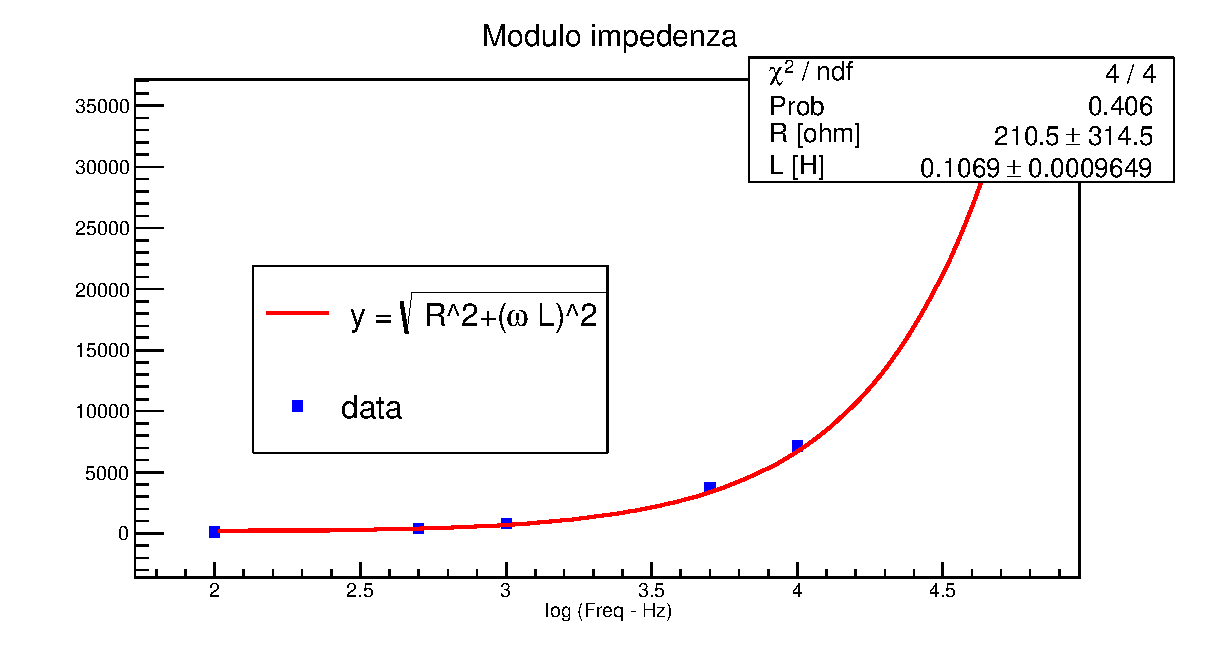
\includegraphics[scale=0.7]{Grafici/C3_P1_ModImp_ind1.eps}
\caption{
Circuito RL serie.
Ascisse [log( Freq. [Hz])].
Resistenza circuito 677+50 [ohm]
Primo induttore.
}
\label{fig:C3_P1_ModImp_ind1}
\end{figure}

\begin{figure}[H]
\centering
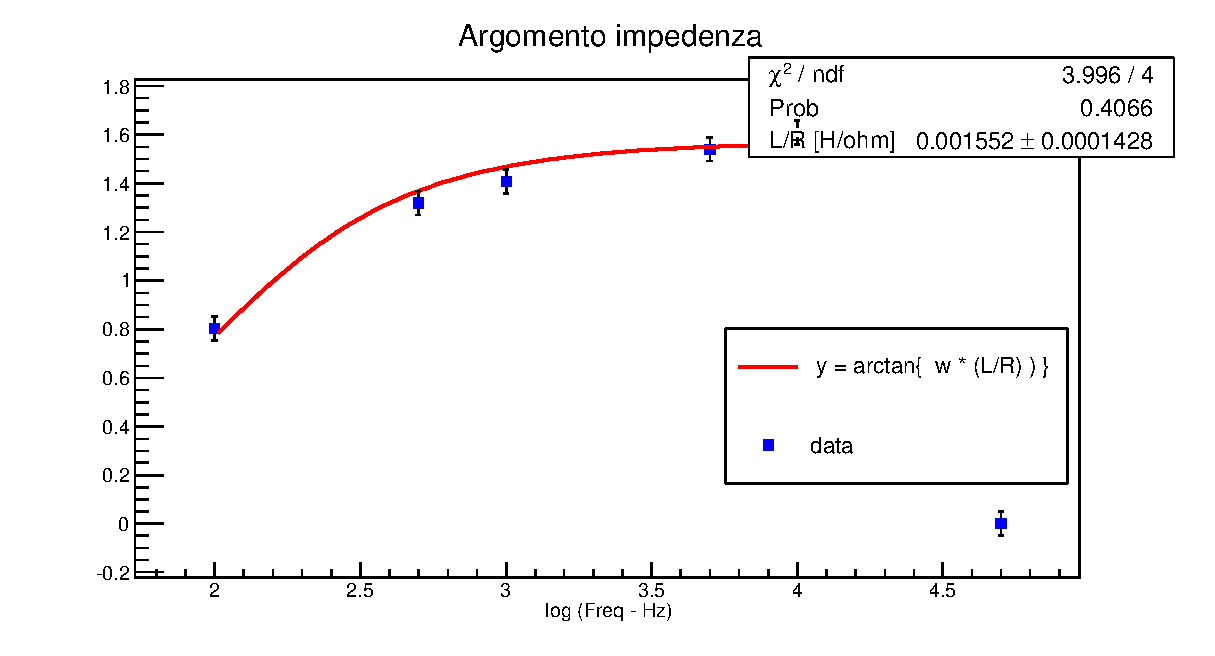
\includegraphics[scale=0.7]{Grafici/C3_P1_ArgImp_ind1.eps}
\caption{
Circuito RL serie.
Ascisse [log( Freq. [Hz])].
Resistenza circuito 677+50 [ohm]
Primo induttore.
}
\label{fig:C3_P1_ArgImp_ind1}
\end{figure}

\begin{figure}[H]
\centering
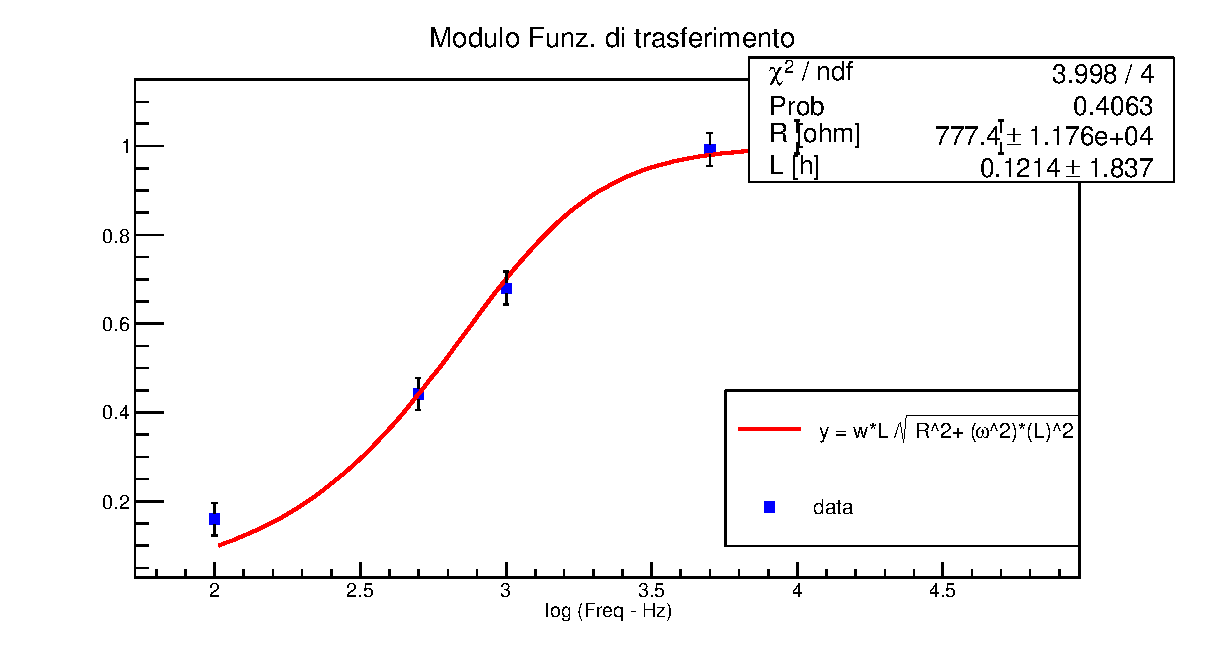
\includegraphics[scale=0.7]{Grafici/C3_P1_ModFdT_ind1.eps}
\caption{
Circuito RL serie.
Ascisse [log( Freq. [Hz])].
Resistenza circuito 677+50 [ohm]
Primo induttore.
}
\label{fig:C3_P1_ModFdT_ind1}
\end{figure}

\begin{figure}[H]
\centering
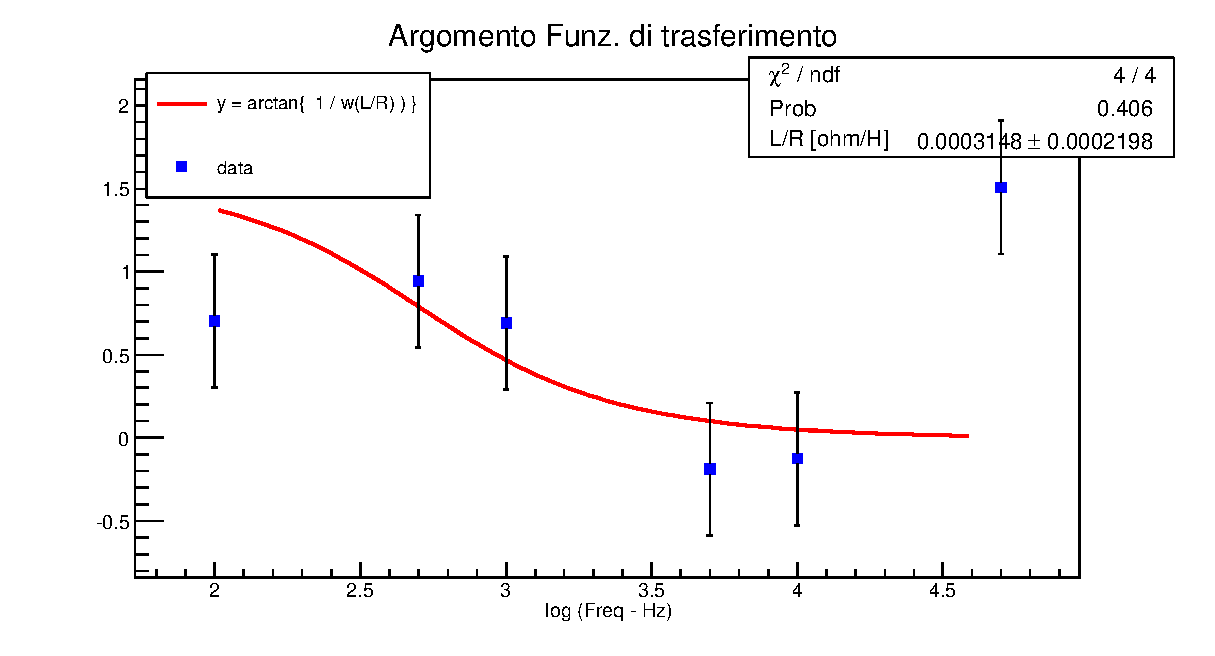
\includegraphics[scale=0.7]{Grafici/C3_P1_ArgFdT_ind1.eps}
\caption{
Circuito RL serie.
Ascisse [log( Freq. [Hz])].
Resistenza circuito 677+50 [ohm]
Primo induttore.
}
\label{fig:C3_P1_ArgFdT_ind1}
\end{figure}

\begin{table}[H]
\begin{center}
\begin{tabular}{|r|r|r|r|r|r|r|r|}
\hline
\multicolumn{1}{|l|}{Freq} & \multicolumn{1}{l|}{Va} & \multicolumn{1}{l|}{Vb} & \multicolumn{1}{l|}{Vb-a} & \multicolumn{1}{l|}{-Fase (CH2)} & \multicolumn{1}{l|}{err-(CH2)} & \multicolumn{1}{l|}{-Fase (CH1)} & \multicolumn{1}{l|}{err-(CH1)} \\ \hline
\multicolumn{1}{|l|}{Hz} & \multicolumn{1}{l|}{V} & \multicolumn{1}{l|}{V} & \multicolumn{1}{l|}{V} & \multicolumn{1}{l|}{$\mu$s} & \multicolumn{1}{l|}{$\mu$s} & \multicolumn{1}{l|}{$\mu$s} & \multicolumn{1}{l|}{$\mu$s} \\ \hline
\multicolumn{1}{|c|}{$\pm$ 1} & \multicolumn{1}{c|}{$\pm$ 0.08} & \multicolumn{1}{c|}{$\pm$ 0.08} & \multicolumn{1}{c|}{$\pm$ 0.2} & \multicolumn{1}{c|}{} & \multicolumn{1}{c|}{$\pm$ } & \multicolumn{1}{l|}{} & \multicolumn{1}{c|}{$\pm$ } \\ \hline
100 & 9.52 & 8.64 & 1.5 & 3720 & 80 & 3880 & 80 \\ \hline
500 & 9.60 & 7.92 & 4.2 & 580 & 40 & 700 & 40 \\ \hline
1000 & 9.76 & 6.56 & 6.6 & 276 & 8 & 390 & 8 \\ \hline
5000 & 10.0 & 2.08 & 9.9 & 51 & 2 & 106 & 2 \\ \hline
10000 & 10.00 & 1.12 & 10.2 & 24.4 & 0.8 & 52.0 & 0.8 \\ \hline
50000 & 10.00 & 0.24 & 10.2 & 10.0 & 0.2 & 5.2 & 0.2 \\ \hline
\end{tabular}
\end{center}
\caption{Primo induttore. Resistore 677 [ohm]}
\label{C3_P1_ind1}
\end{table}



%%%%%%%%%%%%%%%%%%%%%%%%%%%%%%%%%%%%%%%%%%%%%%
%%%%%%%%%%%%%%%%%%%%%%%%%%%%%%%%%%%%%%%%%%%%%%
\break
\subsubsection*{Secondo Induttore}

%%%%%%%%%%%%%%%%%%%%%%%%%%%%%%%%%%%%%%%%%%%%%%
\begin{figure}[H]
\centering
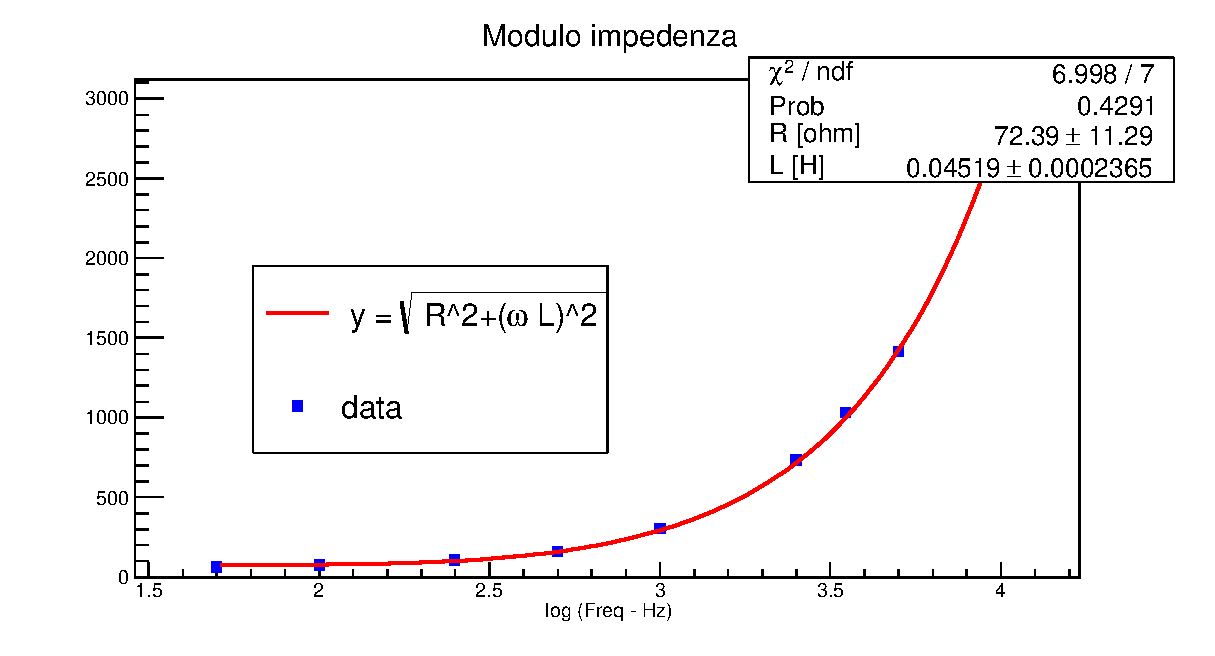
\includegraphics[scale=0.7]{Grafici/C3_P1_ModImp_ind2.eps}
\caption{
Circuito RL serie.
Ascisse [log( Freq. [Hz])].
Resistenza circuito 677+50 [ohm]
Secondo induttore.
}
\label{fig:C3_P1_ModImp_ind2}
\end{figure}

\begin{figure}[H]
\centering
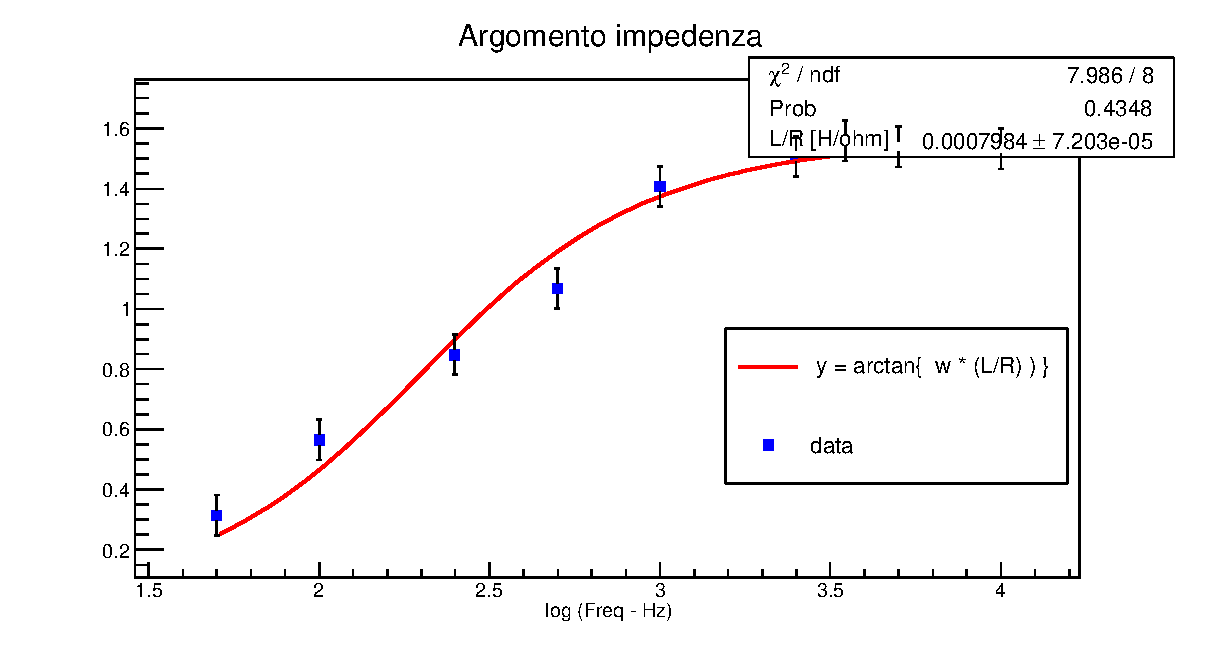
\includegraphics[scale=0.7]{Grafici/C3_P1_ArgImp_ind2.eps}
\caption{
Circuito RL serie.
Ascisse [log( Freq. [Hz])].
Resistenza circuito 677+50 [ohm]
Secondo induttore.
}
\label{fig:C3_P1_ArgImp_ind2}
\end{figure}

\begin{figure}[H]
\centering
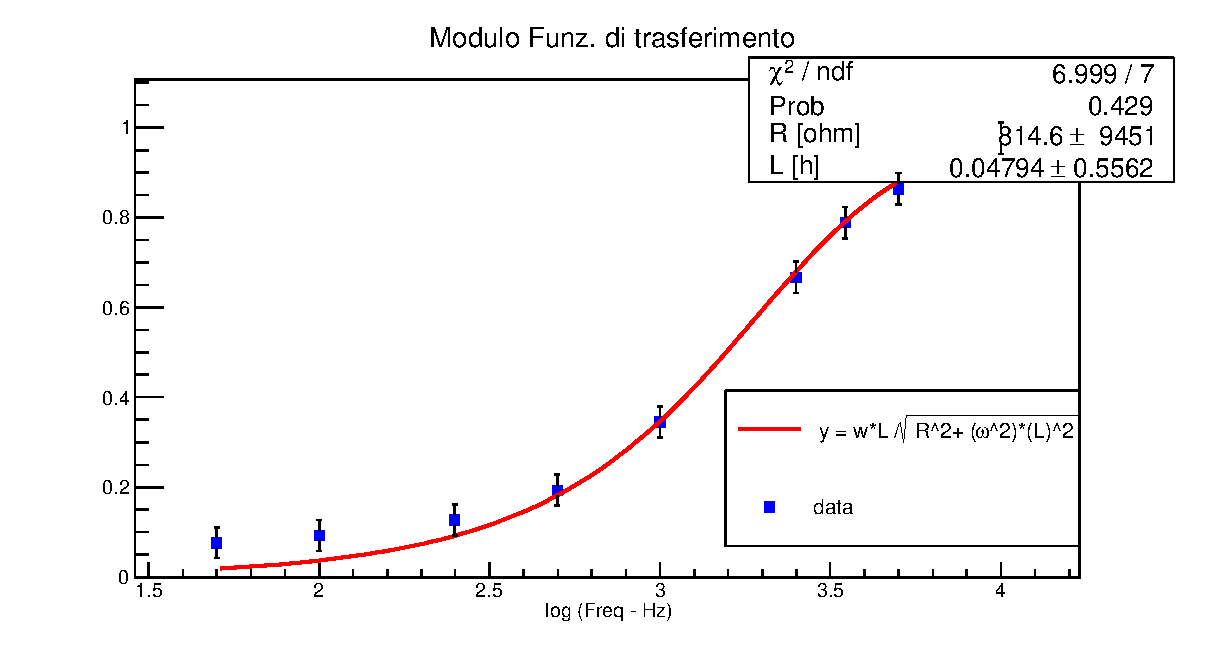
\includegraphics[scale=0.7]{Grafici/C3_P1_ModFdT_ind2.eps}
\caption{
Circuito RL serie.
Ascisse [log( Freq. [Hz])].
Resistenza circuito 677+50 [ohm]
Secondo induttore.
}
\label{fig:C3_P1_ModFdT_ind2}
\end{figure}

\begin{figure}[H]
\centering
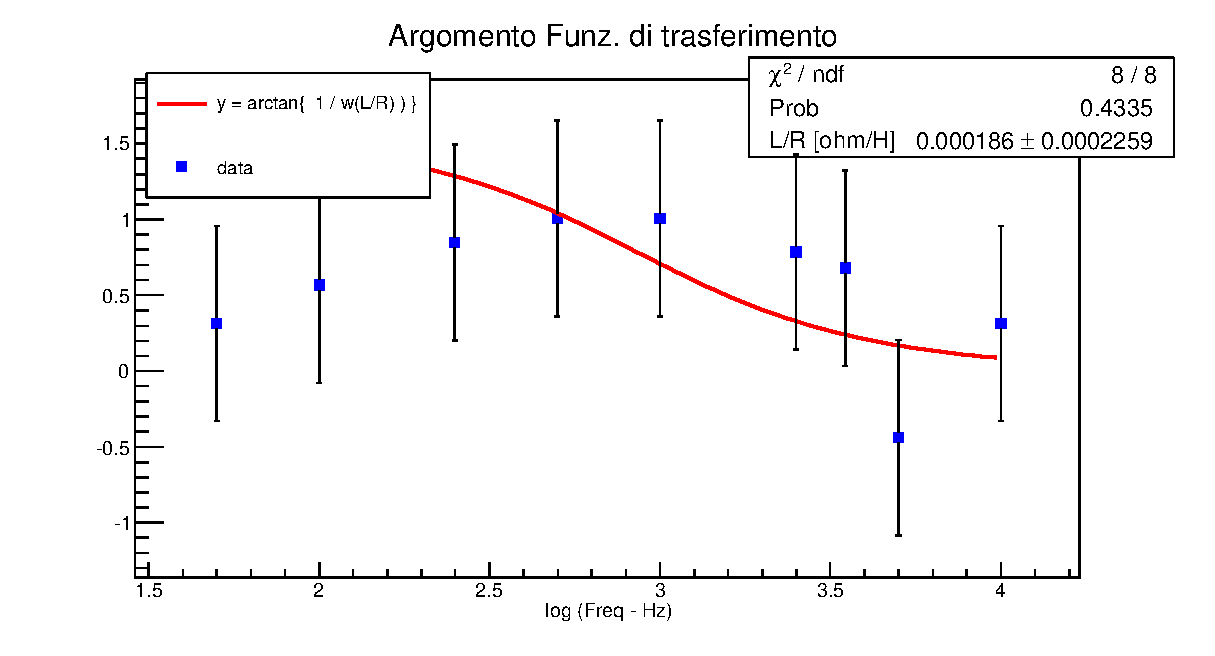
\includegraphics[scale=0.7]{Grafici/C3_P1_ArgFdT_ind2.eps}
\caption{
Circuito RL serie.
Ascisse [log( Freq. [Hz])].
Resistenza circuito 677+50 [ohm]
Secondo induttore.
}
\label{fig:C3_P1_ArgFdT_ind2}
\end{figure}

\begin{table}[H]
\begin{center}
\begin{tabular}{|r|r|r|r|r|r|r|r|}
\hline
\multicolumn{1}{|l|}{Freq} & \multicolumn{1}{l|}{Va} & \multicolumn{1}{l|}{Vb} & \multicolumn{1}{l|}{Vb-a} & \multicolumn{1}{l|}{-Fase (CH2)} & \multicolumn{1}{l|}{err-(CH2)} & \multicolumn{1}{l|}{-Fase (CH1)} & \multicolumn{1}{l|}{err-(CH1)} \\ \hline
\multicolumn{1}{|l|}{Hz} & \multicolumn{1}{l|}{V} & \multicolumn{1}{l|}{V} & \multicolumn{1}{l|}{V} & \multicolumn{1}{l|}{$\mu$s} & \multicolumn{1}{l|}{$\mu$s} & \multicolumn{1}{l|}{$\mu$s} & \multicolumn{1}{l|}{$\mu$s} \\ \hline
\multicolumn{1}{|c|}{$\pm$ 1} & \multicolumn{1}{c|}{$\pm$ 0.08} & \multicolumn{1}{c|}{$\pm$ 0.08} & \multicolumn{1}{c|}{$\pm$ 0.2} & \multicolumn{1}{l|}{} & \multicolumn{1}{c|}{$\pm$ } & \multicolumn{1}{l|}{} & \multicolumn{1}{c|}{$\pm$ } \\ \hline
50 & 9.44 & 9.04 & 0.72& 9000 & 400 & 9000 & 400 \\ \hline
100 & 9.52 & 9.04 & 0.9 & 4100 & 80 & 4100 & 80 \\ \hline
250 & 9.44 & 8.88 & 1.2 & 1460 & 40 & 1460 & 40 \\ \hline
500 & 9.52 & 8.88 & 1.8 & 660 & 40 & 680 & 40 \\ \hline
1000 & 9.52 & 8.48 & 3.3 & 276 & 8 & 340 & 8 \\ \hline
2500 & 9.84 & 7.04 & 6.6 & 104 & 4 & 150 & 4 \\ \hline
3500 & 9.84 & 5.92 & 7.8 & 72 & 4 & 112 & 4 \\ \hline
5000 & 10.0 & 4.80 & 8.6 & 51 & 2 & 114 & 2 \\ \hline
10000 & 10.0 & 2.72 & 9.8 & 25.6 & 0.8 & 45.0 & 0.8 \\ \hline
\end{tabular}
\end{center}
\caption{Secondo induttore. Resistore 677 [ohm]}
\label{C3_P1_ind2}
\end{table}

%Parte 2: Circuiti RC e RL in corrente impulsata
%\clearpage
\subsection{Parte 2: Circuito RC in corrente impulsata - carica e scarica}
\label{sec:C3_P2-1}

\subsubsection{Cenni Teorici}

Per la seconda legge di Kirchhoff, l'equazione del circuito RC è:
$$ V_{Resistore} + V_{Condensatore} = V_{generatore} $$
Si ha che $ V_{Resistore} = V_R = RI$ e $ V_{Condensatore} = V_C = \frac{Q}{C} $, dunque:
$$ R \frac{\mathrm d Q }{\mathrm d t} + \frac{Q}{C} = V_{generatore} $$
%

\subsubsection*{Carica (da $0$ a $V_0$)}

Si ha $V_{generatore} = V_0$, e la condizione iniziale $Q(t=0) = 0 $ (poichè un istante prima il generatore è spento).\\
Usando il metodo della separazione delle variabili, e ponendo $\tau = CR $, si trova la soluzione:
$$ Q(t) = CV_0(1-e^{-\frac{t}{\tau}})$$
Da cui:
\[
  \begin{cases}
    V_R(t) = I(t) R = \frac{\mathrm d Q(t) }{\mathrm d t} = V_0e^{-\frac{t}{\tau}}\\
    V_C(t) = V_0 - V_R(t) = V_0(1-e^{-\frac{t}{\tau}})\\
  \end{cases}
\]



\subsubsection*{Scarica (da $V_0$ a $0$)}

Si ha $V_{generatore} = 0$, e la condizione iniziale $Q(t=0) =CV_0 $ (poiché un istante prima il generatore eroga $V_0$).\\
Come prima, usando il metodo della separazione delle variabili, e ponendo $\tau = CR $, si trova la soluzione:
$$ Q(t) = CV_0 e^{-\frac{t}{\tau}}$$
Da cui:
\[
  \begin{cases}
    V_R(t) = I(t) R = \frac{\mathrm d Q(t) }{\mathrm d t} = -V_0e^{-\frac{t}{\tau}}\\
    V_C(t) = - V_R(t) = V_0-e^{-\frac{t}{\tau}}\\
  \end{cases}
\]

\newpage
\subsubsection{Analisi dati}
Seguono qui i dati fittati con le equazioni appena ricavate.\\
%
% Grafico RC
%
    \begin{figure}[H]
    \centering
    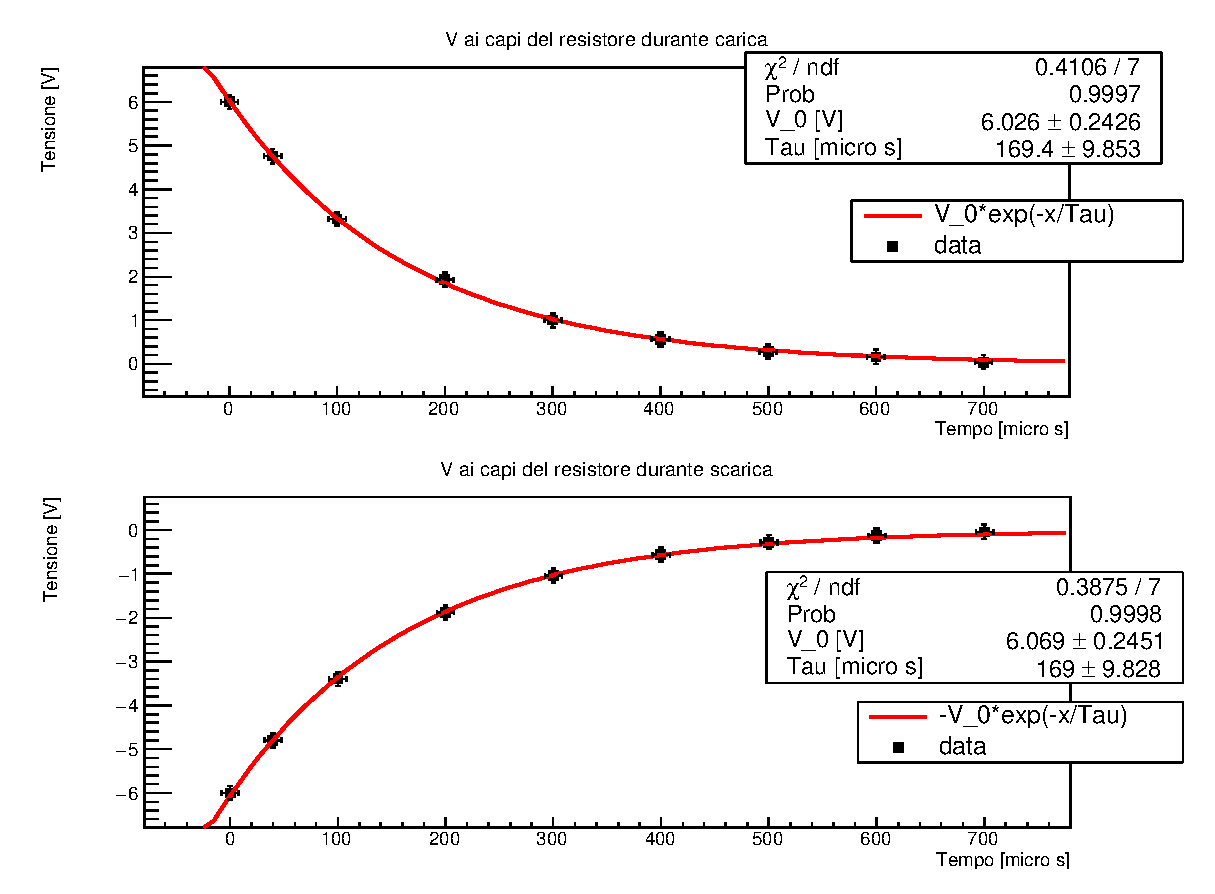
\includegraphics[scale=0.8]{Grafici/C3_P2_RC_impulsata_resistore.eps}
    %\caption{}
    \end{figure} 
%
    \begin{figure}[H]
    \centering
    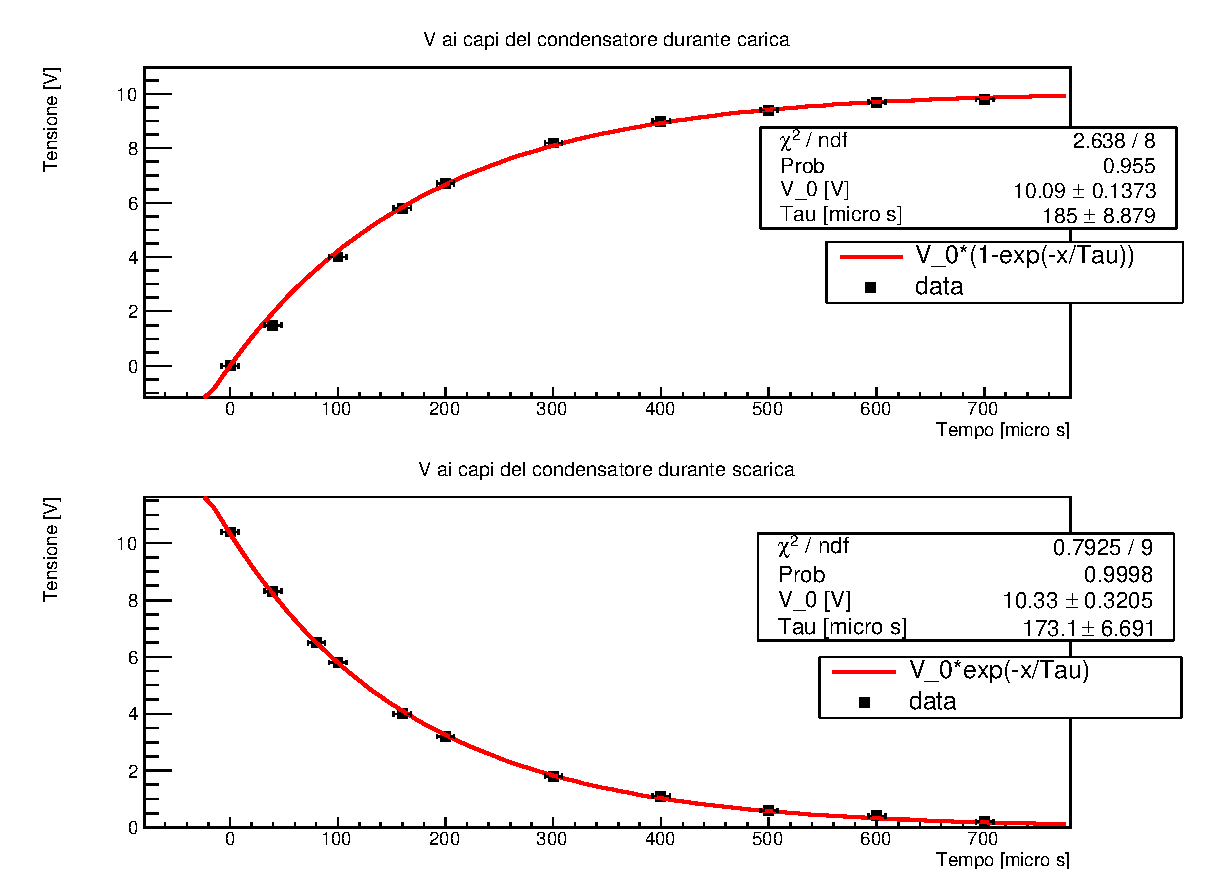
\includegraphics[scale=0.8]{Grafici/C3_P2_RC_impulsata_condensatore.eps}
    %\caption{}
    \end{figure} 
%
%
L'errore sulla tensione è stato stimato 0.16 V e quello per il tempo 8 µs (legati alla lettura dei valori con i cursori dell’oscilloscopio).\\
La resistenza usata è $14900 \pm 200$ Ohm (l'errore è stato calcolato come indicato sul manuale tecnico dello strumento).\\\\
%
%
Si ottiene il valore di $\tau$ con il suo errore calcolando la media pesata dei quattro valori ottenuti dai quattro fit.
%
Si ricava il valore della capacità $C$ e il suo errore, conoscendo la relazione $\tau = RC$ e utilizzando la formula di propagazione dell'errore.\\

Risultati ottenuti:
$$\tau = 174 \pm 4 \mu s $$
$$ C = 11.7 \pm 0.4  nF$$
%\clearpage
\subsection{Parte 2: Circuito RL in corrente impulsata - inversione del segno della tensione del generatore tra $-V_0$ e $+V_0$}

\subsubsection{Cenni Teorici}
%
Per la seconda legge di Kirchhoff, l'equazione del circuito RL è:
$$ V_{Resistore} + V_{Induttore} = V_{generatore} $$
Si ha che $ V_{Resistore} = V_R = RI$ e $ V_{Induttore} = V_L = L \frac{\mathrm d I }{\mathrm d t} $, dunque:
$$ RI + L \frac{\mathrm d I }{\mathrm d t} = V_{generatore} $$
%
\subsubsection*{Passaggio da $-V_0$ a $+V_0$}
Si ha $V_{generatore} = V_0$, e la condizione iniziale $I(t=0) = -\frac{V_0}{R} $ (poiché un istante prima il generatore eroga $-V_0$).\\
Usando il metodo della separazione delle variabili, e ponendo $\tau = \frac{L}{R} $, si trova la soluzione:
$$ I(t) = \frac{V_0}{R}(1-2e^{-\frac{t}{\tau}})$$
Da cui:
\[
  \begin{cases}
    V_R(t) = I(t) R = V_0(1-2e^{-\frac{t}{\tau}})\\
    V_L(t) = V_0 - V_R(t) = 2 V_0 e^{-\frac{t}{\tau}}\\
  \end{cases}
\]


\subsubsection*{Passaggio da $+V_0$ a $-V_0$}
Si ha $V_{generatore} = -V_0$, e la condizione iniziale $I(t=0) = \frac{V_0}{R} $ (poiché un istante prima il generatore eroga $+V_0$).\\
Come prima, usando il metodo della separazione delle variabili, e ponendo $\tau = \frac{L}{R} $, si trova la soluzione:
$$ I(t) = -\frac{V_0}{R}(1-2e^{-\frac{t}{\tau}})$$
Da cui:
\[
  \begin{cases}
    V_R(t) = I(t) R = -V_0(1-2e^{-\frac{t}{\tau}})\\
    V_L(t) = V_0 - V_R(t) = -2 V_0 e^{-\frac{t}{\tau}}\\
  \end{cases}
\]

\newpage
\subsubsection{Analisi dati}
Seguono qui i dati fittati con le equazioni appena ricavate.\\
%
% Grafico RL
%
    \begin{figure}[H]
    \centering
    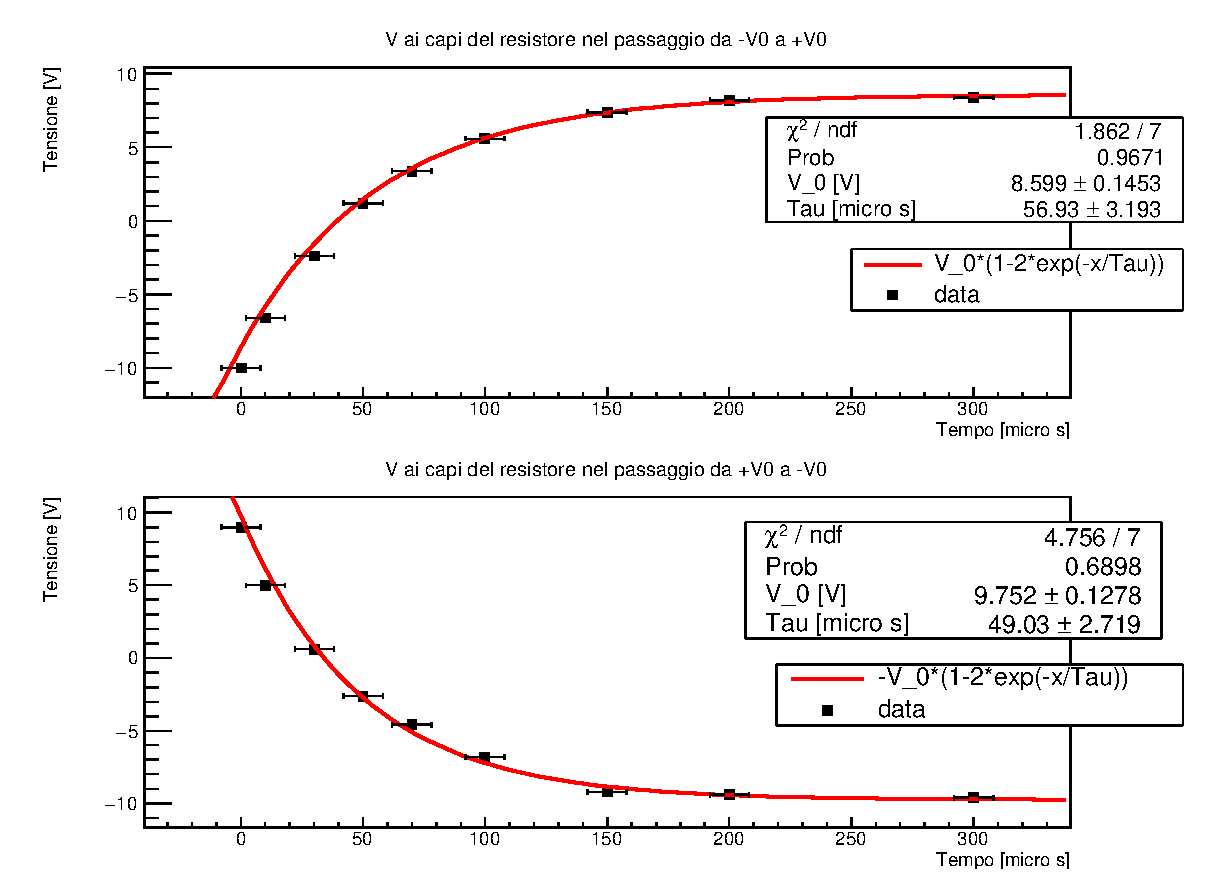
\includegraphics[scale=0.8]{Grafici/C3_P2_RL_impulsata_resistore.eps}
    %\caption{}
    \end{figure} 
%
    \begin{figure}[H]
    \centering
    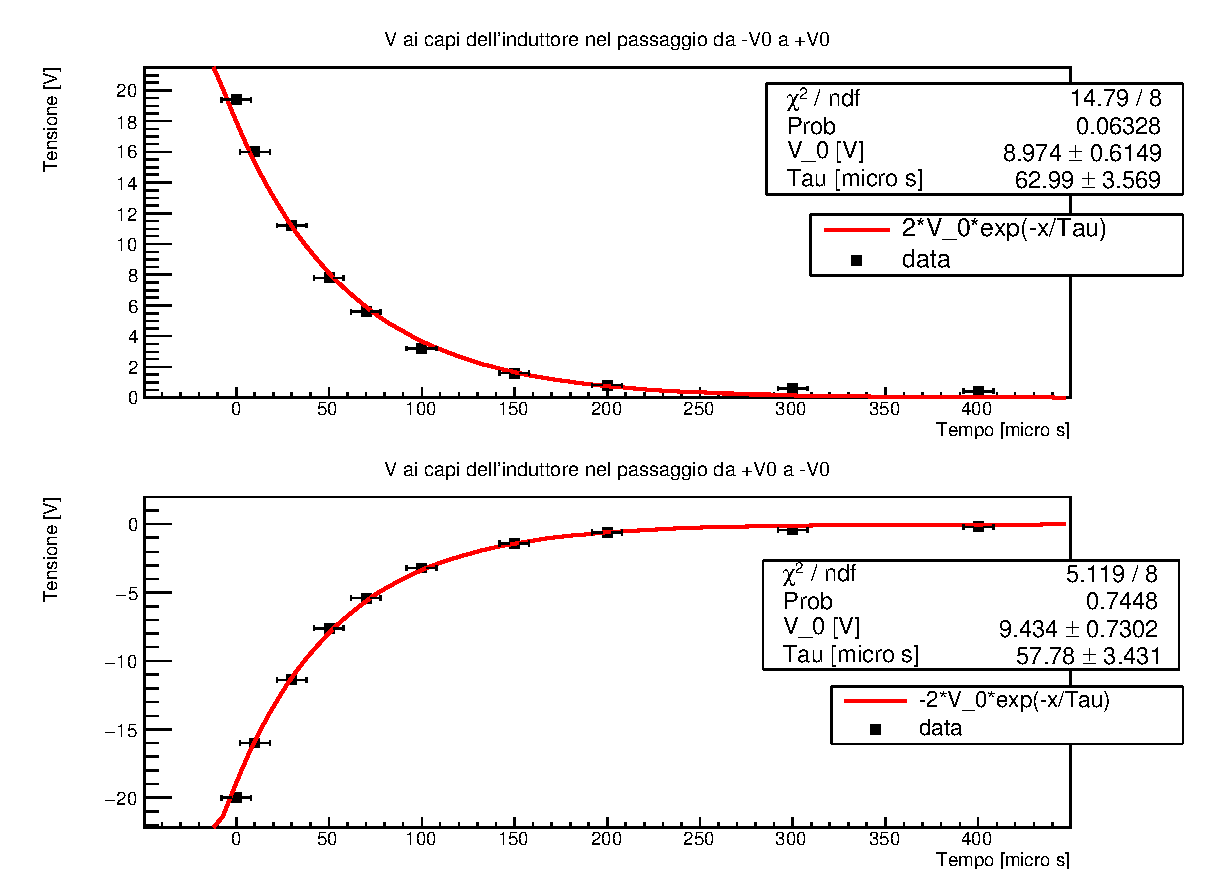
\includegraphics[scale=0.8]{Grafici/C3_P2_RL_impulsata_induttore.eps}
    %\caption{}
    \end{figure} 
%
%
La resistenza usata è $677 \pm 7$ Ohm (l'errore è stato calcolato come indicato sul manuale tecnico dello strumento).\\\\
%
%
Si ottiene il valore di $\tau$ con il suo errore calcolando la media pesata dei quattro valori ottenuti dai quattro fit (vedi fine paragrafo)
%
Si ricava il valore dell'induttanza $L$ e il suo errore, conoscendo la relazione $\tau = \frac{L}{R}$ e utilizzando la formula di propagazione dell'errore.\\

Risultati ottenuti:
$$\tau = 56 \pm 2 \mu s $$
$$ L = 0.038 \pm 0.001  H$$


%\subsection{Conclusioni}
\label{sec:C3_final}

\paragraph{Onda quadra}{ Nella pratica risulta impossibile realizzare un'onda perfettamente quadra poichè quando la tensione viene variata bruscamente il circuito ha dei tempi di risposta non istantanei. Se questo transiente dura $\delta t$, non nullo, mentre la parte a potenziale costante dura $\Delta t$, si ha che all'aumentare della frequenza  $\Delta t$ diminuisce. L'attesa è che $\delta t$ sia molto più influente ad alte frequenze poichè è maggiore il rapporto $\delta t/\Delta t$. Questo fenomeno non risulta evidente dai dati sperimentali.}
%
%
%
\paragraph{Metodo alternativo per la stima del tempo caratteristico}{Si osserva che all'aumentare della frequenza l'ampiezza massima della tensione aumenta in maniera monotona fino a raggiungere un massimo. Detto $\tau$ il tempo caratteristico di carica del condensatore e $T = 1/\nu$ il periodo dell'oscillazione del generatore, noto che $Q=V/C$ si osserva che:
\begin{itemize}
    \item per $T$ molto minore di $n\tau$ il condensatore non riesce a raggiungere la carica completa, quindi la tensione risulta bassa.
    \item per $T$ circa dell'ordine di $n\tau$ l'ampiezza raggiunge un massimo poichè la carica avviene in maniera completa
    \item per $T$ molto maggiore di $n\tau$ l'ampiezza si satura e il profilo tende a un'onda quadra, per l'argomento del paragrafo precedente.
\end{itemize}
Detta $\nu^*$ la frequenza in corrispondenza al massimo di ampiezza e $T^*$ il relativo periodo, se si assume $T^*$  è circa pari a $n\tau$, allora, noto R, si può ricavare C da:
    $$\tau =  CR \Rightarrow C \approx T^*/nR $$ }
%
\paragraph{Confronto misure} In questo esperimento le misure su induttanze e capacità sono state condotte nel dominio della frequenza (parte 1, impedenza e funzione di trasferimento) e nel dominio del tempo (parte 2, tempi caratteristici di carica e scarica). \\
%
Un confronto diretto tra le due misure è possibile solo per la capacità da $11$ $nF$, dove si evidenzia un parziale accordo fra le due.\\
%
Dai dati riportati, non risulta chiaro se uno dei due metodi sia preferibile all'altro quanto a precisione, a causa della forte diversità degli errori relativi da componente a componente.\\
%
A questo proposito si osserva che, nelle misure in corrente alternata, a causa della forte differenza tra errori sperimentali ed effettiva varianza dei residui di regressione, gli errori delle variabili dipendenti sono stati ricalcolati in modo da normalizzare il chi quadrato,
%
\begin{align*}
\chi^{2} &= \sum_{i=1}^{n}\frac{ ( y_{i}^{o} - y_{i}^{s})^{2} }{\sigma_{i}^{2}}    \\
\sigma^{2}_{ric} & = \sum_{i=1}^{n}\frac{ ( y_{i}^{o} - y_{i}^{s})^{2} }{gdl} 
\end{align*}
%
Senza tale normalizzazione gli errori relativi delle misure in corrente alternata risulterebbero in media più alti di quelli riportati, ma perchè sovrastimati rispetto all'effettiva varianza dei residui.
%
\begin{table}[H]
\begin{center}
\begin{tabular}{|c|c|c|c|}
\hline

 
Q.tà & U.tà  & \multicolumn{2}{|c|}{Misure}  \\
\multicolumn{2}{|c|}{}  
& Corr. Alternata & Corr. Impulsata \\\hline

\multirow{2}{*}{$L_{1}$} 
& \multirow{6}{*}{$[H]$}
& 0.107        &   \\
&
& $\pm 0.9\%$  &   \\

\multirow{2}{*}{$L_{2}$}
& 
&  0.0451        &   \\
&
&  $\pm 4\%$  &   \\

\multirow{2}{*}{$L_{3}$} 
&
&         &  0.038 \\
&
&         & $\pm 2.6\%$   \\\hline


\multirow{2}{*}{$C_{1}$} 
&  \multirow{4}{*}{$[nF]$}
& 11.38       & 11.7  \\
& 
& $\pm 1\%$  &  $\pm 3.4\%$   \\

\multirow{2}{*}{$C_{2}$} 
&  
& 47  &   \\
&
& $\pm 4\%$  &   \\\hline

\hline
\end{tabular}
\end{center}

\caption{Confronto precisone stime di capacità e induttanza in corrente alternata e impulsata. Errori relativi percentuali sono riportati sotto le relative stime.}
\label{C3_finale}

\end{table}




%\newpage

%%%%%%%%%%%%%%%%%%%%%%%%%%%%%%%%%%%%%%%%%%%%%%%%%%%%    
%%% C4

\section{Circuiti 4}

\subsection{Parte 1: circuito RLC in corrente impulsata}

Obiettivo dell'esperienza è la misura delle costanti caratteristiche del circuito RLC attraverso la rilevazione della forma d'onda del segnale di tensione, in funzione del tempo, nei tre regimi di smorzamento.

La dinamica di carica e scarica del circuito, è realizzata impostando un segnale di onda quadra con una frequenza sufficientemente bassa, in funzione dei tempi caratteristici di carica e scarica del circuito.

La rilevazione del segnale avviene con un oscilloscopio le cui sonde sono posizionate ai capi della resistenza.

La dinamica del sistema è matematicamente identica a quella di un oscillatore armonico smorzato con forzante costante, e può perciò essere convenientemente espressa anche in termini dei parametri meccanici $w_0^2$, la forza di richiamo per unità di massa e spostamento e $\gamma$, il coefficiente di smorzamento.

\begin{align*}
V_0    = & L\dot{I} + RI + Q/C   \\
0      = & \ddot{Q} + 2\gamma \dot{Q} + \omega_0^2(Q-Q_0) \\
\end{align*}

La parametrizzazione meccanicistica è stata utilizzata in fase di stima dei modelli parametrici nei tre regimi di smorzamento. 

Le stime e gli errori sui parametri elettrici sono stati ricavati successivamente usando le relazioni inverse che li legano a quelli meccanici.





%%%%%%%%%%%%%%%%%%%%%%%%%%%%%%%%%%%%%%%%%%%%%%%%%%
%%%%%%%%%%%%%%%%%%%%%%%%%%%%%%%%%%%%%%%%%%%%%%%%%%
%%%%%%%%%%% SOTTO



\subsubsection{Regime sottosmorzato}

Indicando con 
$\omega = \sqrt{\omega_0^2 - \gamma^2}$, $\gamma < \omega_0$,

\begin{align*}
V(t) / V_{0} =&  A \; e^{-\gamma t} \; [ \gamma \cos\omega t + \omega \sin\omega t ] \\
A =& RC
\end{align*}

Inteso come modello parametrico in funzione dei tre parametri incogniti $w$, $\gamma$ e $A$. $V_0$ è misurabile direttamente dal primo canale dell'oscilloscopio. L'adattamento è stato eseguito con fit non lineare sui dati

\begin{table}[H]
\begin{center}
\begin{tabular}{|c|c|c|c|}
\hline
Tempo & Ddp & Tempo & Ddp \\ \hline
$\mu s$ & $mV$ & $\mu s$ & $mV$ \\ \hline
$\pm 8$ & $\pm 16$ & $\pm 8$ & $\pm 16$ \\ \hline
0 & 0 & 412 & 352 \\ \hline
40 & 480 & 444 & 416 \\ \hline
84 & 728 & 476 & 352 \\ \hline
120 & 600 & 504 & 200 \\ \hline
160 & 224 & 532 & 0 \\ \hline
180 & 0 & 620 & -320 \\ \hline
200 & -200 & 716 & 0 \\ \hline
220 & -400 & 796 & 240 \\ \hline
264 & -560 & 972 & -184 \\ \hline
300 & -432 & 1150 & 144 \\ \hline
340 & -144 & 1330 & -104 \\ \hline
356 & 0 & 1500 & 88 \\ \hline
380 & 176 &  &  \\ \hline
\end{tabular}
\end{center}
\caption{ Sottosmorzato.
Resistenza 100 (+50+50)  [$\Omega$].
Capacità  46    [$nF$].
Induttore 0.065 [$H$].
}
\label{tab:C4_P1_sotto}
\end{table}

\begin{figure}[H]
\centering
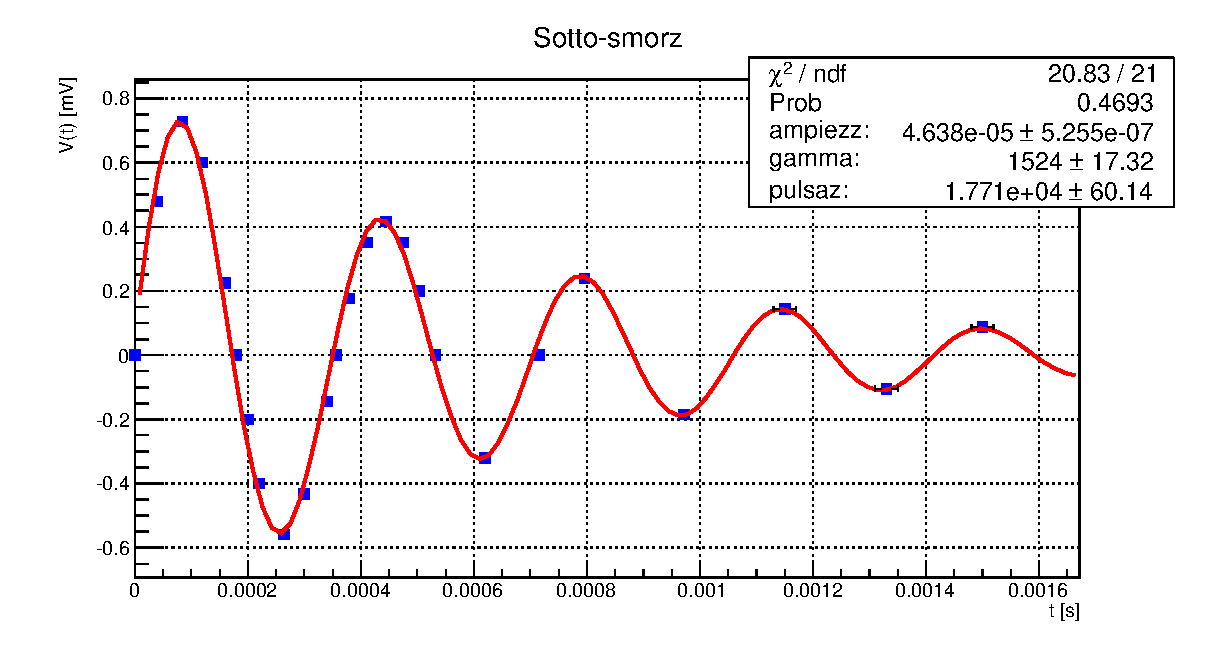
\includegraphics[scale=0.75]{Grafici/C4_P1_Sotto-smorz.eps}
\caption{
Circuito RLC serie. Regime sottosmorzato.
}
\label{fig:C4_P1_sotto}
\end{figure}

Nel regime sottosmorzato non è possibile ottenere una stima puntuale dei parametri $R$, $C$ e $L$ perchè lo jacobiano di trasformazione tra parametri elettrici e meccanici ha determinante nullo.

\begin{align*}
    A / V_0 = & RC   \\
    2\gamma    = & R/L   \\
    w_0^{-2} = (w^2+\gamma^2)^{-1}    = & RL
\end{align*}

Le alternative sono: (a) ottenere una misura diretta di $R_{tot}$ misurando la resistenza delle singole componenti con multimetro palmare. Oppure (b) combinare queste misure con altre ottenute negli altri regimi.

Qui di seguito i risultati ottenuti seguendo il metodo (a):

\begin{table}[H]
\begin{center}
\begin{tabular}{|c|c|c|c|}
\hline

Parametro & Misura & Unità & stima \\ \hline

$R_{tot}$ & diretta & $\Omega$ & $200\pm1\%$ \\ 

$C$ & indiretta & $nF$ & $46.4\pm3\%$ \\ 

$L$ & indiretta & $H$ & $0.066\pm2\%$ \\ 

\hline
\end{tabular}
\end{center}
\caption{
Misure indirette dei parametri C e L.
Regime sottosmorzato.
}
\label{C4_P1_sotto_fit}
\end{table}




%%%%%%%%%%%%%%%%%%%%%%%%%%%%%%%%%%%%%%%%%%%%%%%%%%
%%%%%%%%%%%%%%%%%%%%%%%%%%%%%%%%%%%%%%%%%%%%%%%%%%
%%%%%%%%%%% CRITICO



\subsubsection{Regime di smorzamento critico}

Alla condizione che $\omega_0 = \gamma$, il modello teorico per la ddp è

\begin{align*}
V(t)/ V_{0} =& A \gamma^{2} t e^{-\gamma t}    \\
A = & RC
\end{align*}

Inteso come modello parametrico in funzione dei due parametri incogniti $\gamma$ e $A$. $V_0$ è misurabile direttamente dal primo canale dell'oscilloscopio. L'adattamento è stato eseguito con fit non lineare sui dati


\begin{table}[H]
\begin{center}
\begin{tabular}{|c|c|c|c|}
\hline
Tempo & Ddp & Tempo & Ddp \\ \hline
$\mu s$ & $mV$ & $\mu s$ & $mV$ \\ \hline
$\pm 4$ & $\pm 80$ & $\pm 4$ & $\pm 80$ \\ \hline
0 & 0 & 74 & 6920 \\ \hline
4 & 1320 & 84 & 6520 \\ \hline
8 & 2480 & 100 & 5880 \\ \hline
12 & 3400 & 124 & 4760 \\ \hline
18 & 4560 & 150 & 3640 \\ \hline
24 & 5480 & 185 & 2400 \\ \hline
34 & 6520 & 210 & 1720 \\ \hline
44 & 7040 & 234 & 1240 \\ \hline
51 & 7200 & 310 & 440 \\ \hline
54 & 7280 & 402 & 120 \\ \hline
64 & 7160 & \multicolumn{1}{l|}{} & \multicolumn{1}{l|}{} \\ \hline
\end{tabular}
\end{center}
\caption{Smorzamento critico.
Resistenza 2390 (+50+50)   [$\Omega$].
Capacità  46    [$nF$].
Induttore 0.065 [$H$].
}
\label{tab:C4_P1_critico}
\end{table}        

\begin{figure}
\centering
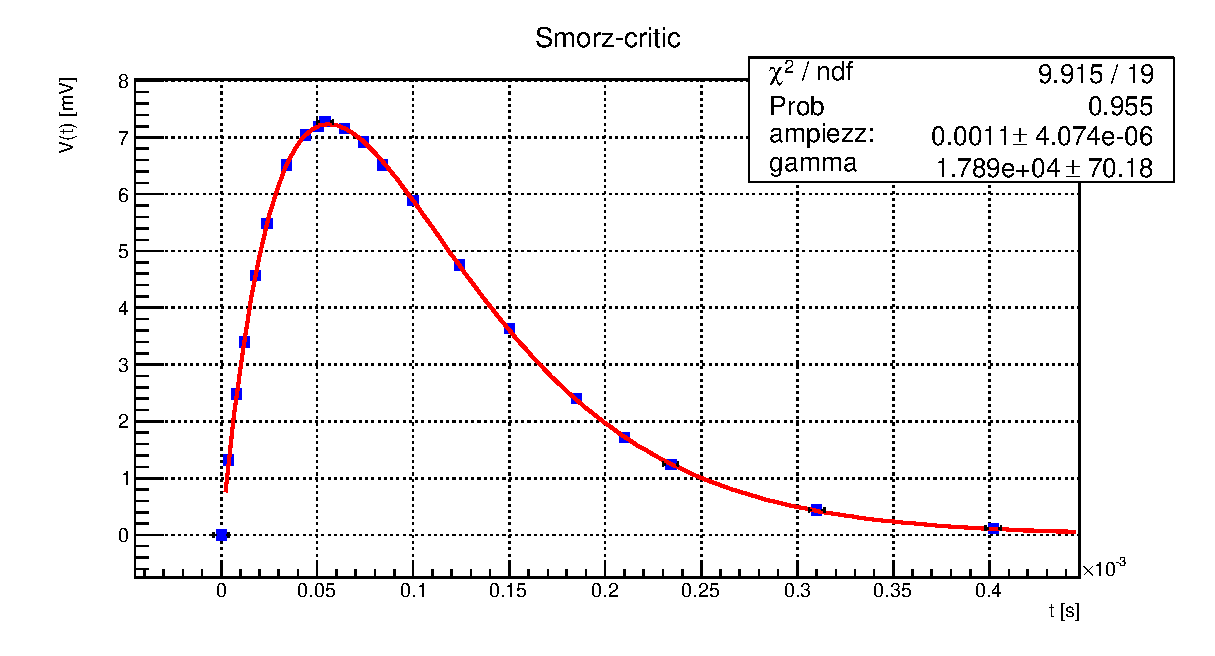
\includegraphics[scale=0.75]{Grafici/C4_P1_Smorz-critic.eps}
\caption{
Circuito RLC serie. Regime di smorzamento critico.
}
\label{fig:C4_P1_critico}
\end{figure}

Nel regime di smorzamento critico non è possibile ottenere una stima puntuale dei parametri $R$, $C$ e $L$ non disponeno di sufficienti equazioni per esprimere i parametri elettrici in funzione di quelli meccanici.

\begin{align*}
    A / V_0 = & RC   \\
    2\gamma    = & R/L   \\
\end{align*}

Le alternative sono: (a) ottenere una misura diretta di $R_{tot}$ misurando la resistenza delle singole componenti con multimetro palmare. Oppure (b) combinare queste misure con altre ottenute negli altri regimi (c) usare la condizione di smorzamento critico

\begin{align*}
    4L = & R^{2}C
\end{align*}

Qui di seguito i risultati ottenuti seguendo il metodo (a):

\begin{table}[H]
\begin{center}
\begin{tabular}{|c|c|c|c|}
\hline

Parametro & Misura & Unità & stima \\ \hline

$R_{tot}$ & diretta & $\Omega$ & $2500\pm1\%$ \\ 

$C$ & indiretta & $nF$ & $87.9\pm2.4\%$ \\ 

$L$ & indiretta & $H$ & $0.069\pm1.4\%$ \\ 

\hline
\end{tabular}
\end{center}
\caption{
Misure indirette dei parametri C e L.
Regime di smorzamento critico.
}
\label{C4_P1_critico_fit}
\end{table}





%%%%%%%%%%%%%%%%%%%%%%%%%%%%%%%%%%%%%%%%%%%%%%%%%%
%%%%%%%%%%%%%%%%%%%%%%%%%%%%%%%%%%%%%%%%%%%%%%%%%%
%%%%%%%%%%% SOVRA



\subsubsection{Regime sovrasmorzato}

Alla condizione che $\omega_0 < \gamma$, il modello teorico per la ddp è

\begin{align*}
V(t) / V_{0} =& A \frac{ \omega_0^2}{2\beta} \; [e^{-(\gamma - \beta)t} - e^{-(\gamma + \beta)t} ] \\
\beta^2 =& \gamma^2 - \omega_0^2 
\end{align*}

Con questa parametrizzazione l'algoritmo di minimizzazione del fit non lineare non converge. Si riparametrizza il modello

\begin{align*}
V(t) / V_{0} =&
Q_{0}  B ( e^{-\theta t} - e^{-\eta t} ) \\
B = & \frac{ (\frac{\eta-\theta}{2})^2 + (\frac{\eta+\theta}{2})^2 }
{\theta + \eta} \\
\theta = & \beta-\gamma \\
\eta   = & \beta+\gamma
\end{align*}

in funzione ora dei tre parametri incogniti $Q_0$, $\eta$ e $\theta$.

\begin{table}[H]
\begin{center}
\begin{tabular}{|c|c|c|c|}
\hline
Tempo & Ddp & Tempo & Ddp \\ \hline
$\mu s$ & $mV$ & $\mu s$ & $mV$ \\ \hline
$\pm 1\%$ & $\pm 80$ & $\pm 1\%$ & $\pm 80$ \\ \hline
0 & 0 & 115 & 8080 \\ \hline
2.6 & 2560 & 180 & 7040 \\ \hline
4.6 & 4640 & 226 & 6320 \\ \hline
9 & 7440 & 340 & 4880 \\ \hline
14.6 & 8960 & 440 & 3920 \\ \hline
28.4 & 9760 & 680 & 2240 \\ \hline
43 & 9520 & 880 & 1440 \\ \hline
65 & 9120 & 1120 & 880 \\ \hline
89 & 8640 & 1870 & 240 \\ \hline
\end{tabular}
\end{center}
\caption{Sovrasmorzato
Resistenza 10.000 (+50+50)   [$\Omega$].
Capacità  46    [$nF$].
Induttore 0.065 [$H$].
}
\label{tab:C4_P1_sovra}
\end{table}

\begin{figure}
\centering
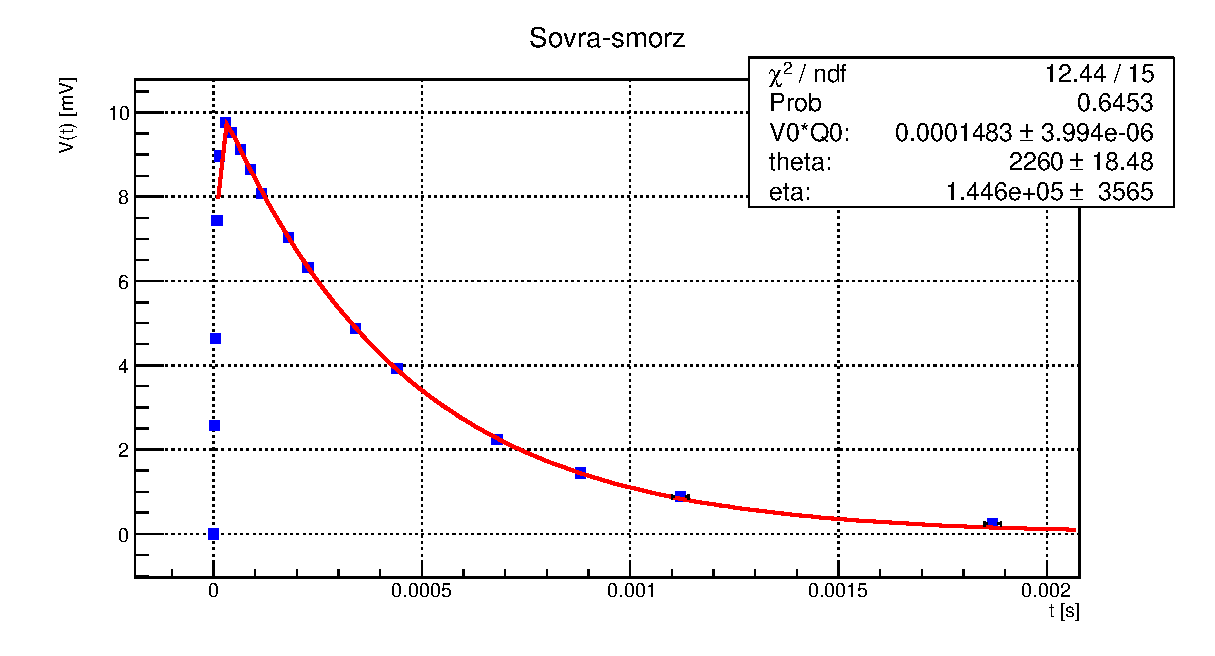
\includegraphics[scale=0.75]{Grafici/C4_P1_Sovra-smorz.eps}
\caption{
Circuito RLC serie. Regime sovrasmorzato.
}
\label{fig:C4_P1_sovra}
\end{figure}

Per ricavare ora i parametri elettrici si possono usare le seguenti relazioni

\begin{align}
&    CR = Q_0  \\
&    \frac{1}{CL} = w_0^2 = \frac{ (\frac{\eta-\theta}{2})^2 + (\frac{\eta+\theta}{2})^2 }
{\theta + \eta} \\
&    \frac{R}{L} = \eta-\theta
\end{align}

Usando una misura diretta di $R$, come fatto anche nei primi due regimi, si ricavano i seguenti risultati per $C$ e $L$ dalla prima e dalla terza relazione.

\begin{table}[H]
\begin{center}
\begin{tabular}{|c|c|c|c|}
\hline

Parametro & Misura & Unità & stima \\ \hline

$R_{tot}$ & diretta & $\Omega$ & $10100\pm1\%$ \\ 

$C$ & indiretta & $nF$ & $2.93\pm4.7\%$ \\ 

$L$ & indiretta & $H$ & $0.07\pm3.5\%$ \\ 

\hline
\end{tabular}
\end{center}
\caption{
Misure indirette dei parametri C e L.
Regime sovrasmorzato.
}
\label{C4_P1_sovra_fit}
\end{table}



\subsubsection{Conclusioni}

Riportiamo per comodità le stime dei parametri $C$ e $L$ risultanti dalle misure condotte nei tre regimi di smorzamento.

\begin{table}[H]
\begin{center}
\begin{tabular}{|c|c|c|c|c|}

\hline
\multicolumn{ 1}{|c}{Parametro} & \multicolumn{ 1}{|c|}{Unità} & \multicolumn{ 3}{c|}{regime} \\ \hline

\multicolumn{ 1}{|c}{} & \multicolumn{ 1}{|c|}{} & sotto & critico & sovra \\ 

$R_{tot}$ & $\Omega$ & $200\pm1\%$ & $2500\pm1\%$ & $10100\pm1\%$ \\ 

$C$ & $nF$ & $46.4\pm3\%$ & $87.9\pm2.4\%$ & $2.93\pm4.7\%$ \\ 

$L$ & $H$ & $0.066\pm2\%$ & $0.069\pm1.4\%$ & $0.07\pm3.5\%$ \\ 

\hline
\end{tabular}
\end{center}
\caption{Confronto risultati di stima nei tre regimi}
\label{C4_P1_finale}
\end{table}


\paragraph{Induttanza} Dai risultati è il parametro più semplice da stimare. Le stime condotte nei tre regimi sono coerenti tra loro, sia nel valore della stima che nel suo errore.

\paragraph{Capacità} La stima della capacità risulta molto più incerta se si opera un confronto tra i risultati ottenuti nei tre regimi. Essendo stati condotti nelle medesime condizioni sperimentali, è possibile che le stime ottenute siano distorte per cause sistematiche legate al modello parametrico utilizzato.

\paragraph{Mispeficiazione del modello}
Una distorsione sistematica delle stime può avvenire perchè alcune ipotesi sottostanti al modello non sono verificate nella pratica.
Nel contesto sperimentale in questione, tale ipotesi di distorsione è sicuramente plausibile per il regime di smorzamento critico, a causa l'impossibilità di intercettare la resistenza critica teorica. All'incertezza sulle stime va perciò aggiunta quella sul regime che effettivamente stanno seguendo i dati.
Per quanto riguarda il regime sotto-smorzato, il rischio di mispecificazione del modello può trovare giustificazione in obiezioni come la non armonicità delle oscillazioni, lo smorzamento non esponenziale. E così anche per il caso sovrasmorzato.

\paragraph{Modello più semplice}
Dei tre regimi, quello sottosmorzato è quello che permette di verificare le ipotesi sottostanti separatamente e con maggior rigore. In ultima analisi è il modello più semplice da testare e anche da stimare. Siccome ognuno dei tre parametri meccanici usati controlla una specifica proprietà dell'andamento dei dati
\begin{itemize}
\item Pulsazione: controlla la periodicità delle oscillazioni.
\item Smorzamento: controlla l'abbattimento dell'ampiezza iniziale.
\item Ampiezza: controlla l'ampiezza iniziale.\\
\end{itemize}

Le tre quantità sarebbero anche potute essere oggetto di stima separatamente una dall'altra, con opportuno rimaneggiamento dei dati. Il vantaggio di stimarle in un unico Fit risiede naturalmente in una miglior stima degli errori e la possibilità di ottenere una misura della bontà di adattamento generale del modello.
\subsection{Parte 2: circuito RLC in corrente alternata}

In accordo alla notazione utilizzata nella Parte 1, le funzioni di trasferimento sono parametrizzate e stimate utilizzando i parametri meccanici caratteristici di un sistema oscillante ad un grado di libertà: pulsazione propria e coefficiente di smorzamento. Le stime dei parametri elettrici di resistenza, induttanza e capacità sono ricavate operando una riparametrizzazione, e i relativi errori, ottenuti in accordo con l'approssimazione delle formule di propagazione.

In questa sezione le funzioni di trasferimento indicate con 
$f_{k}(w) = \frac{V_k}{V_A}$ si intendono quelle relative alla differenza di potenziale ai capi del generico componente $k$ sul segnale in ingresso $V_A$.


%%%%%%%%%%%%%%%%%%%%%%%%%%%%%%%%%%%%%%%%%%%%%%%%%%%%%%%%%%
%%%%%%%%%%%%%%%%%%%%%%% Resistenza



\subsubsection{Resistenza}

Funzione di trasferimento.
Si indica con $R$ la resistenza del resistore e con $r$ le altre resistenze (generatore, induttore).
$L$ l'induttanza e $C$ la capacità.

\begin{align*}
f_{R}(w) = \frac{V_{R}}{V_{A}} &= \frac{R}{(r+R) + j(wL - \frac{1}{wC})} 
= \frac{1}{(1+r/R) + \frac{j}{2\gamma}(w - \frac{w_0^2}{w})}
\end{align*}

Modulo e fase.
Posto $ y(w) = \frac{w - \frac{w_0^2}{w}}{2\gamma} $, e 
$ k = (1+r/R)$

\begin{align*}
& |\frac{V_{R}}{V_{A}}|  = ( y(w)^2 + k^2)^{-\frac{1}{2}}
& Arg\frac{V_{R}}{V_{A}} = \arctan( - \frac{y(w)}{k} )
\end{align*}

I parametri incogniti oggetto di stima sono
$ w_0^2 $, $\gamma$ e $r/R$, da cui si ricavano i parametri elettrici di interesse,

\begin{align*}
    & r = (\frac{ r }{R}) R
    & L =  \frac{r+R}{\gamma}\\
    & C = \frac{1}{L w_{0}^{2}}
\end{align*}

dove $R$, la resistenza del resistore, è oggetto di misura diretta, perciò non proveniente da stima. 

Di seguito i dati racolti e il loro grafico con la funzione adattata.


\begin{table}[H]
\begin{center}
\begin{tabular}{|r|r|r|r|r|l|r|r|r|r|r|}
\hline
\multicolumn{1}{|l|}{Freq} & \multicolumn{1}{l|}{Va} & \multicolumn{1}{l|}{Vb} & \multicolumn{1}{l|}{Fase } & \multicolumn{1}{l|}{Err Fase} &  & \multicolumn{1}{l|}{Freq} & \multicolumn{1}{l|}{Va} & \multicolumn{1}{l|}{Vb} & \multicolumn{1}{l|}{Fase } & \multicolumn{1}{l|}{Err Fase} \\ \hline
\multicolumn{1}{|l|}{Hz} & \multicolumn{1}{l|}{V} & \multicolumn{1}{l|}{V} & \multicolumn{1}{l|}{$\mu s$} & \multicolumn{1}{l|}{$\pm \mu s$} &  & \multicolumn{1}{l|}{Hz} & \multicolumn{1}{l|}{V} & \multicolumn{1}{l|}{V} & \multicolumn{1}{l|}{$\mu s$} & \multicolumn{1}{l|}{$\pm \mu s$} \\ \hline
\multicolumn{1}{|c|}{$\pm 1$} & \multicolumn{1}{c|}{$\pm 0.2$} & \multicolumn{1}{c|}{$\pm 0.08$} & \multicolumn{1}{l|}{} & \multicolumn{1}{l|}{} &  & \multicolumn{1}{c|}{$\pm 1$} & \multicolumn{1}{c|}{$\pm 0.2$} & \multicolumn{1}{c|}{$\pm 0.08$} & \multicolumn{1}{l|}{} & \multicolumn{1}{l|}{} \\ \hline
50 & 10.2 & 0.15 & 4900 & 200 &  & 3500 & 10.4 & 8.48 & -21 & 2 \\ \hline
100 & 10.2 & 0.30 & 2440 & 80 &  & 4000 & 10.6 & 7.44 & -28 & 4 \\ \hline
500 & 10.2 & 1.52 & 450 & 20 &  & 4500 & 10.6 & 6.48 & -30 & 2 \\ \hline
1000 & 10.4 & 3.20 & 192 & 8 &  & 5500 & 10.6 & 5.04 & -30 & 2 \\ \hline
1500 & 10.6 & 5.20 & 106 & 4 &  & 6500 & 10.8 & 4.16 & -28 & 2 \\ \hline
2000 & 10.6 & 7.44 & 52 & 4 &  & 7500 & 10.8 & 3.60 & -25 & 2 \\ \hline
2200 & 10.4 & 8.16 & 37 & 2 &  & 8500 & 10.8 & 3.12 & -24 & 2 \\ \hline
2500 & 10.2 & 9.04 & 19 & 2 &  & 9500 & 10.6 & 2.72 & -23 & 2 \\ \hline
2600 & 10.2 & 9.28 & 4 & 2 &  & 12000 & 10.6 & 2.16 & -18 & 2 \\ \hline
3000 & 10.5 & 9.28 & -6 & 2 &  & 20000 & 10.6 & 1.24 & -11.8 & 0.8 \\ \hline
3025 & 10.4 & 9.28 & -7 & 2 &  & 30000 & 10.6 & 0.84 & -8.4 & 0.4 \\ \hline
3050 & 10.4 & 9.28 & -9 & 2 &  & 40000 & 10.6 & 6.20 & -6.0 & 0.2 \\ \hline
3100 & 10.4 & 9.20 & -12 & 2 &  & 100000 & 10.5 & 0.20 & 2.48 & 0.08 \\ \hline

\end{tabular}
\end{center}
\caption{
Ddp e Fase ai capi del resistore.
Resistenza 1.000 (+50+50)  [$\Omega$].
Capacità  46    [$nF$].
Induttore 0.065 [$H$].
}
\label{tab:C2_P2_res}
\end{table}

\begin{figure}[H]
\centering
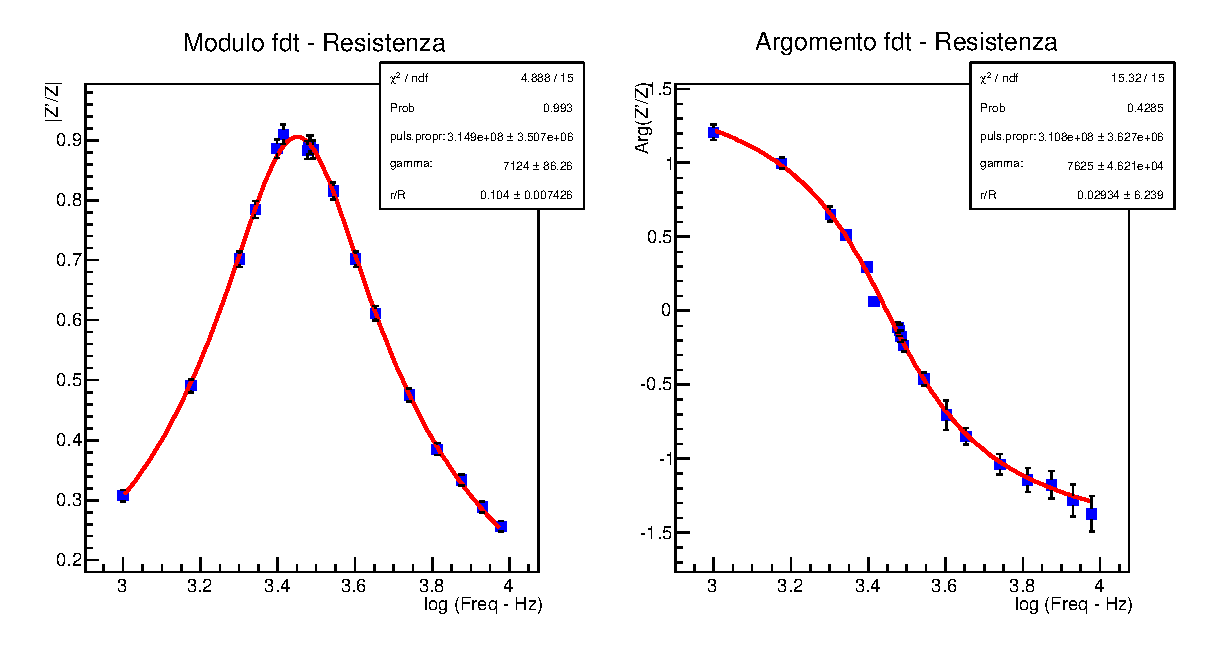
\includegraphics[scale=0.75]{Grafici/C4_P2_Res.eps}
\caption{
Circuito RLC serie.
AC.
Funzione di traferimento ai capi della resistenza.
}
\label{fig:C4_P2_Res}
\end{figure}







%%%%%%%%%%%%%%%%%%%%%%%%%%%%%%%%%%%%%%%%%%%%%%%%%%%%%%%%%%
%%%%%%%%%%%%%%%%%%%%%%% Capacità




\subsubsection{Capacità}

Funzione di trasferimento.
Si indica con $R$ la resistenza del resistore e con $r$ le altre resistenze (generatore, induttore).

\begin{align*}
f_{C}(w) = \frac{V_{C}}{V_{A}} 
= \frac{1}{ jwC ( (r+R) + j(wL - \frac{1}{wC}) ) }
= 
\frac{\frac{1}{w\frac{2\gamma}{w_0^2}}}
{( j(1+r/R) - \frac{1}{2\gamma}( w-\frac{w_0^2}{w} ) ) }.
\end{align*}

Modulo e fase.
Posto
$ y(w) = \frac{w - \frac{w_0^2}{w}}{2\gamma} $,
$ z(w) = \frac{1}{w\frac{2\gamma}{w_0^2}} $ e 
$ k = (1+r/R)$

\begin{align*}
& |\frac{V_{C}}{V_{A}}|  = z(w)( y(w)^2 + k^2)^{-\frac{1}{2}}
& Arg\frac{V_{C}}{V_{A}} = \arctan( \frac{k}{y(w)} )
\end{align*}


\begin{table}[H]
\begin{center}
\begin{tabular}{|r|r|r|r|r|}
\hline
\multicolumn{1}{|l|}{Freq} & \multicolumn{1}{l|}{Va} & \multicolumn{1}{l|}{Vb} & \multicolumn{1}{l|}{Fase } & \multicolumn{1}{l|}{Err Fase} \\ \hline
\multicolumn{1}{|l|}{Hz} & \multicolumn{1}{l|}{V} & \multicolumn{1}{l|}{V} & \multicolumn{1}{l|}{$\mu s$} & \multicolumn{1}{l|}{$\pm \mu s$} \\ \hline
\multicolumn{1}{|c|}{$\pm 1$} & \multicolumn{1}{c|}{$\pm 0.2$} & \multicolumn{1}{c|}{$\pm 0.08$} & \multicolumn{1}{l|}{} & \multicolumn{1}{l|}{} \\ \hline
20000 & 10.8 & 0.14 & 17.2 & 0.8 \\ \hline
10000 & 10.8 & 0.33 & 30.4 & 0.8 \\ \hline
8000 & 10.4 & 0.41 & 35.6 & 0.4 \\ \hline
6000 & 10.8 & 0.55 & 46 & 2 \\ \hline
4000 & 10.8 & 0.84 & 64 & 2 \\ \hline
2000 & 10.8 & 1.66 & 120 & 4 \\ \hline
1000 & 10.6 & 3.18 & 204 & 8 \\ \hline
500 & 10.4 & 5.48 & 330 & 20 \\ \hline
100 & 10.4 & 9.68 & 500 & 40 \\ \hline
50 & 10.4 & 10.00 & 440 & 40 \\ \hline
\end{tabular}
\end{center}
\caption{Ddp e Fase ai capi del condensatore.
Resistenza 11.000 (+50+50)  [$\Omega$].
Capacità  46    [$nF$].
Induttore 0.065 [$H$].}
\label{tab:C2_P2_cond}
\end{table}


\begin{figure}[H]
\centering
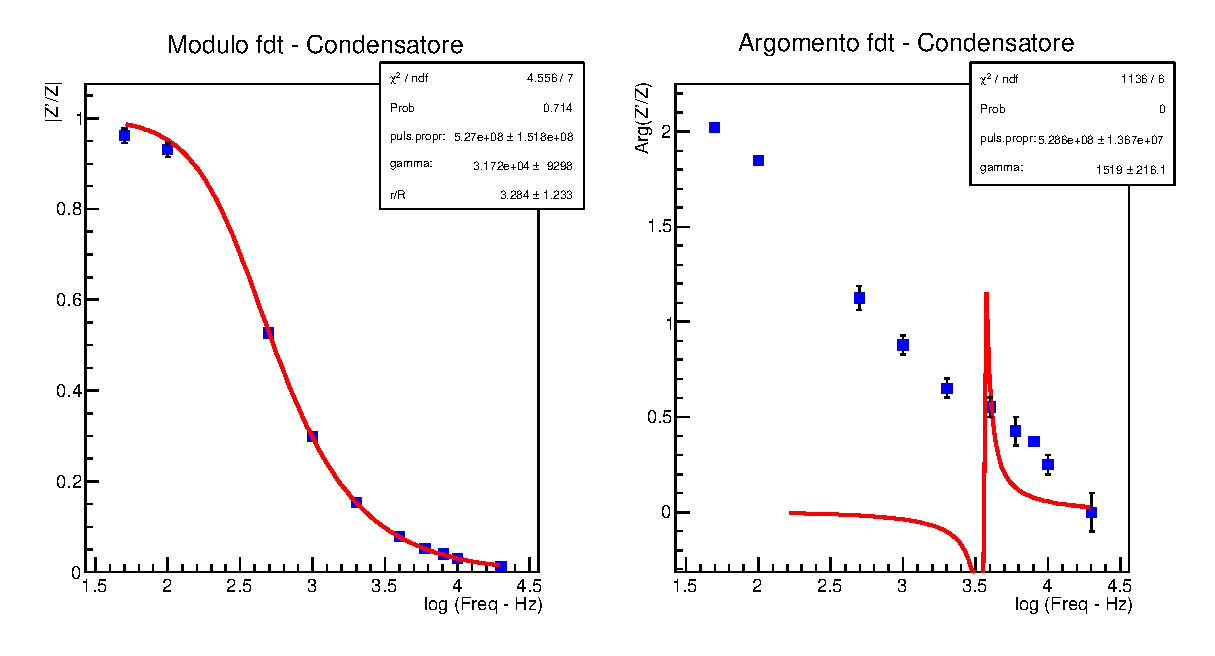
\includegraphics[scale=0.75]{Grafici/C4_P2_Cond.eps}
\caption{
Circuito RLC serie.
AC.
Funzione di traferimento ai capi della capacità.
}
\label{fig:C4_P2_Cond}
\end{figure}




%%%%%%%%%%%%%%%%%%%%%%%%%%%%%%%%%%%%%%%%%%%%%%%%%%%%%%%%%%
%%%%%%%%%%%%%%%%%%%%%%% Induttore




\subsubsection{Induttore}

Funzione di trasferimento.
Si indica con $R$ la resistenza del resistore e con $r$ le altre resistenze (generatore, induttore).

\begin{align*}
\frac{V_{L}}{V_{A}} 
= \frac{jwL}{ (r+R) + j(wL - \frac{1}{wC}) }
= 
\frac{\frac{w}{2\gamma}}
{ -j(1+r/R) + \frac{1}{2\gamma}( w-\frac{w_0^2}{w}) }.
\end{align*}

Modulo e fase.
Posto
$ y(w) = \frac{w - \frac{w_0^2}{w}}{2\gamma} $,
$ z(w) = \frac{w}{2\gamma} $ e 
$ k = (1+r/R)$

\begin{align*}
& |\frac{V_{C}}{V_{A}}|  = z(w)( y(w)^2 + k^2)^{-\frac{1}{2}}
& Arg\frac{V_{C}}{V_{A}} = \arctan( \frac{k}{y(w)} )
\end{align*}


\begin{table}[H]
\begin{center}
\begin{tabular}{|r|r|r|r|r|}
\hline
\multicolumn{1}{|l|}{Freq} & \multicolumn{1}{l|}{Va} & \multicolumn{1}{l|}{Vb} & \multicolumn{1}{l|}{Fase } & \multicolumn{1}{l|}{Err Fase} \\ \hline
\multicolumn{1}{|l|}{Hz} & \multicolumn{1}{l|}{V} & \multicolumn{1}{l|}{V} & \multicolumn{1}{l|}{$\mu s$} & \multicolumn{1}{l|}{$\pm \mu s$} \\ \hline
\multicolumn{1}{|c|}{$\pm 1$} & \multicolumn{1}{c|}{$\pm 0.2$} & \multicolumn{1}{c|}{$\pm 0.08$} & \multicolumn{1}{l|}{} & \multicolumn{1}{l|}{} \\ \hline
500 & 10.2 & 0.33 & 870 & 20 \\ \hline
1000 & 10.2 & 1.36 & 424 & 4 \\ \hline
2000 & 10.4 & 6.60 & 176 & 4 \\ \hline
20000 & 10.6 & 10.50 & 1 & 0.2 \\ \hline
30000 & 10.6 & 10.50 & 0.3 & 0.2 \\ \hline
\end{tabular}
\end{center}
\caption{Ddp e Fase ai capi dell'induttore.
Resistenza 1.000 (+50+50)  [$\Omega$].
Capacità  46    [$nF$].
Induttore 0.065 [$H$].
}
\label{tab:C2_P2_ind}
\end{table}

\begin{figure}[H]
\centering
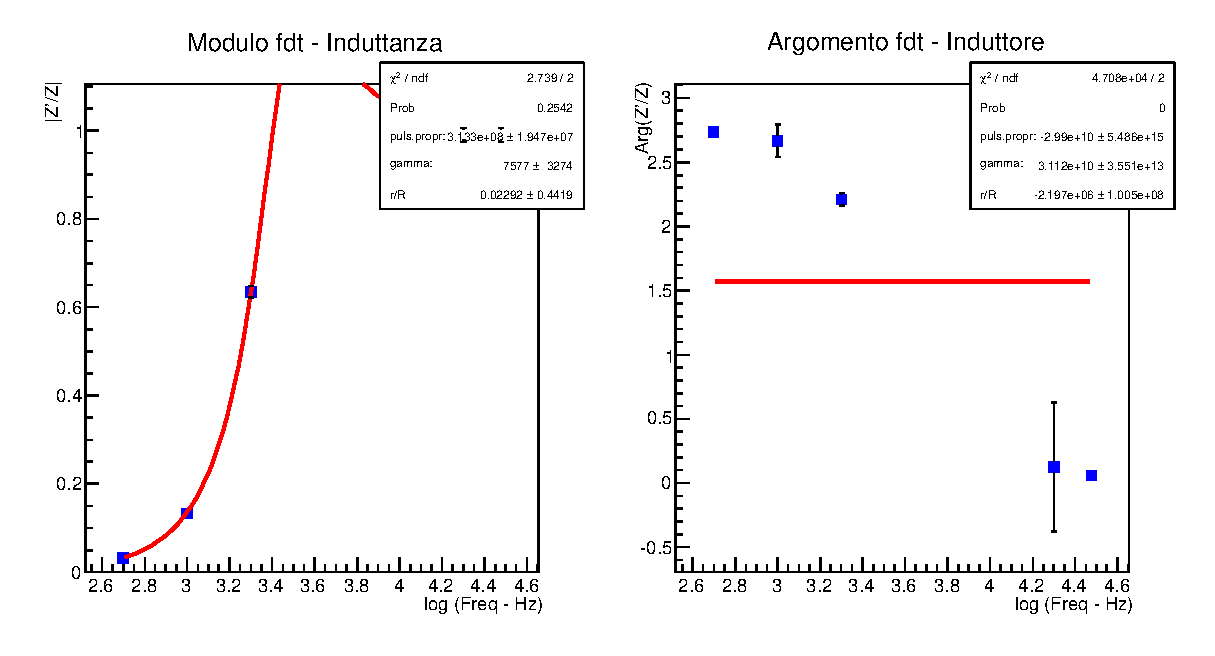
\includegraphics[scale=0.75]{Grafici/C4_P2_Ind.eps}
\caption{
Circuito RLC serie.
AC.
Funzione di traferimento ai capi dell'induttore.
}
\label{fig:C4_P2_Ind}
\end{figure}



\subsubsection{Conclusioni}

La tabella riporta le stime dei parametri del circuito.
Le tre colonne centrali riportano le stime della Parte 2 in corrente alternata. L'ultima colonna riporta le stime conclusive degli stessi parametri eseguite nella Parte 1 in corrente impulsata.

La parte 2 dell'esperimento riguardante le funzioni di trasferimento per capacità e induttore non è andata a buon fine. I risultati dei fit non vengono riportati perchè non affidabili.



\begin{table}[H]
\begin{center}
\begin{tabular}{|c|c|c|c|c|c|}

\hline
\multicolumn{ 1}{|c|}{Par.} & \multicolumn{ 1}{c|}{U.tà} & \multicolumn{ 3}{c|}{Funzioni di trasferimento RLC – AC} & \multicolumn{ 1}{c|}{RLC – DC} \\ \cline{3-5}

\multicolumn{ 1}{|c|}{} & \multicolumn{ 1}{c|}{} & Res & Cond & Ind & \multicolumn{ 1}{c|}{} \\ \hline

$r$ & $\Omega$ & $104\pm8\%$ &  &  & $100\pm1\%$ \\ 
$L$ & $H$ & $0.077\pm2\%$ &  &  & $0.066\pm2\%$ \\ 
$C$ & $nF$ & $41\pm4\%$ &  &  & $46\pm3\%$ \\ \hline
$R$ & $\Omega$ & \multicolumn{ 3}{c|}{$1000\pm1\%$} & $200\pm1\%$ \\ 
\hline

\end{tabular}
\end{center}
\caption{
Stime di $r$, $L$ e $C$.
$r$: resistenza parassita del circuito, comprensiva della resistenza del generatore e quella interna dell'induttore.
$L$: induttanza.
$C$: capacità.
$R$: resistenza del resistore non è stata oggetto di stima in quanto misurata direttamente, e riportata qui per completezza.
Nell'ultima colonna sono riportati i valori stimati nella Parte 1 in corrente continua.
}
\label{C4_P2_finale}
\end{table}

\break


\newpage

%%%%%%%%%%%%%%%%%%%%%%%%%%%%%%%%%%%%%%%%%%%%%%%%%%%%    
%%% O1

\section{Ottica 1 - Velocità della luce}

\subsection{Apparato}
%
    \begin{figure}[H]
    \centering
    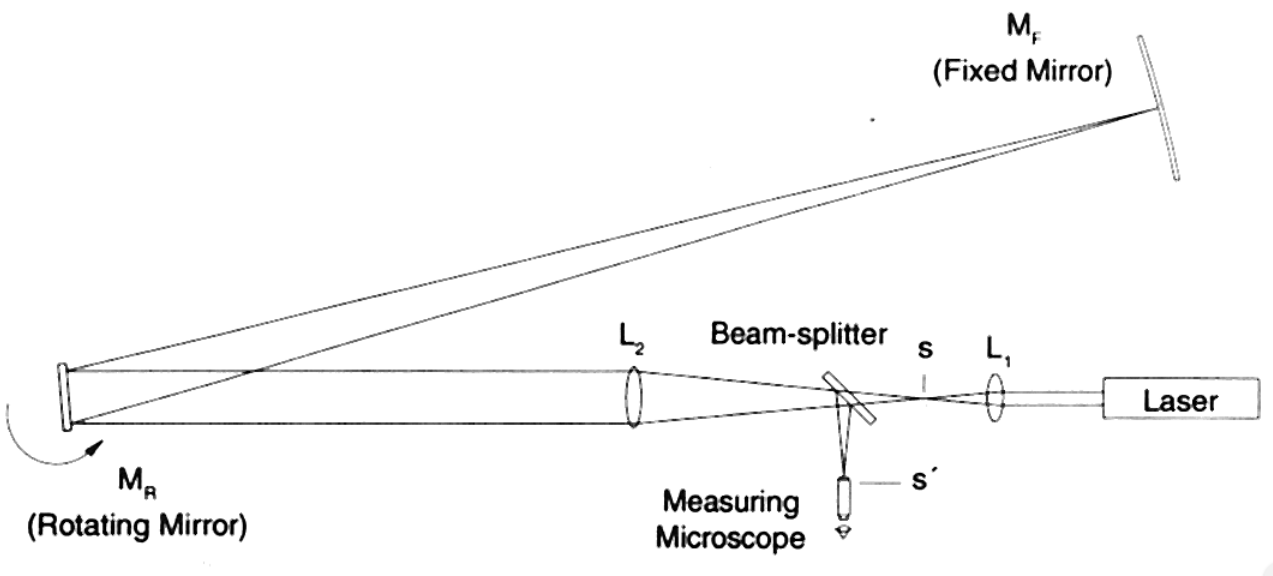
\includegraphics[scale=.3]{Grafici/O1_apparatus.png}
    \caption{Apparato sperimentale}
    \end{figure} 
%
I raggi paralleli all'asse ottico prodotti da una sorgente laser vengono focalizzati in un punto $s$ da una prima lente convergente $L1$.\\\\
%
Prima della seconda lente $L2$ uno specchio semiriflettente convoglia una parte del segnale ottico ad un microscopio, utilizzato per la lettura della misura.\\\\
%
La seconda lente $L2$, avente una distanza focale molto maggiore della prima lente $L1$ ma comunque inferiore alla distanza che la separa dal punto $s$, focalizza i raggi ad una distanza $ p>f2>f1 $.\\\\
%
\textcolor{red}{Prima del punto $A$ si trova interposto uno specchio imperniato su un supporto rotante che direziona i raggi verso uno specchio sferico di raggio $\sim A$; ciò fa sì che i raggi riflessi dallo specchio sferico ritornino sempre allo specchio rotante.}
COSA È IL PUNTO A?? VEDERE SCHEMA DI ALFREDO
\subsection{Misura della lunghezza focale della lente L2}
%
    \begin{figure}[H]
    \centering
    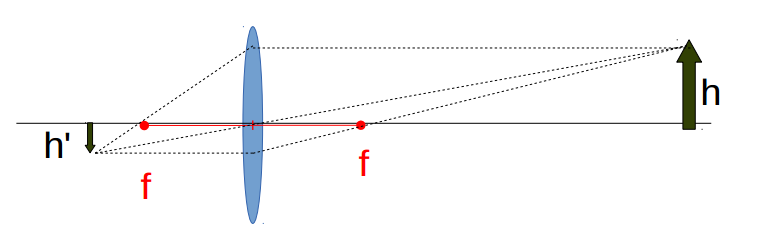
\includegraphics[scale=.4]{Grafici/O1_lente_focale.png}
    \caption{Lunghezza focale}
    \end{figure} 
%
%
Calibro illuminato da luce bianca molto intensa.\\\\
%
$p$ è la distanza calibro - lente L2;\\
$h$ è la dimensione effettiva dell'oggetto (apertura del calibro);\\
$h'$ è la dimensione dell'immagine dell'oggetto.\\
$q$ è la distanza immagine - lente L2, e si trova mediante la formula:
%
$$ \frac{h'}{h} = \frac{q}{p} $$
%
$f$ è la distanza focale della lente L2, che si ricava dalla legge dei punti coniugati:
$$ \frac{1}{p} + \frac{1}{q} = \frac{1}{f} $$
%
Ad una distanza $ p = 4610 \pm 10 $ mm, abbiamo variato l'apertura del calibro $h$ e abbiamo misurato $h'$ con il micrometro.
I dati sperimentali sono:\\
%
\begin{table}[H]
\centering
\begin{tabular}{|c|c|}
\hline
    $h$ 	&	$h'$		\\
    $mm$	&	$mm$		\\
    \hline
    10.00	&	0.60		\\
    15.00	&	0.88		\\
    18.60	&	1.07		\\
    20.00	&	1.14		\\
    25.00	&	1.43		\\
    30.00	&	1.69		\\
    35.00	&	2.00		\\
    40.00	&	2.31		\\
    45.00	&	2.59		\\
    50.00	&	2.83		\\
\hline    
\end{tabular}
\end{table}
%
Assumendo un errore di $0.02$ mm per $h'$, mediante propagazione errori e media pesata si ottiene:
$$ f = 249 \pm 1 \mathrm{ mm}$$
Valore nominale di 252 mm, ma incertezza sconosciuta.




\subsection{Velocità della luce}

Distanza L2 - specchio rotante:	$B = 0.315 \pm 0.001$ m;\\\\
%
%
Distanza specchio rotante - specchio fisso:	$D = 4.980 \pm 0.005$ m;\\
%
Distanza focale L2:	$f = 0.249 \pm 0.001$ m;\\
%
Distanza punto di convergenza del fascio laser (sorgente) - L2: $A = 0.261 \pm 0.001$ m, calcolato da
$$ A = \frac{(B+D)f}{B+D-f} $$
%
La velocità della luce si trova mediante la formula
$$ c = \frac{8 \pi A D^2 (\omega_{sx} + \omega_{dx})}{(D+B) \Delta S} $$
%
dove $\Delta S$ è lo spostamento letto sul micrometro del punto, osservato tra i due diversi versi di rotazione dello specchio.\\\\
%
La misura di $\Delta S$ è stata ripetuta 10 volte per ognuna delle due velocità di rotazione. Ecco di seguito riportati i dati:
\begin{table}[H]
    \centering
    \begin{tabular}{|c|c|c|c c|}
    \hline
    $x_L$ [mm]	&	$x_R$ [mm]	&	$\Delta S$ [mm]	\\
    ($\pm 0.01$)	&	 ($\pm 0.01$)	& ($\pm 0.02$)	\\
    \hline
        12.77	&	13.07	&	0.30	\\
        12.75	&	13.07	&	0.32	\\
        12.76	&	13.05	&	0.29	\\
        12.79	&	13.09	&	0.30	\\
        12.76	&	13.07	&	0.31	\\
        12.77	&	13.08	&	0.31	\\
        12.80	&	13.08	&	0.28	\\
        12.76	&	13.07	&	0.31	\\
        12.76	&	13.09	&	0.33	\\
        12.77	&	13.08	&	0.31	\\
    \hline
    \end{tabular}
    \caption{$\omega = 1550$}
    %\label{tab:my_label}
\end{table}
\begin{table}[H]
    \centering
    \begin{tabular}{|c|c|c|c c|}
    \hline
    $x_L$ [mm]	&	$x_R$ [mm]	&	$\Delta S$ [mm]	\\
    ($\pm 0.01$)	&	 ($\pm 0.01$)	& ($\pm 0.02$)	\\
    \hline
        12.49	&	12.68	&	0.19	\\
        12.53	&	12.68	&	0.15	\\
        12.55	&	12.69	&	0.14	\\
        12.49	&	12.68	&	0.19	\\
        12.50	&	12.69	&	0.19	\\
        12.50	&	12.68	&	0.18	\\
        12.49	&	12.67	&	0.18	\\
        12.50	&	12.68	&	0.18	\\
        12.49	&	12.68	&	0.19	\\
        12.83	&	12.98	&	0.15	\\
    \hline
    \end{tabular}
    \caption{$\omega = 750$}
    %\label{tab:my_label}
\end{table}
%
Valori ottenuti per la velocità della luce (errore per ogni misura calcolato con propagazione degli errori, poi effettuata la media pesata):
\begin{itemize}
    \item con $\omega_{dx} = \omega_{sx} = 1500 $, si trova $ c = 3.00 \cdot 10^8 \pm 0.01 \cdot 10^8 $, in perfetto accordo con il valore vero;
    \item con $\omega_{dx} = \omega_{sx} = 750 $, si trova $ c = 2.57 \cdot 10^8 \pm 0.09 \cdot 10^8 $, che si discosta del 14\% rispetto al valore vero. L'errore è probabilmente dovuto a un errore sistematico nella velocità di rotazione dello specchio. 
\end{itemize}
 



\newpage



%%%%%%%%%%%%%%%%%%%%%%%%%%%%%%%%%%%%%%%%%%%%%%%%%%%%    
%%% O2

\section{ Ottica 2 - Interferometro}
Laser utilizzato: Red Helium-Neon, $\lambda = 633$ nm.

\subsection{Interferometro di Fabry-Perot}

Si è misurato lo spostamento dello specchio mobile ($d$) nel conteggio di $\Delta k = 50 $ frange. Si è ricavata la lunghezza d'onda con:
$$\lambda = \frac{ 2 d \cos \theta }{\Delta k} $$
con l'approssimazione $\theta \approx 0$ (angolo tra l'asse ottico ed il riferimento sullo schermo per il conteggio delle frange).\\\\
%
Si sono ripetute le misure partendo da punti diversi della scala del micrometro, in modo da ottenere una curva di calibrazione del micrometro, ma non si sono osservati grossi discostamenti dal valore atteso di lughezza d'onda.\\\\
%
Tabella misurazioni:
%
\begin{table}[H]
    \centering
    \begin{tabular}{|c|c|c|}
    \hline
        $d_0$ iniz.	&	$d$	&	$\lambda$ \\
        $\mu m$	&	$\mu m$	&	$nm$ \\
        ($\pm 1$)   & ($\pm 1$) & ($\pm 42$)\\
    \hline
        800	&	17	&	680	\\
        700	&	16	&	640	\\
        600	&	17	&	680	\\
        400	&	16	&	640	\\
        300	&	16	&	640	\\
        200	&	16	&	640	\\
        100	&	16	&	640	\\
        6	&	16	&	640	\\
    \hline    
    \end{tabular}
\end{table}

%
L'errore di $\pm 42$ nm su $\lambda$ è calcolato mediante propagazione degli errori.\\
Il risultato finale ottenuto come media ed errore della media è:
$$\lambda = 650 \pm 16\; nm $$
Il valore vero di $\lambda$ si trova entro l'errore del risultato.
%


\subsection{Interferometro di Michelson}
$$ \lambda = \frac{2d}{\Delta k} $$
Ripetendo la misura 4 volte, con $\Delta k = 50$, è stata ottenuta sempre la stessa misura:
    $$ d = 284 \pm 1 \mu m $$
    $$ \lambda = 640 \pm 23 nm $$
Anche in questo caso, il valore teorico per la lunghezza d'onda è nell'intervallo di confidenza del risultato.
\subsection{Indice di rifrazione dell'aria}
L'indice di rifrazione dell'aria $n$ ha un andamento lineare con la pressione $P$, secondo la relazione $n = mP+1$.\\
%
È stato ricavato il coefficiente $m$ misurando $\Delta k$ per diversi valori di $(P_f-P_i)$, con la formula
%
    $$ m = \frac{\Delta k  \lambda_0}{2d(P_f-P_i)} $$
%
I dati sperimentali sono:
%
\begin{table}[H]
    \centering
    \begin{tabular}{|c|c|}
    \hline
        $\Delta P$	&	$\Delta k$	\\
        $kPa$	&	$-$	\\
        ($\pm2$)	&	($\pm 1$)	\\
        \hline
        78	&	17	\\
        84	&	18	\\
        84	&	17	\\
        48	&	10	\\
    \hline
    \end{tabular}
\end{table}
%
Il valore ottenuto (mediante media pesata) è $ m = 2.3 \pm 0.2 \cdot10^{-9}$ $\mathrm{Pa}^{-1}$.\\\\
%
Noto $m$ e usando $\lambda_0$ ricavata dall'esperimento di Michelson, si può calcolare $n_{aria}$ utilizzando come valore di $P$ il valore della pressione atmosferica ($101.5 \mathrm{kPa}$).
    $$ n_{aria} = 1+mP_{atm} =  1.00023 \pm 0.00002 $$ 
%
%
Il valore vero di $n$ a pressione atmosferica è $1.00029$, dunque a ritroso, il valore teorico di $m$ è $ 2.9 \cdot10^{-9}$ $\mathrm{Pa}^{-1}$. L'errore rispetto al valore teorico è del $21\%$.
\subsection{Indice di rifrazione del vetro}
%
$$ n = \frac{ (2d -\Delta k \lambda_0)(1-\cos\theta) }{ 2d (1-\cos\theta) - \Delta k \lambda_0}$$
%
I dati sperimentali sono:
%
\begin{table}[H]
    \centering
    \begin{tabular}{|c|c|}
    \hline
        $\theta$	&	$\Delta k$	\\
        gradi	&	$-$	\\
        \hline
        3.4	&	11	\\
        5.7	&	28	\\
        7.5	&	48	\\
        9.0	&	68	\\
        10.2	&	88	\\
        11.4	&	109	\\
    \hline
    \end{tabular}
\end{table}
%
Usando $\lambda = 633$ nm, ossia il valore vero, e calcolando l'errore come standard error della media, si trova:
$$ n_{vetro} = 1.56 \pm 0.02$$
I valori tipici di $n$ per il vetro sono compresi tra $1.5$ e $1.9$. Bisognerebbe in realtà avere più informazioni riguardo al tipo di vetro utilizzato nell'esperimento.




\subsection{Interferenza da righello}
Quando il fascio laser incide con un angolo molto vicino al piano del righello, si osserva interferenza. Questa è dovuta al fatto che le tacche dei millimetri si comportano da reticolo e i punti nello spazio tra le tacche come sorgenti coerenti. Sebbene la larghezza delle tacche sia molto maggiore della lunghezza d'onda, siccome il fascio è molto inclinato, la lunghezza d'onda "vista" dal reticolo è comparabile con la dimensione delle fenditure.\\\\
%
La figura di interferenza è descritta dalla seguente formula:
%
    $$ d(\cos\theta_i - \cos\theta_r) =  N \lambda $$
%
dove $d$ è il passo righello (1 mm), $\theta_i$ l'angolo di incidenza del laser, $\theta_r$ angolo di riflessione del massimo di ordine $N$.\\
Detti $y_0$ la posizione sullo schermo del massimo di ordine zero rispetto al piano del righello, $y_N$ la posizione del massimo di ordine $N$ e $L$ la distanza dello schermo dal punto di incidenza del laser sul righello, gli angoli di incidenza e riflessione si trovano così:
$$ \theta_i = \alpha = \mathrm{arctg}(y_0 / L) \quad ; \quad \theta_{r_N} = \mathrm{arctg}( y_N / L ) $$
%
Tabella risultati ($L = 115.5 \pm 1$ cm):
\begin{table}[H]
    \centering
    \begin{tabular}{|c|c|c|c c|}
    \hline
         ordine max	& $\theta_i$ & $\theta_r$ & $\lambda$ & errore $\lambda$\\
            -	&	°	&	°	&	nm	&	nm	\\
            -	& ($\pm 0.09$ ) & ($\pm 0.09$ ) & -	& -	\\
    \hline
            1	&	3.42	&	3.99	&	640	&	12	\\
            -1	&	3.42	&	2.78	&	606	&	10	\\
            2	&	3.42	&	4.55	&	689	&	14	\\
            -2	&	3.42	&	1.88	&	619	&	9	\\
    \hline
    \end{tabular}
    %\caption{Caption}
    %\label{tab:my_label}
\end{table}
si ottiene:
    $$ \lambda = 629 \pm 5 \; nm $$
In perfetto accordo con il valore nominale $633$ nm.




\newpage


%%%%%%%%%%%%%%%%%%%%%%%%%%%%%%%%%%%%%%%%%%%%%%%%%%%%    
%%% O3

\section{ Ottica 3 - Spettrometro}

\subsection{Spettri atomici }
Il  fenomeno  riguarda  l’interazione  tra  materia  allo  stato  gassoso  e  radiazione elettromagnetica. Quando un atomo viene investito da un fascio di fotoni accade che un elettrone, assorbendo un fotone, passi ad un livello energetico superiore, o stato eccitato. Questo stato è instabile e, dopo un tempo finito, l'elettrone tenderà a tornare allo stato di energia minima. La transizione da un livello energetico eccitato a uno stabile è accompagnata da emissione di radiazione. 
Si parla di assorbimento per la transizione di verso opposto.\\
%
Lo spettro di emissione o assorbimento di un materiale presenta in generale una moltitudine di informazioni circa la natura atomica, fisica e termodinamica dell'entità emittente. Alcuni tipici esempi sono temperatura, velocità, composizione chimica.
%
Per gas in condizioni di temperatura e pressione standard lo spettro spazia dalla radiazione infrarossa a quella ultravioletta in funzione della configurazione atomica.\\
%
Lo spettro di emissione nel visibile non è continuo. La presenza di righe spettrali di maggiore intensità nel caso degli spettri di emissione, o di righe scure in quelli di assorbimento, è indice del fatto che solo alcuni livelli energetici sono consentiti.
La distribuzione dei livelli energetici consentiti, attraverso la localizzazione delle lunghezze d'onda delle righe spettrali di un determinato elemento permette di caratterizzare la sua struttura atomica.
%
%
\subsection{Interferenza e diffrazione}
Quando un'onda attraversa un ostacolo opaco parte viene assorbita dalla superficie dell'ostacolo, producendo una deviazione dei raggi adiacenti. Tale fenomeno è detto diffrazione e può essere ben descritto tramite il principio di Huygens:\\
\textit{Nella propagazione di un'onda, ogni punto del fronte d'onda può essere considerato sorgente di onde secondarie, di modo che il fronte d'onda all'istante successivo risulti essere l'inviluppo delle onde secondarie che originano dal fronte d'onda precedente.}\\
Si hanno quindi due visioni perfettamente equivalenti per la descrizione dell'onda che propaga: come unico fronte d'onda in moto o come inviluppi successivi. Con questa descrizione, quando un'onda investe un ostacolo (come ad esempio una fenditura) i punti del fronte d'onda in diretto contatto con l'ostacolo vengono assorbiti mentre i rimanenti diventano sorgenti di onde secondarie. Il fronte d'onda oltre l'ostacolo diventa l'inviluppo dei fronti delle onde secondarie emesse dai punti non assorbiti dall'ostacolo.

Quando due onde si sovrappongono in una regione di spazio la perturbazione risultante è la somma delle due perturbazioni, secondo il Principio di Sovrapposizione. Nei punti in cui l'intensità risultante si annulla si parla di interferenza distruttiva, mentre nei punti in cui l'intensità risultante è massima si parla di interferenza distruttiva. 
Se si considerano onde piane sinusoidali di stessa lunghezza d'onda, del tipo:
    $$E_{1,2}(r,t) = E_{01,02}\cos(kr_{1,2}-\omega t +\phi_{1,2})$$
in un generico punto P, l'intensità dell'onda risultante sarà data da:
    $$ I = I_1 + I_2 + 2\sqrt{I_1I_2}\cos\delta $$
con $\delta = k(r_2-r_1) = k\Delta r$. Si vede che l'intensità è massima (interferenza costruttiva per $\cos\delta = 1$ e minima (interferenza distruttiva) per $\cos\delta = -1$, quindi:
    $$I_{max} \; \mathrm{per} \; k\Delta r = 2n\pi
    \quad\mathrm{e}\quad I_{min} \;\mathrm{per}\; k\Delta r = (2n+1)\pi $$
Se si considera un'onda composta da più lunghezze d'onda, poichè $ k = \lambda/2\pi $, si ha che lunghezze d'onda diverse hanno picchi di interferenza in punti diversi. Si ha così una scomposizione dello spettro dell'onda incidente e si possono ricavare le singole lughezze d'onda dalla condizione di interferenza per l'apparato sperimentale considerato.

\subsection{Rifrazione}
Quando un'onda elettromagnetica passa da un mezzo all'altro viene variata la velocità di propagazione a seconda delle proprietà elettromagnetiche ($\epsilon$ , $\mu$) del mezzo. Detto $n_k$ (indice di rifrazione) il rapporto tra la velocità della luce nel vuoto e nel mezzo k, le condizioni al contorno per il campo elettromagnetico sulla superficie di separazione tra i mezzi fanno si che l'onda subisca una deviazione tale da rispettare la legge di Snell:
    $$n_1\sin\theta_1 = n_2\sin\theta_2$$
Poichè l'indice di rifrazione del mezzo varia a seconda della lunghezza d'onda come:
    $$ n = A +  B/\lambda^2 $$
si ha che lunghezze d'onda differenti subiscono deviazioni differenti

\subsection{Fenomeno osservato e scopo dell'esperimento }
%
Il fenomeno osservato riguarda l'emissione di radiazione luminosa visibile generata da un gas rarefatto contenuto in un ampolla di vetro con due elettrodi connessi ad un'elevata differenza di potenziale.\\
%
L'emissione, una volta collimata e direzionata verso un dispositivo rifrangente, viene scomposta nelle lunghezze d'onda che la compongono.\\
%
L'oggetto della rilevazione sono perciò le righe spettrali e il relativo colore, la loro larghezza e distribuzione.\\
%
Su tale analisi influisce fortemente il mezzo rifrangente (analizzatore).\\
%
%
\paragraph{Scopo dell'esperimento }

\begin{itemize}
    
    \item misurazione delle righe spettrali di alcuni gas con l'obiettivo di identificare il materiale emittente.
    
    \item confronto di due mezzi rifrangenti, prisma e reticolo
    
\end{itemize}
%
%
%
\subsection{Descrizione dell'apparato }
%
\paragraph{Tubi di Plucker}{Un gas contenuto in un tubo lungo di vetro contente due elettrodi agli estremi viene sottoposto a una differenza di potenziale elevata. Gli elettroni del gas vengono quindi eccitati e, diseccitandosi, emettono luce.}
\paragraph{Spettroscopio}{Apparato costituito da una base con un nonio per la misura degli angoli, un telescopio che può essere allineato con la riga spettrale tramite un mirino posto sulla lente oculare.
La base era dotata di una rotella per affinare la misura, che purtroppo era rotta. Non è stato possibile sfruttare tutta la precisione del nonio in quanto, manualmente, l'errore variava al minuto d'arco, non al secondo.}
\paragraph{Prisma}{Prisma di vetro con un angolo al vertice (che è stato usato per la diffrazione della luce) di $62 \pm 1 °$}
\paragraph{Reticolo di diffrazione}{Essendo costituito da un film incollato su una lastra di vetro spessa, per evitare gli effetti di rifrazione
della luce nel vetro si è fatto in modo che la lastra di vetro fosse attraversata
dalla luce proveniente dal collimatore prima di essere diffratta dal reticolo. Nominalmente, la densità del reticolo è di 600 linee/mm che corrisponde a un passo d = 1667 nm}

\clearpage

\subsection{Reticolo: determinazione del passo del reticolo}
Un fascio collimato di luce di lunghezza d'onda nota viene fatto passare attraverso un reticolo per poterne determinare il passo tramite la condizione di interferenza:
    $$ d\sin\theta = n\lambda $$
Vengono quindi effettuate misure dell'angolo a cui compaiono le varie righe spettrali (massimi di interferenza).
%
Se il reticolo è posizionato perpendicolarmente al fascio collimato emesso e noto che la riga gialla della lampada al sodio ha lunghezza d'onda $ \lambda = 589 $ [nm], si stima il passo del reticolo con la seguente relazione

\begin{equation}
d = \frac{ 589 n }{ \sin\theta }
\end{equation}
% Fit
%
%    \begin{figure}[H]
%    \centering
%    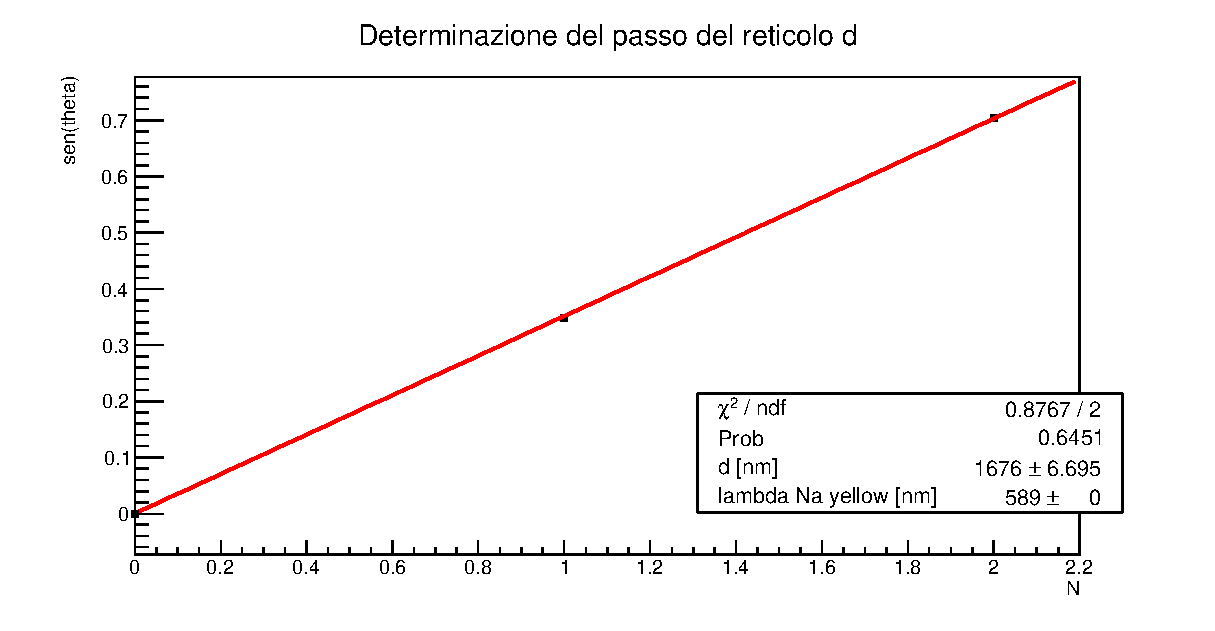
\includegraphics[scale=0.8]{Grafici/O3_P1_1_d.eps}
%    %\caption{}
%    \label{fig:C3_P2_RL}
%    \end{figure} 
%
%
%Fit usato: $ y = [1]/[0] x$\\
%dove $y = \sin(\theta)$ mediato (non corretto perchè non c'è bisogno, %sono simmetrici entro l'errore), $x = n$. Il parametro fissato è  $[1] = %\lambda_{yellow} = 589$ nm, e il parametro da stimare è $[0] = d$.\\\\
%
% Passo del reticolo stimato dal fit:
% $$d = 1676 \pm 7 \mathrm{ nm}$$
%
%
\begin{table}[H]
    \begin{center}
    \begin{tabular}{|l r|c|c|c|}
    \hline
            &   Ordine  &   $\theta$    & $\sin\theta$  &   d   \\
            &           &   rad         &   -           &   nm  \\
            &           &   $\pm0.01$   &   $\pm 0.004$ &   -   \\
        \hline
        sx  &   1       & 0.351         & 0.344         & 1713 \\ 
        dx  &   1       & 0.360         & 0.352         & 1671 \\ 
        \hline
        sx  &   2       & 0.748         & 0.680         & 1732 \\ 
        dx  &   2       & 0.797         & 0.715         & 1646 \\ 
        \hline
    \end{tabular}
    \end{center}
    \caption{ Posizioni angolari dei primi due massimi. Lampada al sodio. $\lambda = 589$ [nm] }
    \label{O3_P1_d}
\end{table}
%
%
Il valore di riferimento atteso è pari ad un passo di $1.667$ [nm] relativo a $600$ fenditure al [$\mu$m]. Questo dato possiede un errore intrinseco sul numero di linee. Non potendo stimare tale errore, assumiamo come valore teorico $1.67$ $\mu m$ consapevoli del fatto che possiede un errore.\\
Per calcolare l'errore di d è stata usata la formula di propagazione.
%
%
\begin{table}[H]
    \begin{center}
    \begin{tabular}{|l r|}
    \hline
        Valore stimato & $1.69 \pm 0.02$ $\mu m$ \\
        Valore di riferimento & $1.67$ $\mu m$ \\ 
    \hline
    \end{tabular}
    \end{center}
\end{table}
%
Considerati gli errori sperimentali, il valore trovato per $d$ è in buon accordo con quello teorico. Si esclude quindi l'eventuaità di asimmetria del sistema o di non perpendicolarità del fascio incidente
\clearpage
\subsection{Reticolo: determinazione della lunghezza d'onda per diverse lampade}
Noto dal punto precedente il passo del reticolo di diffrazione, si utilizza lo stesso procedimento di misura per indagare lo spettro di emissione di gas incogniti, facendo sempre attenzione alla perpendicolarità del raggio incidente. Sono state utilizzate le lampade etichettate B,C,D. Di seguito i risultati.\\
\subsubsection{Lampada B}
Dati:
\begin{table}[H]
\begin{center}
\caption{Dati lampada D}
\begin{tabular}{|c|cc|}
\hline
Colore	&	$\sin \theta$	&	err $\sin \theta$	\\
	&	rad	&	rad	\\ \hline
Verde	&	0.329	&	0.003	\\
Arancione	&	0.347	&	0.003	\\
Viola1	&	0.255	&	0.003	\\
Viola2	&	0.262	&	0.003	\\ \hline
\end{tabular}
\end{center}
\label{label}
\end{table}

Risultlati:
\begin{table}[H]
\begin{center}
\caption{Spettro Lampada B}
\begin{tabular}{|c|c|c|}
\hline
Colore & Lungh.Onda [nm] & Errore [nm] \\ 
\hline
MassimoViola & 420 & 8 \\
\hline
Viola1 & 410 & 8 \\ 
Viola2 & 420 & 8 \\ 
Azzurro1 & 450 & 7 \\ 
Azzurro2 & 470 & 7 \\ 
Verde1 & 540 & 7 \\ 
Verde2 & 550 & 7 \\ 
Arancione & 600 & 7 \\ 
\hline
\end{tabular}
\end{center}
\label{label}
\end{table}

%
\subsubsection{Lampada C}
Dati:
\begin{table}[H]
\begin{center}
\caption{Dati lampada C}
\begin{tabular}{|c|cc|}
\hline
Colore	&	$\sin \theta$	&	err $\sin \theta$	\\
	&	rad	&	rad	\\ \hline
Giallo	&	0.351	&	0.004	\\ \hline
\end{tabular}
\end{center}
\label{label}
\end{table}

Risultati:
\begin{table}[H]
    \begin{center}
    \caption{Spettro lampada C}
    \begin{tabular}{|c|c|c|}
        \hline
        Colore & Lungh.Onda [nm] & Errore [nm]\\ 
        \hline
        Giallo & 590 & 7 \\ 
        \hline
    \end{tabular}
    \end{center}
    \label{table:O3_P2-2_sodio}
\end{table}


%
\subsubsection{Lampada D}
Dati:
\begin{table}[H]
\begin{center}
\caption{Dati lampada D}
\begin{tabular}{|c|cc|}
\hline
Colore	&	$\sin \theta$	&	err $\sin \theta$	\\
	&	rad	&	rad	\\ \hline
Massimo Viola	&	0.250	&	0.005	\\
Viola1	&	0.244	&	0.005	\\
Viola2	&	0.252	&	0.005	\\
Azzurro1	&	0.266	&	0.004	\\
Azzurro2	&	0.278	&	0.004	\\
Verde1	&	0.325	&	0.004	\\
Verde2	&	0.329	&	0.004	\\
Arancione	&	0.357	&	0.004	\\ \hline
\end{tabular}
\end{center}
\label{label}
\end{table}

Risultati:
\begin{table}[H]
    \begin{center}
    \caption{Spettro Lampada D}
    \begin{tabular}{|c|c|c|}
        \hline
        Colore & Lungh.Onda [nm] & Errore [nm]\\ 
        \hline
        Verde & 550 & 5 \\ 
        Arancione & 580 & 5 \\ 
        Viola1 & 430 & 5 \\ 
        Viola2 & 440 & 5 \\ 
        \hline
    \end{tabular}
    \end{center}
    \label{label}
\end{table}

%
%
\subsubsection{Confronto con spettro del visibile}
\label{sec:reticolo_confronto} 
%
% Spettro lampade B, C e D
%
    \begin{figure}[H]
    \centering
    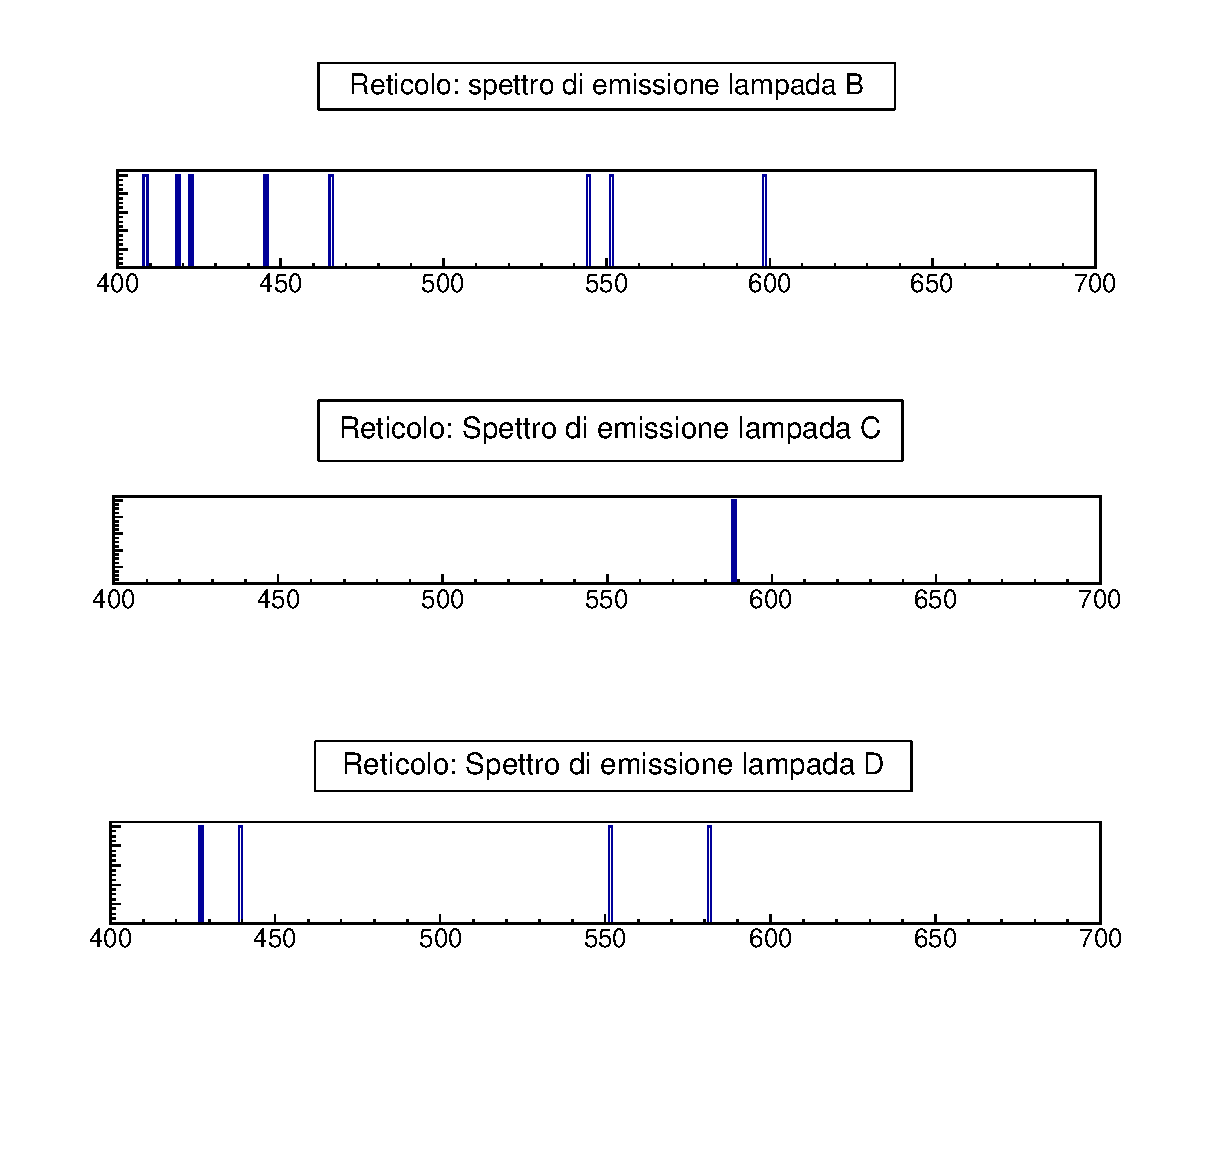
\includegraphics[scale=0.75]{Grafici/O3_P1_2_spectrum.eps}
%
    \includegraphics[scale=1.1]{Grafici/VISspectrum.jpg}
    %\caption{}
    \label{fig:C3_P2_RL}
    \end{figure} 
%
\clearpage
\subsection{Prisma: determinazione coefficienti A e B della formula di Cauchy}
\label{sec:prisma1}
Il fascio collimato di lunghezza d'onda nota viene rifratto attraverso un prisma. Sia $\alpha = 62 \pm 1 °$ l'angolo tra le facce attraverso cui avviene la diffrazione, misurato con un goniometro. Ruotando la base di un angolo $\delta$ l'angolo di rifrazione diminuisce fino a raggiungere un minimo. Il $\delta$ di minima deviazione (che dipende dalla lunghezza d'onda del raggio incidente) viene usato per calcolare l'indice di rifrazione del prisma ($n$), da:
    $$ n(\lambda) = \frac{\sin(\frac{\alpha + \delta(\lambda)}{2})}{\sin(\alpha/2) } $$
La misura di $\delta$ presenta una maggiore difficoltà di precisione in quanto il raggio deviato arresta il suo moto e lo inverte entro un intervallo di angoli non trascurabile (che è stato incluso nell'errore). Per minimizzare l'errore su questa misura, si è osservata l'inversione del moto su uno schermo posto un paio di metri di distanza. Ciò per massimizzare lo spostamento del fascio sullo schermo rispetto a piccole variazioni di angolo ($\Delta s = \theta r$) e rendere più precisa l'individuazione del punto di minimo.\\
%
Le lunghezze d'onda sono note: il gas utilizzato è il mercurio.\\
Gli indici di rifrazione così ottenuti vengono poi utilizzati per stimare i parametri A e B della legge di Cauchy, utilizzata poi negli esperimenti successivi.
    $$ n(\lambda) = A + B/\lambda^2 $$
Di seguito i dati sperimentali raccolti e i risultati ottenuti.\\
%
\begin{table}[H]
    \begin{center}
    \begin{tabular}{|c|c c|}
    \hline
        $\lambda$ [Hg]	&	$\delta$	&		err $\delta$ \\
        nm	&	rad	&		rad	\\
    \hline
        619.3	&	0.837	&		0.004	\\ 
        578.0	&	0.845	&		0.004	\\
        546.1	&	0.848	&		0.003	\\
        502.5	&	0.862	&		0.003	\\
        435.8	&	0.881	&		0.003	\\
        407.8	&	0.894	&		0.003	\\
        404.7	&	0.897	&		0.003	\\
    \hline
    \end{tabular}
    \end{center}
    %\caption{ }
    \label{O3_P2_1}
\end{table}


%
% coefficienti A, B
%
    \begin{figure}[H]
    \centering
    \includegraphics[scale=0.8]{Grafici/O3_P2_1_AB.eps}
    %\caption{}
    \label{fig:C3_P2_RL}
    \caption{Verifica legge di Cauchy. Fit: $y = [0] + [1]/x^{2}$ dove $y = n$, $x = \lambda$, e i parametri da stimare $[0] = A$ e $[1] = B$. }
    \end{figure} 
%
%
%
%
Coefficienti della formula di Cauchy stimati dal fit:
$$ A = 1.567 \pm 0.003 \quad ;\quad B = 9100 \pm 600 \;\mathrm{ nm^{2}} $$
%
\paragraph{Osservazioni:}{ Il $\chi^2$ risulta troppo basso. Si sospetta una sovrastima degli errori. Si applica il procedimento della stima dell'errore a posteriori come descritto nel paragrafo \ref{sec:C3_final}
%reference:Paragrafi/C3_finale.tex
Di seguito il risultato del nuovo fit.

    \begin{figure}[H]
    \centering
    \includegraphics[scale=0.8]{Grafici/O3_P2_1_AB_p.eps}
    %\caption{}
    \label{fig:C3_P2_RL}
    \caption{Verifica legge di Cauchy con errori stimati a posteriori. Fit: $y = [0] + [1]/x^{2}$  }
    \end{figure}
%
%
Da questo nuovo fit si ottiene:
$$ A = 1.567 \pm 0.001 \quad ; \quad B = 9100 \pm 200 \;\mathrm{ nm^{2}} $$
che vengono assunti come stima di A e B.    
}  

\clearpage
\subsection{Prisma: determinazione della lunghezza d'onda per diverse lampade}
\label{sec:prisma2}
Il fascio collimato di lunghezza d'onda incognita viene rifratto attraverso un prisma e viene misurato l'angolo di minima deviazione per calcolare le lunghezze d'onda dello spettro di emissione del gas. Valgono le stesse considerazioni sulle modalità di misura fatte nel paragrafo \ref{sec:prisma1}. Le lampade utilizzate sono la C e la D.\\
\\
Misurato $\delta$, si ottiene la lunghezza d'onda eguagliando le due espressioni dell'indice di rifrazione, con $\alpha$ noto ($62 \pm 1 °$) ed A e B ricavati da esperimento precedente. (Dove è stato sottinteso $\delta = \delta(\lambda)$ per alleggerire la notazione)
    $$ n(\lambda) = \frac{\sin(\frac{\alpha + \delta }{2})}{\sin(\alpha/2) } = A + B/\lambda^2 $$
quindi:
    $$ \frac{1}{\lambda^2} = \frac{\frac{ \sin( (\alpha + \delta)/2 ) }{\sin(\alpha/2) } - A}{B} $$
e:
    $$\lambda = \sqrt{ \frac{B}{ \frac{ \sin( (\alpha + \delta)/2 ) }{\sin(\alpha/2) } -A } } $$
\subsubsection{Lampada C}
Dati:
\begin{table}[H]
\begin{center}
\caption{Dati lampada C}
\begin{tabular}{|c|c|}
\hline
Colore	&	$\delta$	    \\
    	&	rad	            \\
    	&	$\pm 0.003 $	\\ \hline
Rosso1	&	0.830		    \\
Rosso2	&	0.830   	   	\\
Giallo	&	0.841   		\\
Verde1	&	0.847	    	\\
Verde2	&	0.853	    	\\
Verde3	&	0.860    		\\
Verde4	&	0.861		    \\
Blu1	&	0.867	    	\\
Blu2	&	0.876   		\\
Viola	&	0.879	    	\\ \hline
\end{tabular}
\end{center}
\label{label}
\end{table}

Risultati:
\begin{table}[H]
\begin{center}
\caption{Spettro Lampada C}
\begin{tabular}{|c|c|c|}
\hline
Colore & Lungh.Onda [nm] & Errore [nm]\\ 
\hline
Rosso & 680 & 60 \\ 
Giallo & 590 & 40 \\ 
Verde1 & 560 & 30 \\ 
Verde2 & 530 & 20 \\ 
Verde3 & 500 & 20 \\ 
Verde4 & 500 & 20 \\ 
Blu1 & 480 & 20 \\ 
Blu2 & 450 & 10 \\ 
Viola & 440 & 10 \\ 
\hline
\end{tabular}
\end{center}
\label{label}
\end{table}



\subsubsection{Lampada D}
Dati:
\begin{table}[H]
\begin{center}
\caption{Dati lampada D}
\begin{tabular}{|c|c|c|}
\hline
Colore  	&	$\delta$    	\\
	        &	rad		        \\
	        &	$\pm 0.003 $	\\ \hline
Rosso   	&	0.830		    \\
Arancione	&	0.840	    	\\
Giallo  	&	0.841   		\\
Verde1	    &	0.847		    \\
Verde2  	&	0.850	        \\
Blu	        &	0.876   		\\
Viola	    &	0.888	    	\\ \hline
\end{tabular}
\end{center}
\label{label}
\end{table}

Risultati:
\begin{table}[H]
\begin{center}
\caption{Spettro Lampada D}
\begin{tabular}{|c|c|c|}
\hline
Colore & Lungh.Onda [nm] & Errore [nm] \\ 
\hline
Rosso & 680 & 60 \\ 
Arancione & 600 & 40 \\ 
Giallo & 590 & 40 \\ 
Verde1 & 560 & 30 \\ 
Verde2 & 540 & 30 \\ 
Blu & 450 & 10 \\ 
Viola & 420 & 10 \\ 
\hline
\end{tabular}
\end{center}
\label{label}
\end{table}



\subsubsection{Confronto con spettro del visibile}
\label{sec:prisma_confronto}
%
% Spettro lampade C e D
%
    \begin{figure}[H]
    \centering
    \includegraphics[scale=0.8]{Grafici/O3_P2_2_spectrum.eps}
    %\caption{}
    \includegraphics[scale=1.2]{Grafici/VISspectrum.jpg}
    %\caption{}
    \label{fig:C3_P2_RL}
    \end{figure} 
%
\paragraph{Considerazioni:}{Utilizzando il prisma si possono osservare molte più righe spettrali che con il reticolo, ma di minore intensità. In alcune zone dello spettro (in particolare nel rosso) le linee risultano talmente fitte da sembrare un continuo, rendendo difficile l'individuazione dei singoli massimi. Si è attribuito perciò un errore maggiore a tali zone, stimato dall'ampiezza della banda di colore continuo osservata.}

\clearpage
\subsection{Conclusioni}
Come si può osservare nei paragrafi \ref{sec:reticolo_confronto} e \ref{sec:prisma_confronto} le lunghezze d'onda calcolate combaciano qualitativamente con il colore delle righe spettrali osservate in entrambi gli esperimenti (reticolo e prisma).

\paragraph{Confronto spettro con metodo del reticolo e del prisma}
%
{Il metodo di diffrazione attrverso il reticolo risulta produrre meno bande, ma di maggiore intensità e più facilmente analizzabili dallo sperimentatore. Mentre, come detto nelle Conclusioni della sezione \ref{sec:prisma2}, il metodo del prisma presenta una maggiore imprecisione nel determinare l'esatta posizione di un singolo massimo in quanto se ne osservano molti a distanza ravvicinata.\\
Si ipotizza quindi che il metodo del reticolo sia più efficace per determinare lo spettro con tipologie di esperimenti simili a questo, con analisi da oculare di un telescopio per determinare la posizione dei massimi. Invece con metodi di analisi meno soggetti all'errore umano (si pensa ad esempio all'esposizione di una lastra fotografica) potrebbe essere più efficace il metodo del prisma in quanto rivela una maggior quantità di righe spettrali.}
%
% Spettro lampada C
%
    \begin{figure}[H]
    \centering
    \includegraphics[scale=0.8]{Grafici/O3_C_lampadaC_spectrum.eps}
    %\caption{}
    \label{fig:C3_P2_RL}
    \end{figure} 
%
% Spettro lampada D
    \begin{figure}[H]
    \centering
    \includegraphics[scale=0.8]{Grafici/O3_C_lampadaD_spectrum.eps}
    %\caption{}
    \label{fig:C3_P2_RL}
    \end{figure} 
%
%
\paragraph{Identificazione materiali delle lampade}{
A causa dell'errore sperimentale troppo elevato, non si è riusciti a determinare con precisione gli elementi dal sito del NIST.}

\paragraph{Osservazioni aggiuntive}
\begin{itemize}
    \item Per poter utilizzare l’approssimazione di onda piana si deve realizzare una condizione di illuminazione corrispondente a una sorgente virtuale posta all’infinito. In tal modo è possibile considerare paralleli tutti i raggi uscenti dalla fenditura e porre la differenza di cammino ottico pari a $k d \sin\theta $
    \item Utilizzando questo spettrometro, si è previsto di riuscire a vedere circa 2 o 3 massimi a seconda della lunghezza d’onda.
    $$\sin\theta = n\frac{\lambda}{d} < 1 \Rightarrow n < \frac{d}{\lambda} \approx 3 $$
    Se ne osservano solamente 2, si ipotizza a causa delle condizioni di illuminazione della stanza.
    \item Il potere risolutivo del reticolo è $\frac{1}{nN}$, dove $N$ è il numero di fenditure. Non esssendo stata misurata la lunghezza del reticolo, non si è in grado di calcolarlo perchè, quindi non è noto $N$.
    \item Se fosse stato utilizzato un reticolo con passo più stretto, siccome $\sin\theta = n \frac{\lambda}{d}$, diminuendo $d$ aumenta l’angolo in cui viene osservata la lunghezza d’onda. Quindi si può diminuire l’errore relativo sull’angolo con misure di angoli grandi anche per i primi massimi.    
\end{itemize}



\newpage



%%%%%%%%%%%%%%%%%%%%%%%%%%%%%%%%%%%%%%%%%%%%%%%%%%%%    
%%% O4

\section{ Ottica 4 - Microonde}

\subsection{Ottica geometrica}
    \subsubsection{Legge di Cartesio}
        Inserire disegno schema esperimento\\
        Emettitore e ricevitore sono stati posizionati al centro di snodo delle guide. In modo che il segnale senza riflessione fosse a circa metà del misuratore, senza amplificazione (x1), lettura 0.32 $\pm$ 0.02 mA .
        %
        \begin{table}[H]
    \begin{center}
    \begin{tabular}{|c|c|}
        \hline
            $\theta_i$  & $\theta_r$    \\
            deg         & deg           \\
            $\pm$ 2     & $\pm 1$         \\ \hline
%    
            40 & 80  \\
            30 & 62  \\
            50 & 100 \\
            60 & 118 \\
            70 & 137 \\ \hline
%  
    \end{tabular}
    \end{center}
    \caption{ Angoli di incidenza, riflessione e intensità. Distanza ER dal centro 20 cm.}
    \label{O4_P1_cartesio}
\end{table}

        \paragraph{Note}{ L'emettitore emette onde anche fuori dall'altezza dello specchio (perchè è troppo basso) quindi si perde intensità anche per quello.\\
        Emettitore è lasco sul binario, quindi abbiamo aumentato l'errore.}
%
%
%
    \subsubsection{Rifrazione}
%
        \paragraph{ Indice di rifrazione del polistirolo}
        Il prisma di polistirolo, posto lungo l'asse ottico non ha provocato variazioni sensibili dell'intensità del segnale. La verifica è stata ottenuta togliendo e inserendo il prisma a diversi angoli di inclinazione del ricevitore, verificando l'assenza di variazioni significative del segnale ricevuto. Si pone perciò
%
            \[  n_{pol} = n_{aria}.  \]
%
        \paragraph{ Indice di rifrazione dello styrene }
        La misura dell'angolo del prisma $ \alpha = 23 \pm 1 $ gradi, è stata ottenuta con l'utilizzo del goniometro e del profilo sagomato del prisma su un foglio di carta.\\
%
        Il prisma è stato posizionato con la faccia verso il raggio incidente ortogonale all'asse ottico, in modo da creare una sola rifrazione.\\
%
        L'angolo $ \theta_{r} $ è l'angolo di rifrazione del raggio uscente dal prisma, misurato con il goniometro imperniato sulle guide metalliche.\\
            $$ \alpha = 23 \pm 1 \mathrm{°}$$ 
            $$ \theta_r =  33 \pm 1 ° $$
%        
        Posto $ n_{aria} = 1 $, il rapporto fra i seni fornisce l'indice di rifrazione del materiale
    
            $$ n = \frac{\sin( \alpha )}{ \sin( \theta_{r} ) } = 1.39 \pm 0.04. $$ 

\subsection{Polarizzazione}
    \subsubsection{Legge di Malus}
        Posti emettitore e ricevitore lungo la stessa retta e inclinando attorno a tale asse l'emettitore di un angolo $\gamma$, intenità letta dal ricevitore varia, secondo la legge di Malus, come:
            $$ I = I_0 \cos^2\gamma $$
        Di seguito i dati sperimentali raccolti.
    \begin{table}[H]
    \begin{center}
    \begin{tabular}{|c|c|c|}
\hline
        $ \gamma $	&	Intensità	&	Errore I	\\
        rad	&	mA	&	mA	\\
        $ \pm 0.02 $	&	-	&	-	\\ 
        \hline
        0.00	&	7.8	    &	0.2	    \\
        0.26	&	7.2	    &	0.2	    \\
        0.52	&	8.0	    &	0.2	    \\
        0.79	&	3.4	    &	0.2	    \\
        0.87	&	2.0	    &	0.2	    \\
        0.96	&	1.20	&	0.06	\\
        1.05	&	0.51	&	0.06	\\ 
        \hline
    \end{tabular}
    \end{center}
  % \caption{}
  %  \label{O4_P2_malus}
\end{table}
%
%
%%%%%%%%%%%%%%%%%%%%%%%%%%%%%%%%%%%%%%%%%%%%%%%%%%%%%%%%%%%%
%%%%%%%%%%%%%%%%%%%%%%%%%%%%%% FIT %%%%%%%%%%%%%%%%%%%%%%%%%
%%%%%%%%%%%%%%%%%%%%%%%%%%%%%%%%%%%%%%%%%%%%%%%%%%%%%%%%%%%%
%
%
    \begin{figure}[H]
        \centering
        \includegraphics[scale=0.8]{Grafici/O4_P2_malus.eps}
        \caption{Fit: $ I = I_0 \cos^2\gamma $ }
        \label{fig:C3_P2_RL}
    \end{figure} 
    %\subsubsection{Filtro polarizzatore}
    %non ci è uscito
    
    \subsubsection{Angolo di Brewster}
        Non è stato possibile prendere angoli superiori a 65° per limitazioni dovute alla strumentazione. Si osserva che l'intensità della corrente tende a zero all'aumentare dell'angolo, ma non si è in grado di determinare l'angolo esatto.\\
        Supponiamo che oltre all'effetto polarizzante della riflessione sul polietilene, si verifichi anche un effetto di interferenza tra l'onda riflessa dalla superficie e l'onda che giunge diretamente da dall'emettitore, \textcolor{red}{sopratutto ad angoli grandi?}
        \begin{figure}[H]
            \centering
            \includegraphics[scale=0.8]{Grafici/O4_P2_brewster.eps}
            \caption{Determinazione dell'angolo di Brewster}
            \label{fig:O4_P2_brewster}
        \end{figure}

\subsection{Misura di lambda}
%
Detta $\Delta l$ la differenza tra i due cammini ottici del sistema in considerazione, si ottiene che per i punti di interferenza costruttiva 
    $ \Delta l = n \lambda $, 
mentre per i punti di interferenza distruttiva
    $ \Delta l = (n + 1/2) \lambda $.\\
Notazioni utilizzate:\\
    $x_e$: posizione dell'emettitore su asse x\\
    $x_r$: posizione del ricevitore su asse x\\
%
\subsubsection{Onde stazionarie}
    Riduciamo l'errore sulla misura guardando lancetta con fattore amplificazione 10x fino all'intorno del max. Una volta al max cambiamo su 30x, per poter individuare il massimo più finemente.\\
   % \textbf{Oss}: qui max e min, quindi metà dell'eperimento di fabry perot (massimi consecutivi)\\
    \textbf{Oss}: questo metodo molto più efficiente di Fabry-Perot. La lancetta non oscilla così tanto e il sistema non è così sensibie alle perturbazioni esterne \\
    Emettitore fisso a $ x = 30.0 \pm 0.1 cm $ dallo zero di riferimento.
    Di seguito riportate le posizioni del ricevitore e tipo di picco corrispondente\\
%
    \begin{table}[H]	
\begin{center}
\begin{tabular}{|c|c|}
\hline
    $x_r$	&	Max/min	\\
    cm	&	-	\\
    $\pm 0.1 $	&	-	\\ \hline
    89.3	&	Max	\\
    90.0	&	Min	\\
    90.7	&	Max	\\
    92.2	&	Max	\\
    92.9	&	Min	\\
    93.7	&	Max	\\ \hline    
\end{tabular}
\end{center}
\end{table}
%
    Detta $d$ distanza tra due massimi successivi o due minimi successivi.
    $$ \lambda = 2d = 2.9 \pm 0.2 cm $$
    errore stimato con propagazione.\\
%
\subsubsection{Interferenza da doppia fenditura}
    Distanza tra le fenditure: $7.5 \pm 0.1 cm$\\
    Otteniamo:
        $$ \lambda = d\sin\theta/n = 2.5 \pm 0.1 cm$$
    errore stimato con propagazione.\\
    %
    Misure effettuate:
    \begin{table}[H]
\begin{center}
\begin{tabular}{|c|c|}
\hline
    Angolo	&	Ordine max	\\
    °	&	n	\\
    $\pm 2$	&	-	\\ \hline
    20	&	1	\\
    44	&	2	\\
    57	&	3	\\
    22	&	1	\\
    47	&	2	\\
    58	&	3	\\ \hline
\end{tabular}
\end{center}
\end{table}
%
\subsubsection{Specchio di Lloyd}
    \textbf{Notazioni e formule}\\
    %inserire immagine
    asse x: tra emettitore/ricevitore\\
    asse y: lungo direzione movimento specchio\\
    Cammino1 quello seguito dall'onda diretta\\ Cammino2 quello seguito dall'onda riflessa\\
    Consideriamo come origine (0,0) il centro del goniometro\\
%
    $y_s$: posizione dello specchio su asse y\\
    Cammino2 = 
        $\sqrt{ x^2_e + y^2_s } + \sqrt{ x^2_r + y^2_s }$\\
%
    Troviamo come risultato:\\
    $$\lambda = 2.7 \pm 0.1 cm$$
    errore stimato come standard error.\\
%
    \begin{table}[H]
\begin{center}
\begin{tabular}{|c|c|c|}
%	
    \multicolumn{3}{c}{Misura 1 con: $ x_e = 37.5 \pm 0.1 cm $ , $ x_r = 32.5 \pm 0.1 cm$}\\ \hline
    $y_s$	&	Ordine	&	$\lambda$	\\
    cm	&	n	&	cm	\\
    $\pm$ 0.1	&	-	&	$\pm$0.1	\\\hline
    15.4	&	2° minimo	&	2.6	\\
    18.8	&	3° minimo	&	2.7	\\
    13.3	&	2° massimo	&	2.5	\\
    17.0	&	3° massimo	&	2.6	\\ \hline
%
    \multicolumn{3}{c}{Misura 2 con: $ x_e = 27.5 \pm 0.1 cm $ , $ x_r = 27.5 \pm0.1 cm$} \\ \hline
%
    $y_s$	&	Ordine	&	$\lambda$	\\
    cm	&	n	&	cm	\\
    $\pm$0.1	&	-	&	$\pm$0.1	\\ \hline
    14.5	&	2° minimo	&	2.9	\\
    17.0	&	3° minimo	&	2.8	\\
    12.5	&	2° massimo	&	2.7	\\
    16.0	&	3° massimo	&	2.9	\\ \hline
\end{tabular}
\end{center}
\end{table}
%
\subsubsection{Parte 4: Interferometro di Fabry Perot}
    Fonti di errore: i supporti degli specchi erano molto sensibili alle più piccole oscillazioni, producento alterazioni dei risultati apprezzabili. Siamo stati attenti a non toccare il tavolo.\\
    Detta $d$ la distanza tra due massimi successivi, si ha che:
        $$ \lambda = 2d = 2.7 \pm 0.2 cm$$
    errore stimato con propagazione.\\
%
    Misure effettuate:\\
    \begin{table}[H]
\begin{center}
\begin{tabular}{|c|c|c|}
\hline
    x specchio2	&	$\lambda$	\\
    cm	&	cm	\\
    $\pm 0.1 $	&	$\pm 0.4$	\\ \hline
    55.2	&	-	\\
    54.0	&	2.4	\\
    52.5	&	3.0	\\
    51.1	&	2.8	\\
    49.8	&	2.6	\\
    48.7	&	2.2	\\
    47.1	&	3.2	\\
    45.7	&	2.8	\\ \hline
\end{tabular}
\end{center}
\end{table}
%
\subsubsection{Interferometro di Michelson}
    Le misure sono state fatte prima muovendo lo specchio L1 lugo l'asse x e poi L2 lungo l'asse y.\\
    \begin{table}[H]
\begin{center}
\begin{tabular}{|c|c|}
\hline
    $ x_{L1} $	&	$\lambda$	\\
    cm	&	cm	\\
    $ \pm 0.1 $	&	$ \pm 0.4 $	\\ \hline
    155.2	&	-	\\
    153.8	&	2.8	\\
    152.3	&	3.0	\\
    150.8	&	3.0	\\
    149.5	&	2.6	\\ \hline
    $ y_{L2}$	&	Lambda	\\
    cm	&	cm	\\
    $ \pm 0.1 $	&	$ \pm 0.4 $	\\ \hline
    84.7	&	-	\\
    86.1	&	2.8	\\
    87.6	&	3.0	\\
    89.1	&	3.0	\\
    90.5	&	2.8	\\ \hline
\end{tabular}
\end{center}
\end{table}
    Risultato:
        $$\lambda = 2\Delta x = 2\Delta y = 2.9 \pm 0.2 cm$$
    errore stimato con propagazione.\\
%
\subsubsection{Diffrazione di Bragg}

Il piano reticolare scelto è la diagonale del cubo.
Per ogni misura, è stato fatto ruotare il cubo di 1 grado e il braccio del ricevitore di 2 gradi (entrambi in senso orario), ed è stata letta l'intensità di corrente rilevata. Di seguito il grafico dei dati sperimentali:

    
    \begin{figure}[H]
    \centering
    \includegraphics[scale=0.8]{Grafici/O4_P3_Bragg.eps}
    %\caption{}
    \label{fig:O4_P3_Bragg}
    \end{figure} 
%
La distanza tra piani di diffrazione misurata è $d = 2.7$ cm. Il primo massimo ($n = 1$) si trova a $ \theta = 31$ gradi. L'errore sul grado è stato stimato $0.5$ gradi.\\
%
Dalla formula $$2 d \sin(\theta) = n \lambda $$
si ottiene 
$$ \lambda = 2d = 2.8 \pm 0.1 cm $$
In accordo con il valore nominale.
%

\subsection{Riassunto risultati}
    \begin{table}[H]
    \centering
    \begin{tabular}{|l|c c|}
        \hline 
           Esperimento & $\lambda$ [cm] & err [cm]   \\ \hline
        1: Onde Stazionarie & 2.9   & 0.2   \\
        2: Doppia Fenditura & 2.5   & 0.1   \\
        3: Lloyd            & 2.7   & 0.1  \\
        4: Fabry-Perot     & 2.7   & 0.2   \\ 
        5: Michelson        & 2.9   & 0.1   \\
        6: Bragg            & 2.8 & 0.1   \\ \hline
    \end{tabular}
\end{table}
%

\newpage


\end{document}